% Plantilla realizada por Alberto Brunete (UPM).

%parametros de tipo libro
\documentclass[10pt,a4paper]{book}

%idioma español y acentos
\usepackage[spanish, es-tabla]{babel}
%\usepackage[latin1]{inputenc}
\usepackage[utf8]{inputenc}
\usepackage{float}
%algunos sÌmbolos matem·ticos y paquete para usar subim·genes
\usepackage{amsmath}
\usepackage{amsfonts}
\usepackage{amssymb}
\usepackage{graphicx}
\usepackage{pgfplots}
\usepackage{caption}
\usepackage{subcaption}
%M·rgenes
\usepackage[left=3cm,top=3cm,right=3cm,bottom=3cm]{geometry}

%
\usepackage{multicol}

%para generar índice con hipervínculos
\usepackage{hyperref}

%parametros del documento (sus propiedades)
\hypersetup{
    pdftitle={Martin Augusto Reigadas Teran - TFG - 2022},
    pdfsubject={TFG - 2022},
    pdfauthor={Martin Augusto Reigadas Teran},
    pdfkeywords={palabraclave1} {palabraclave2} {palabraclave3},
    colorlinks,
    citecolor=black,
    filecolor=black,
    linkcolor=black,
    urlcolor=black,
}

\usepackage{cite}
\usepackage{epstopdf}
\usepackage{array}
\usepackage{multirow}
\sloppy
\epstopdfsetup{outdir=./pdf}

%\graphicspath{ {./graficasCasos_images/} }
%empieza el documento
\begin{document}  

%elementos antes del trabajo en sÌ se meten dentro de frontmatter
\frontmatter

%cada incluye referencia a un archivo de tipo .tex
\begin{titlepage}
\begin{center}
%forma de introducir imágenes. el \\[0.5 cm] de final de línea introduce un salto de ese tamaño.
%width=1\textwidth indica el tamaño de la imágen (valores entre 0-1). 

\includegraphics[width=1\textwidth]{figuras/cabecera.png}  \\[0.5 cm]

\LARGE UNIVERSIDAD POLITÉCNICA DE MADRID \\ [1 cm]

\LARGE ESCUELA TÉCNICA SUPERIOR DE INGENIERÍA Y DISEÑO INDUSTRIAL \\ [1 cm]

\LARGE Grado en Ingeniería Electrónica y Automática Industrial\\ [1 cm]

\LARGE \textbf{TRABAJO FIN DE GRADO}\\[0.75 cm]

\Huge \textsc{Modelado y simulación de espaciadores nanométricos para su aplicación en dispositivos TPVs de campo cercano}\\[1 cm]

\LARGE Martin Augusto Reigadas Teran \\[0.5 cm]
%flushleft alinea a la izquierda el texto
\begin{flushleft}
\Large
\emph{Tutor:} {Pablo García-Linares Fontes}\\
Departamento de Ingeniería Eléctrica, Electrónica, Automática y Física Aplicada\\
\emph{Cotutora:} Esther López Estrada\\
Instituto de Energía Solar\\
\end{flushleft}

%rellena de blanco el resto de la página para escribir abajo del todo
\vfill

% Bottom of the page
{\large Madrid, Septiembre, 2022}
%SE ponen al final firmas.tex
%\end{center}
%\end{titlepage}
\cleardoublepage 
\end{center}
\end{titlepage}


%Licencia opcional

\cleardoublepage

\begin{flushleft} \large
\textbf{TÌtulo:} Modelado de espaciadores nanométricos para un convertidor termo-fotovoltaico \\
\textbf{Autor:} Martin Augusto Reigadas Teran\\
\textbf{Tutor:} Pablo García-Linares Fontes \\ 
\textbf{Cotutor:} Esther López Estrada y Alejandro Datas\\ [1 cm]

\end{flushleft} 

\begin{center} \LARGE
EL TRIBUNAL \\ [1 cm]
\end{center}

\begin{flushleft} \LARGE
Presidente: \\ [1 cm]
Vocal: \\ [1 cm]
Secretario: \\ [1.5 cm]
\end{flushleft}

\large
Realizado el acto de defensa y lectura del Trabajo Fin de Grado el día ... de ....................   de ... en .........., en la Escuela Técnica Superior de Ingeniería y Diseño Industrial de la Universidad Politécnica de Madrid, acuerda otorgarle la CALIFICACIÓN de: \\ [2 cm]

\begin{center}
 \large VOCAL \\ [2.2 cm]
\end{center}

\begin{minipage}{0.5\textwidth}
 \begin{flushleft}
 \large SECRETARIO
\end{flushleft}
\end{minipage}
\begin{minipage}{0.5\textwidth}
\begin{flushright}
 \large PRESIDENTE
\end{flushright} 
\end{minipage}

\chapter{Agradecimientos}

Agradezco a mi tutor Pablo por darme la oportunidad de realizar un trabajo dentro de las líneas de investigación de la termo-fotovoltaica y contribuir a esta misma, permitirme explorar por mi cuenta y experimentar como la investigación llega a ser.\\\\
A mi cotutora Esther por brindarme tanto apoyo durante la realización del trabajo, explicándome conceptos en mayor detalle y permitirme ir más allá con el trabajo. También agradezco a Alejandro Datas por brindarme apoyo para no salirme de los objetivos de este trabajo.\\\\
Gracias a los tres por permitirme participar en la elaboración del póster presentado en la treceava conferencia mundial en la generación de electricidad termo-fotovoltaica (\href{https://www.tpv-13.org/}{TPV-13}) de Abril del 2022, compartida con la dieciochoava conferencia internacional de sistemas fotovoltaicos de concentración (\href{https://www.cpv-18.org/}{CPV-18}).\\\\  
A mi padre por siempre apoyarme durante la carrera, y a mi hermana Andrea por brindarme apoyo cuando más lo necesitaba y por siempre estar ahí encargándote de muchas cosas.\\\\
A mis amigos, Andrea, ZhanYao y Tesa con los cuales he pasado estos duros cuatro años juntos estudiando, trasnochando realizando los trabajos de las asignaturas, viviendo nuevas experiencias y aprendiendo bastante cosas más allá de la ingeniería.\\\\
A Yvonne por empujarme a salir de mi zona de confort, hacer lo que hay que hacer cuando se debía y aprender a como seguir con la vida.\\\\
A Noelia por estar ahí gran parte del tiempo de realización de este trabajo, apoyándome en cada fase y recordándome de tomar descansos.\\\\
A la Asociación del Cubo por permitirme conocer a gente tan bonita como Rafael, que siempre ha brindado su apoyo y llegando a ser de gran ayuda para la realización de este trabajo. Al CREA por permitirme conocer a más gente que le encanta la electrónica y pasar unas buenos ratos con los proyectos.\\\\

%chapter introduce un nuevo capítulo
\chapter{Resumen}

Este proyecto se resume en.................

\paragraph{Palabras clave:} palabraclave1, palabraclave2, palabraclave3.

\chapter{Abstract}

In this project...

\paragraph{Keywords:} keyword1, keyword2, keyword3.

%genera índice
\tableofcontents
\addcontentsline{toc}{chapter}{Índice}

%Índice de figuras.
\listoffigures

%Índice de tablas.
\listoftables

%Empieza la parte descriptiva del trabajo
\mainmatter

\chapter{Introducción}

En este capítulo no deben faltar los siguientes apartados:

\section{Motivación del proyecto}

En los últimos años el consumo de energía primaria en España ha aumentado significativamente de unos 88455 ktep($\sim1.03E12 \ kWh$) en 1990 a unos 126107 ktep($\sim 1.43E12 \ kWh$) en 2019, que equivale a un aumento del 42\% respecto a su valor en 1990, llegando a ser su valor máximo unos 146891 ktep($\sim 1.71E12 \ kWh$) en 2007.\\\\
De 2008 a 2014, como consecuencia de la crisis económica el consumo energético disminuyó hasta unos 117824 ktep ($\sim 1.37E12 \ kWh$) en 2014, recuperándose a partir del 2015, como se puede observar en la figura \ref{fig:demandaenergiaprimariaproporcion1990}. \\


\begin{figure}[H]
	\centering
	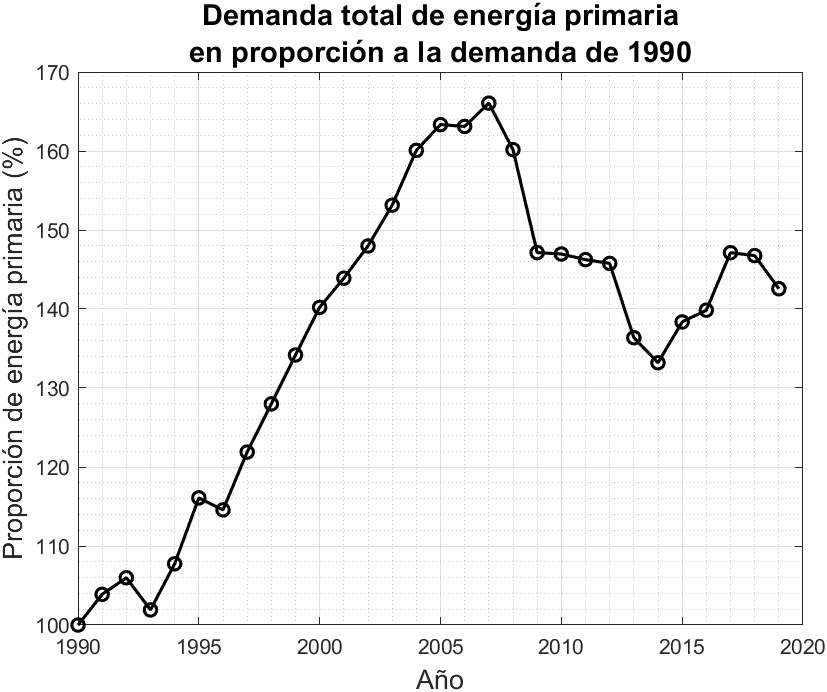
\includegraphics[width=10cm, height=7cm]{figuras/DemandaEnergiaPrimariaProporcion1990}
	\caption[Relación entre demanda total de energía primaria anual]{Representación gráfica de la relación entre la demanda total de energía primaria anual de 1990 hasta 2019 en España. \textit{Fuente obtención de datos: Ministerio para la transición ecológica y el reto demográfico de España.} }
	\label{fig:demandaenergiaprimariaproporcion1990}
\end{figure}
Dicha energía se puede dividir en diferentes categorías según el sector que la consume o la fuente de dicha energía. En el 2019, un 44.5\% de la energía primaria fue consumida de productos petrolíferos y apenas un 14.5\% de renovables (figura \ref{fig:fuentesenergiasprimarias}), y un 23.6\% de la energía final fue consumida por el sector de la industria (figura \ref{fig:consumoenergiafinalporsectores2019}), representando casi una cuarta parte del consumo total de la energía final en España. Des-afortunadamente la energía consumida no es completamente aprovechada, llamada calor residual. En 2015, la industria en España consumió aproximadamente 220 TWh de energía, desperdiciándose unos 22 TWh según los cálculos de las estimaciones realizadas en \cite{wasteEnergyindustryEstimate}.

\begin{figure}[H]
	\centering
	\begin{subfigure}[b]{0.48\textwidth}
		\includegraphics[width=\textwidth]{figuras/FuentesEnergíasPrimarias}
		\caption{Consumo de energía por fuente}
		\label{fig:fuentesenergiasprimarias}
	\end{subfigure}
	\hfill
	\begin{subfigure}[b]{0.48\textwidth}
		\centering
		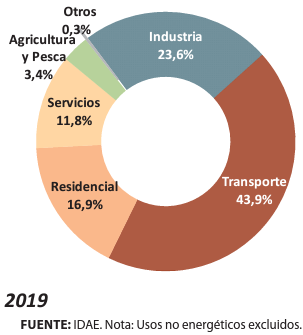
\includegraphics[width=\textwidth]{figuras/consumoEnergiaFinalPorSectores_2019}
		\caption{Consumo de energía por sectores.}
		\label{fig:consumoenergiafinalporsectores2019}
	\end{subfigure}
\caption[]{Desglose del consumo de energía primaria en España 2019 por fuente de energía(\subref{fig:fuentesenergiasprimarias}). Consumo de energía final por sectores en el año 2019 en España(\subref{fig:consumoenergiafinalporsectores2019}). \textit{Fuente:  Ministerio para la transición ecológica y el reto demográfico de España.} }
 \label{fig:consumosEnergiasCategorias}
\end{figure}

Para recuperar esta energía perdida se han desarrollado instalaciones de recuperación de calor residual, no solo para disminuir los costes sino también para disminuir las emisiones de contaminantes, cumpliendo así parte de los objetivos de desarrollo sostenible. El calor residual se puede aprovechar para obtener electricidad o para calentar un fluido para mejorar la eficiencia del mismo u otro proceso, disminuyendo el consumo de combustible u energía.\\

El aprovechamiento del calor residual para el calentamiento de otro fluido se utiliza en la industria, por ejemplo, un dispositivo llamado economizador que se usa en calderas para pre-calentar el fluido, mejorando el rendimiento térmico, o en el sector residencial que aprovecha el calor obtenido en el sistema de enfriamiento de algunos sistemas fotovoltaicos para obtener agua caliente.\\ 

La obtención de electricidad mediante el aprovechamiento del calor residual puede ser por vía de trabajo mecánico o por conversión directa. Por vía de trabajo mecánico se produce mediante ciclos termodinámicos, principalmente el ciclo de Rankine, el cual mediante un intercambiador de calor se genera vapor de agua que luego hace mover unas turbinas que están conectadas a un generador. La conversión directa se basa en la utilización de dispositivos termoeléctricos, termoiónicos, entre otros.\\

La conversión termo-eléctrica por vías mecánicas es la más conocida y es altamente utilizada, por ejemplo, las centrales nucleares, los sistemas de ciclos combinados, los sistemas de tratamientos de residuos que necesitan ser incinerados(figura \ref{fig:esquemaslomasvalorizacion}), entre otros. También se puede aprovechar el calor residual de la generación eléctrica, como es el caso de los cogeneradores.

%% IMAGENES DE SISTEMAS DE APROVECHAMIENTOS MECÁNICOS
\begin{figure}[H]
	\centering
	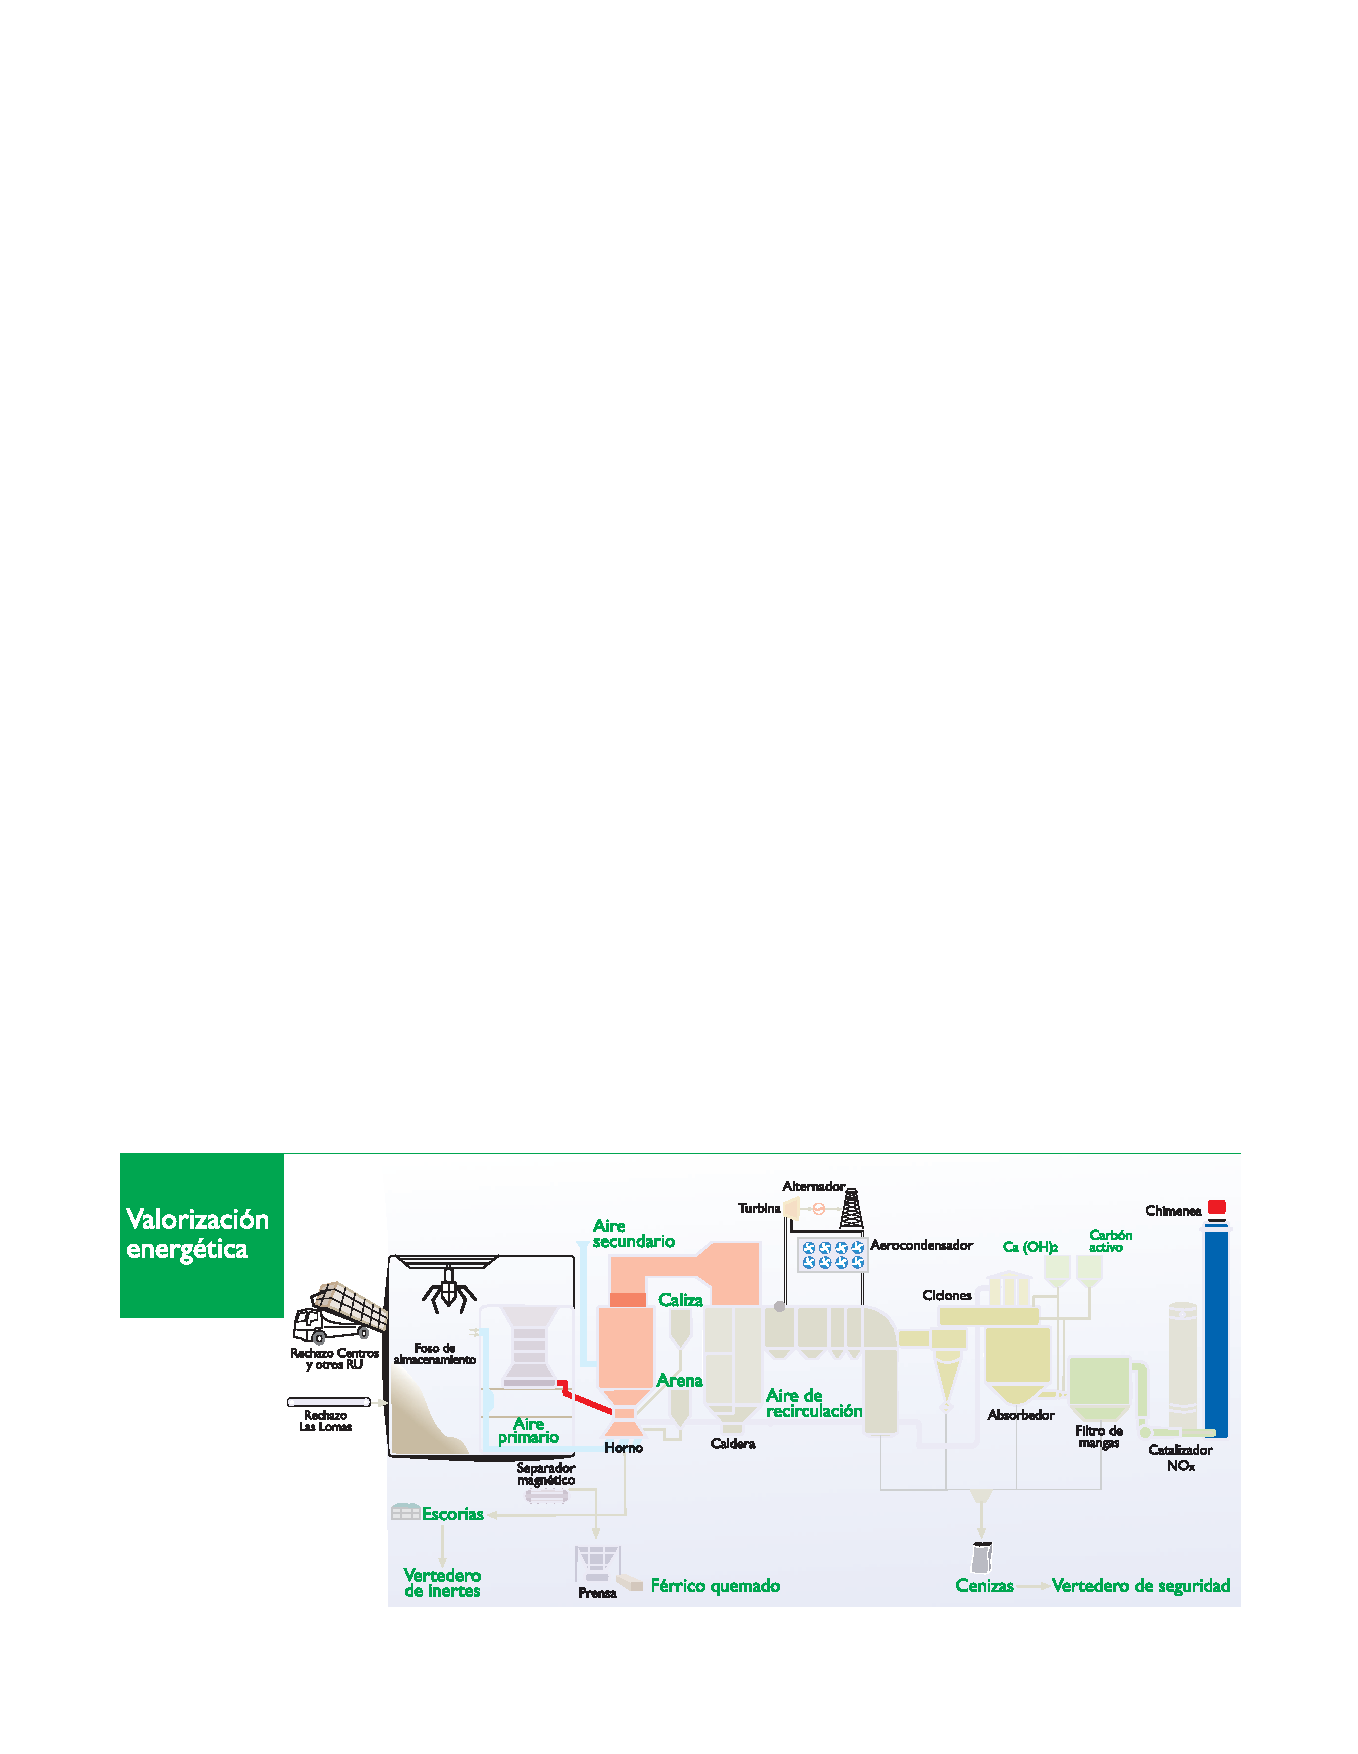
\includegraphics[height=5cm]{figuras/esquemasLomasValorizacion}
	\caption{Planta de valorización energética del Centro Las Lomas del Parque Tecnológico de Valdemingómez, donde se aprovecha los gases a alta temperatura para producir vapor de agua en la caldera para mover unas turbinas conectadas a generadores para producir electricidad. \textit{Fuente: Ayuntamiento de Madrid}}
	\label{fig:esquemaslomasvalorizacion}
\end{figure}

El problema principal con un sistema de este tipo son las partes móviles, las cuales tienen que estar en constante mantenimiento, para disminuir el mantenimiento se puede pasar a un sistema de recuperación de calor residual directo, ya sea con un dispositivo termoeléctrico, termoiónico o termofotovoltaico. Además de no presentar partes móviles o tener que tratar con fluidos, estos sistemas se pueden utilizar para varias aplicaciones, por ejemplo la espacial, donde la presión atmosférica es nula y la fuerza gravitacional total no es aproximadamente constante.\\

% Termo Electrico
Los dispositivos termoeléctricos son dispositivos semiconductores, uno tipo n y otro tipo p, que están unidos en sus extremos que cuando se les aplica una diferencia de temperatura entre ambas uniones, se genera una diferencia de potencial, conocido como efecto Seebeck, que se utiliza para generar electricidad. Los materiales que se utilizan para estos dispositivos tienen unas conductividades térmicas bajas, para disminuir las pérdidas por conducción de calor, y aumentar el coeficiente Seebeck del generador termo-eléctrico (TEG) porque a mayor sea esta diferencia, mayor será la diferencia de potencial.\\

La eficiencia de los TEGs es alrededor del 5\%, aunque hasta el momento la eficiencia ha llegado como máximo hasta aproximadamente 15\%, lo cual sigue siendo demasiado baja. Aún con bajas eficiencias los TEG se utilizan para aplicaciones espaciales, recuperación de calor en el transporte,entre otros.\\


% Termoiónico
Otros sistemas de obtención de electricidad de una fuente de calor es la generación termoiónica (TEC), que mediante el emisión termoiónica se produce un flujo de electrones entre el emisor metálico a alta temperatura y un receptor a menor temperatura, separados por el vacío. Al aumentar la temperatura del emisor, los electrones libres se excitan hasta tal punto que la energía es lo suficientemente grande como para que se desprendan del material, la densidad de corriente está determinada por la ley de Richardson, donde $J=A\cdot T^2\cdot e^{\frac{-W}{k\cdot T}}$, siendo J la densidad de corriente, A la constante de Richardson, W la función de trabajo del metal, k la constante de Boltzman y T la temperatura en Kelvin.\\

% Termofotovoltaico
Un generador que se puede utilizar en conjunto con el TEC, es un generador termofotovoltaico (TPV) que transforman la radiación electromagnética producida por el emisor a alta temperatura para ser capturada por el receptor, que es una célula fotovoltaica. Los emisores de las TPV no tienen que estar a unas temperaturas tan altas como los TEC, ya que no necesita que se desprendan los electrones. Ambos dispositivos presentan el mismo problema de pérdidas de electrones o fotones por los bordes del convertidor y para disminuir esto se disminuye la separación entre el emisor y el receptor. Cuando las distancias se vuelven nanométricas aumenta la transferencias de fotones por la transferencia de radiación evanescente y/o electrones por la eliminación del efecto de carga de espacio.\\

Los dispositivos que aprovechan los efectos de campo cercano presentan la dificultad de mantener la separación de manera constante por lo tanto se han fabricado y probado en varias ocasiones espaciadores de alturas desde un par de micras hasta unos pocos de cientos de nanómetros, con diferentes geometrías y materiales. Por ejemplo, en 


\section{Objetivos}
El objetivo de este estudio es diseñar y simular pilares de dimensiones nanométricas para el aprovechamiento del efecto de campo cercano en un convertidor termo-fotovoltaico, así como determinar la viabilidad de este sistema. 
\begin{itemize}
	\item Modelar un nano-espaciador dentro de los rangos permitidos de los parámetros de los programas de simulación y modelado 3D.
	\item Modelar el emisor y la célula del sistema TPV para que los gradientes térmicos por conducción no lleguen a los bordes.
	\item Simular la transferencia de calor por conducción a través de un nano-espaciador de $SiO_2$ de un sistema TPV para diferentes alturas del nano-espaciador, diferentes materiales de emisor y diferentes resistencias de contacto entre emisor y el nano-espaciador.
	\item Simular la transferencia de calor radiada entre el emisor y la célula para diferentes materiales del emisor y para varias distancias de separación, teniendo en cuenta los efectos de campo cercano en la radiación.
	\item Determinar entre los casos estudiados cuales pueden dar lugar a sistemas de TPV de campo cercano viables.
\end{itemize}


\section{Estructura del documento}

A continuación y para facilitar la lectura del documento, se detalla el contenido de cada capítulo.

\begin{itemize}
\item En el \textbf{capítulo 1} se realiza una introducción del trabajo con la respectiva motivación y objetivos.
\item En el \textbf{capítulo 2} se desarrolla el estado de arte, definiendo los apartados más importantes y resaltando las investigaciones con mayor relevancia.
\item En el \textbf{capítulo 3} se exponen las herramientas y materiales utilizados, así como los criterios de selección.
\item En el \textbf{capítulo 4} se mencionan los métodos seguidos y los cálculos realizados para el desarrollo del trabajo.
\item En el \textbf{capítulo 5} se exponen los resultados obtenidos de las simulaciones.
\item En el \textbf{capítulo 6} se desarrolla la conclusión y se realiza planteamientos para futuros trabajos.
\end{itemize}

  
  %partes finales del trabajo: conclusiones, bibliografia y anexos
  
\chapter{Estado del arte}
En este capítulo se exponen los principales temas de interés para la realización de este trabajo, las investigaciones realizadas sobre la TPV y NF-TPV (termofotovoltaica de campo cercano) y el marco teórico sobre las diferentes maneras que se transmite el calor.

\section{Termo-fotovoltaica}
%%%%%%%%%%%%%%   THERMO PHOTOVOLTAICA       %%%%%%%%%%%%%
Un generador termo-fotovoltaico(TPV) se basa en la conversión de energía calorífica en energía eléctrica mediante el efecto fotovoltaico a través una célula termo-fotovoltaica sin requerir ninguna parte móvil, conocido este tipo de sistemas de generación como motores pasivos de calor, como se representa de una manera sencilla en la figura \ref{fig:TPV_Subsistema}. El emisor se encuentra a una alta temperatura lo cual produce que se transmite el calor en forma de radiación que al llegar a la célula es reflejada, transmitida o absorbida, la porción de radiación absorbida excita a los electrones produciendo un par electrón-hueco sí solo sí la energía del fotón absorbido es mayor que la energía de la banda energética de la célula, al conectar los terminales de la célula a una carga se produce una corriente que alimenta a la carga proporcional a la intensidad lumínica, aquellos fotones con energía menor a la banda energética son suprimidos o reflejados para disminuir el flujo de calor\cite{Present_Efficiencies_and_Future_Opportunities_in_Thermophotovoltaics}.\\

\begin{figure}[H]
	\centering
	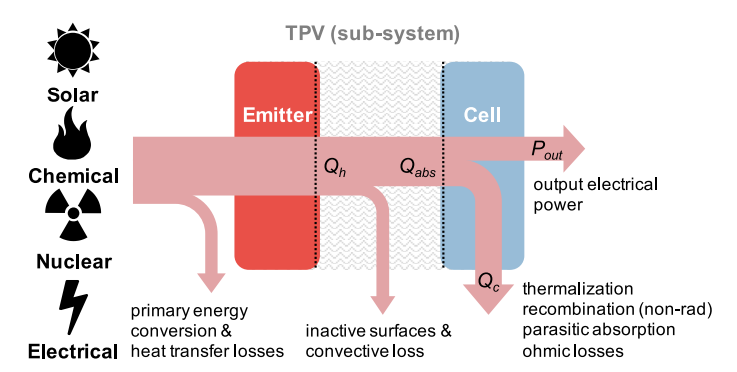
\includegraphics[width=0.7\textwidth]{figuras/TPV_Subsistema.png}
	\caption{Flujo de conversión de la energía térmica en energía eléctrica. \textit{Fuente: \cite{Present_Efficiencies_and_Future_Opportunities_in_Thermophotovoltaics}}}
	\label{fig:TPV_Subsistema}
\end{figure}

%%% INTERES EN LA TERMOFOTOVOLTAICA
La termofotovoltaica ha sido un campo de interés para aplicaciones militares, espaciales, generación de electricidad y recuperación de calor residual. Para la milicia de los Estados Unidos de América se han conducido varias investigaciones para la búsqueda de un generador eléctrico silencioso y portátil \cite{military_TPV}, cumpliéndose en 2004 40 años de investigación sin conseguirse potencias por encima de 500W \cite{military_TPV_40Years}. En aplicaciones espaciales es de interés por presentar beneficios en rendimiento para misiones cercanas al Sol y misiones en el espacio profundo porque los componentes más sensibles se encuentran resguardados de la dura radiación, siendo posible también el guardar energía en gravedad cero \cite{TPV_space_applications}. Para la recuperación de calor residual existe un gran interés porque la conversión de energía térmica a eléctrica es menor del 40\% en las plantas de generación de energía de combustibles fósiles convencionales, produciéndose una gran cantidad de pérdidas en forma de calor \cite{wasteHeat_TPV}.\\

%%% RESUMEN DE INVESTIGACIONES 
Todas estas áreas de interés ha provocado un aumento de las investigaciones en los sistemas de generación termo-fotovoltaicos, estudiándose la utilización de células multicapas, diferentes materiales de emisor para aumentar la potencia radiada, aplicación de capas finas en el emisor para el aumento de la potencia radiada\cite{doi:Near_field_ThinFilm}, aplicación de filtros \cite{multiLayerFilters} y capas reflectantes para la recuperación de fotones y disminución de calentamiento\cite{thermoionic_TPV_NF},la combinación con un TEC para aumentar la densidad de potencia y eficiencia total del sistema generador\cite{thermoionic_TPV_NF,progress_Thermoionic_TPV}, y la disminución del espacio entre emisor y célula para aprovechar los efectos de la radiación de campo cercano\cite{thermoionic_TPV_NF,modelEfficiency_NF_TPV,nf_TPV_Pillars_SiO2}.\\
%\cite{thermoionic_TPV_NF,modelEfficiency_NF_TPV,nf_TPV_Pillars_SiO2,NearField_200nm}

%%%  OTRA INVESTIGACIÓN 
Las investigaciones no se han limitado a estudiar células TPV de una o varias uniones p-n, sino también la utilización de células termofotovoltaicas interbandas en cascada (ICTPV) de banda energéticas comprendidas entre 0.2 y 0.5 eV que resulta en una eficiente colección de portadores foto-generados, donde la eficiencia máxima ($\eta_{max}$) y la diferencia de potencial en vacío ($V_{OC}$) es proporcional a el número de bandas (stages) hasta unos 0.691 V de $V_{OC}$ y uno 6.2\% $\eta_{max}$, pero genera una significante cantidad de energía térmica por la densidad de corriente oscura\cite{MultiEstados_Capas_TPVs}. Esta corriente se consigue disminuir al introducir una barrera entre las capas\cite{decreaseDarkCurrent}.\\

%%%  BACK SURFACE REFLECTOR AND FILTERS
Aún quedan por estudiar muchos materiales y disposiciones del emisor y de la célula, algo de alta importancia es el estudio de filtros y capas reflectantes porque permiten la re-utilización de los fotones no absorbidos, aumentando la eficiencia y evitando que se acabe calentando innecesariamente la célula. Las capas traseras reflectantes(BSR), principalmente hechas de oro, reducen las pérdidas de radiación por la absorción de la radiación de energía menor a la banda energética, permitiendo que la radiación vuelva al emisor \cite{nTPV_Review}. Habitualmente estas capas se usan en las TPVs y TICs, como por ejemplo se usan en \cite{thermoionic_TPV_NF,modelEfficiency_NF_TPV,thermophotovoltaic_40}. Los filtros se utilizan para evitar la transmisión de radiación no deseada  la célula, consiguiéndose un aumento de la eficiencia del 45\% al 75\%, estos filtros pueden ser de una o múltiples capas que la rugosidad de la interfaz degrada seriamente la eficiencia, lo que se puede mejorar con una poca cantidad de capas\cite{multiLayerFilters}.\\
%% Ahora va las investigaciones y poco a poco intercalando entre ellas

%%% DIFERENTES CERAMICAS
En \cite{differentEmitterCeramics} se estudian diferentes combinaciones de cerámicas para el emisor de una TPV a 2000\textdegree C y célula a 400\textdegree C, observando los flujos espectrales de calor, la potencia total y el rendimiento, siendo la máxima potencia por metro cuadrado para el emisor de $B_4C$ con unos 7.45 $Wm^{-2}$ pero solo con una eficiencia del 11.74\%, a diferencia del BeO con una potencia de 3.19 $Wm^{-2}$ y un rendimiento del 24.69\%. Y se observa como el rendimiento disminuye al disminuir la separación entre emisor y célula para luego volver a aumentar.\\

%%%  COMBINACION DE TPV CON TIC
La razón por la cual se combinan los TICs y las TPVs es para aprovechar tanto los electrones como los fotones radiadios, aumentando la densidad de potencia de salida y mejorando el rendimiento de una TPV. Si se disminuye la separación entre el emisor común y la célula por debajo de la micra se pasa a tener efectos de campo cercano, aumentando la potencia producida. En \cite{thermoionic_TPV_NF} utilizan un dispositivo termofotovoltaico de campo cercano mejorado con termoiónico (nTiPV) con un emisor de Tungsteno con una capa de $LaB_6$ a unos 2000K, que mejora el rendimiento de una TPV de un 10\% de eficiencia a un 30\% y un aumento de densidad de potencia de unos 10$Wm^{-2}$ a unos 70 $Wm^{-2}$ (figura \ref{fig:PowerDensityVSEfficiency_nTiPV}), por el uso de una célula sin mallado, disminuyendo la resistencia en serie y las pérdidas por sombras, utilizando un BSR para reflectar los fotones de baja energía.\\
\begin{figure}[H]
	\centering
		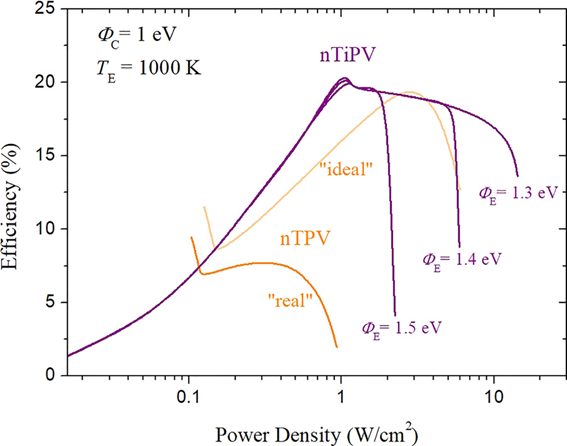
\includegraphics[height=7cm]{figuras/PowerDensityVSEfficiency_nTiPV.png}
	\caption{Relación entre densidad de potencia y eficiencia entre dispositivos nTPVs y nTiPVs. \textit{Fuente: \cite{thermoionic_TPV_NF}}}
	\label{fig:PowerDensityVSEfficiency_nTiPV}
\end{figure}

%%% CAMPO CERCANO
Los dispositivos TPV que aprovecha el efecto de campo cercano se denotan como dispositivos NFTPV, NF-TPV o nTPV, esto en combinación con el objetivo de disminuir la contaminación, aprovechar la energía desperdiciada en forma de calor y utilizar baterías más baratas con gran almacenamiento de energía ha impulsado bastante las investigaciones al respecto de la tecnología NF-TPV. Siendo el aumento de la eficiencia para igualar a la actual de campo lejano de 40\% \cite{thermophotovoltaic_40} un objetivo interesante, en \cite{modelEfficiency_NF_TPV} se modeló la eficiencia de un NF-TPV basado en InAs con emisor a  700K y radiador de la célula a 300K, alcanzándose unas eficiencia del 17\% siendo la separación de 200nm y notándose que a menores temperaturas y mayores distancias se obtiene menos potencia, y notando que al aumentar la temperatura el pico de potencia se desplaza a menores longitudes de onda.\\

%%% ECUACIONES
Dado que los costes de fabricación para el testeo pueden llegar a ser caros se utilizan modelos matemáticos para simular, siendo uno muy útil el presentado en \cite{nfTPV_equations} que proporciona varias ecuaciones para calcular la potencia radiada para varios grosores de emisor y receptor de una sola capa cada uno, siendo el de mayor utilidad el de capa gruesa que proporciona de una manera sencilla el cálculo de la potencia en un rango de longitudes de onda conociendo la función dieléctrica compleja de los materiales.\\

%%% FRECUENCIA DE RESONANCIA Y CAPAS FINAS PARA AUMENTO DE ENERGIA
Una ventaja que presenta los NF-TPV es la frecuencia de resonancia ($\omega_{res}$), que produce una mejora o aumento del flujo radiado a dicha frecuencia. En \cite{doi:Near_field_ThinFilm} utilizan una lámina fina de SiC y otra gruesa, obteniendo que al aumentar el grosor de la capa disminuye la potencia en la $\omega_{res}$ pero aumenta para el resto de frecuencias, siendo a partir de los 100nm de grosor la misma potencia radiativa que la lámina gruesa. Para mantener las distancias tan cortas es necesario un mecanismo, siendo lo más sencillo el uso de pilares de algún material cerámico por sus propiedades térmicas, como se presenta en \cite{NearField200} que estudia la transferencia de calor entre dos placas de Si separadas 200nm por vacío y utilizando espaciadores de SiO2 y prismáticos de base circular de 1 $\mu m$ de diámetro fabricados con fotolitografía ultravioleta, obteniéndose que el coeficiente radiativo de transferencia de calor aumenta con la disminución de la separación entre emisor y célula, y aumenta con la temperatura.\\

%%% RESISTENCIAS DE CONTACTO
También hay que tomar en cuenta la existencia de las resistencias de contacto entre cada interfaz, teniendo una gran importancia en \cite{nf_TPV_Pillars_SiO2} que estudia la radiación por campo cercano entre dos placas de cuarzo con pilares de pirámides truncadas de $SiO_2$ que están depositados sobre el substrato inferior, descubriéndose que la resistencia de contacto es mucho mayor que la geométrica del pilar, por lo tanto, es de gran importancia para disminuir las pérdidas por conducción.\\


\section{Transmisión de calor}
El calor es una forma de energía que se propaga entre distintos medios de tres formas distintas, por convección, radiación y conducción.
\subsection{Convección}
La transmisión de calor por convección se produce por la conducción de la energía cuando el fluido entra en contacto con el sólido y luego el transporte de la energía mediante el movimiento del fluido, pudiendo ser natural o forzada. La diferencia entre la convección natural y la forzada es la fuente de movimiento del fluido, en la convección forzada el movimiento del fluido es producido por una fuente externa, como un ventilador o una bomba, en la convección natural el fluido se mueve por las diferencias en densidades por la variación de la temperatura de partes del fluido.\\
\subsection{Radiación}
La radiación es la transmisión de energía térmica en forma de ondas electromagnéticas o fotones a través del vacío o un medio material proporcional a la temperatura del cuerpo del emisor. Cuando las ondas electromagnéticas inciden sobre la superficie de un material parte de ella es absorbida, otra parte reflejada y el resto se transmite internamente en el material, variando las proporciones de dichas cantidades según el material y la longitud de onda de la radiación. Existe dos flujos de radiación conocidos, el flujo de propagación o campo lejano y el flujo evanescente o campo cercano que excede los valores predichos por la Ley de Planck del cuerpo negro.\\

\subsubsection{Radiación propagación o campo lejano}
La radiación de campo lejano cumple la regla de Planck sobre la emitancia monocromática de un cuerpo negro (${E_{\lambda}}^{bb}(T)$) (ecuación \ref{eq:ecuacionPlanck}), cuyo valor total cumple con la Ley de Stefan Boltzmann (ecuación \ref{eq:leyDeStefanBoltzmann}) y el valor máximo cumple con la Ley de Wien, $\lambda_{max}\cdot T=2.896\cdot 10^3 \mu m\cdot K$, donde la temperatura (T) está en grados Kelvin.

\begin{equation}
{E_\lambda}^{bb}\left( T \right) = \dfrac{c_1\cdot \lambda^{-5}}{e^{\frac{c_2}{\lambda \cdot T}}-1}
\label{eq:ecuacionPlanck}
\end{equation}
\begin{equation}
{E}^{bb}\left( T \right)=\sigma \cdot T^4 \qquad \Longleftrightarrow \qquad \sigma = 5.67\cdot 10^{-8} \dfrac{W}{m^2 K^4}
\label{eq:leyDeStefanBoltzmann}
\end{equation}

 Pero las ecuaciones anteriores solo aplica para la radiación total emitida pero no la transferida entre dos superficies, siendo el caso más sencillo el de dos superficies planas, paralelas entre sí y de área infinita o mucho mayor que la distancia que las separa, donde la transferencia de calor entre ambas superficies consideradas como cuerpos grises se puede modelar como:
\begin{equation}
\frac{\Phi}{S}=\frac{\sigma \left( T_1^4 -T_2^4 \right)}{1/\epsilon_1 +1/\epsilon_2 -1}
\label{eq:flujoCalorSuperficiesGrises}
\end{equation}
Donde $\epsilon_i$ es la emisividad monocromática, es decir, el cociente de la emisividad del cuerpo respecto a la del cuerpo negro, cuyo vaor es constante por ser considerados las superficies como cuerpos grises.\\

Para la radiación de propagación en campo cercano se denota se resuelve de otra manera, que en el caso más sencillo el emisor y el receptor son cuerpos planos y gruesos, la ecuación que modela el flujo de calor por frecuencia de un emisor (nº1) a un receptor (nº3) separados por el vacío (nº2) es \cite{nfTPV_equations}:

\begin{equation}
q_{w,abs}^{prop}=\dfrac{\Theta \left( \omega,T_1 \right)}{4 \pi^2}\times \int^{k_\upsilon}_{0} k_\rho d\k_\rho \sum_{\gamma=TE,TM}\dfrac{\left( 1- \left| r_{21}^\gamma \right|^2\right) \left( 1-  \left| r_{23}^\gamma \right|^2 \right)}{\left| 1- r_{21}^\gamma r_{23}^\gamma e^{2ik_{z2}d_{c}} \right|^2}
\label{eq:flujoPropNF}
\end{equation}
Donde $\Theta \left( \omega,T_i \right)$ es la energía media de un oscilador de Planck para una frecuencia y temperatura dada, $r_{i,j}^\gamma$ es el coeficiente de reflexión de Fresnel en dicha interfaz en estado polarizado $\gamma$, TE son las ondas eléctricas transversales y TM son las ondas magnéticas transversales, i es la constante compleja $\sqrt{-1}$, $k_\rho$ es el vector de onda de la onda primaria \cite{nfTPV_fullEquations}.\\

La ecuación \ref{eq:flujoPropNF} es para dos placas gruesas separadas por un vacío y rodeadas por vacío, se obtiene de las ecuaciones presentadas en \cite{nfTPV_fullEquations}, donde se presenta las ecuaciones para la radiación de campo cercano de sistemas multicapa y un método numérico para solucionar las ecuaciones.

\subsubsection{Radiación evanescente o campo cercano}

\ref{eq:dos}
\begin{subequations}
\label{eq: uno}
\begin{equation}
\label{eq:dos}
  \operatorname{min}_{a,b,c} 
  \frac{1}{2}\mathbf{w}^{T}\mathbf{w} + C \sum_{i=1}^{l}\xi_{i} 
\end{equation}    
\begin{equation}
  y_{i}\left(\mathbf{w}^{T}\phi(x_{i})+b\right)
\end{equation}
\end{subequations}
\subsection{Conducción}
La transmisión de calor por conducción se dá a través de uno o varios cuerpos, producido por la diferencia de temperatura entre las caras opuestas del conjunto o cuando dos o más objetos a diferentes temperaturas entran en contacto. De manera genérica la conducción térmica se modela como $P_{cond}={\bigtriangleup T}/{R} $, siendo $R$ la resistencia térmica del sistema.
Para un solo material, la resistencia térmica se modela como $R = l/{\left(A\cdot h\right)}$, donde $l$ es la longitud del material, $A$ es la superficie y $h$ es la conductividad térmica del material. Para varios materiales colocados en serie, es decir, el flujo de calor que los atraviesa es el mismo para todos, la resistencia de conducción se define como la sumatoria de todas las resistencias de cada material($R=\sum R_i$).\\

En la realidad las interfaces de contacto entre los materiales no es perfecta, por ejemplo, la rugosidad de cada superficie, lo que provoca que haya una caída de temperatura entre cada interfaz, esta cada de temperatura se modela como una resistencia que se le llama resistencia de contacto.


\subsubsection{Resistencia de contacto}
La resistencia de contacto en la interfaz entre dos conductores produce una caída de temperatura significante, como se observa en el \cite{nf_TPV_Pillars_SiO2}, la cual es dependiente de muchos parámetros, tales como la temperatura, la presión, la rugosidad, etc.\\

Esta gran cantidad de dependencias hace que sea difícil parametrizar su valor, por lo tanto, se utilizan valores empíricos como el obtenido en \cite{nf_TPV_Pillars_SiO2} de unos $4E{-6} \ m^2K/W$, pero también se puede llegar a parametrizar para ciertos casos, como en \textbf{Otra citación}, donde modelan el cálculo de la resistencia de contacto entre dos aceros 304L a temperatura ambiente como $Modelo de resistencia de contacto$.

\chapter{Materiales y Herramientas}
%\vspace{-1cm}
En este capítulo se exponen los materiales utilizados para cada componente del sistema, las herramientas utilizadas para el modelado 3D del nano-espaciador, simulación de la transmisión de calor por conducción y simulación de transmisión de calor por radiación por campo cercano, y los motivos de uso de dichos materiales y herramientas.
\section{Materiales}
Se listan y desarrolla los materiales a utilizar para cada uno de los componentes del sistema TPV, incluyendo los criterios seguidos de su selección.
\subsection{Nano-espaciador}
El nano-espaciador es de Dióxido de Silicio ($SiO_2$), un material que ha sido utilizado en varias ocasiones en sistemas de campo cercano de TPVs o TEC por ser un material cerámico con una baja conductividad térmica, buena resistencia ante choques de calor y alta fuerza de compresión. La conductividad térmica es menor a 10 W/m\textdegree C en el rango de temperatura de trabajo, entre 25 a 800\textdegree C.\\

A su vez se considera el $SiO_2$ con tres porosidades distintas, la primera es con una porosidad del 0\%, segundo con una porosidad del 25\% y tercero con una porosidad del 50\%, calculando la nueva conductividad térmica para los casos de porosidad distinta al 0\% según el modelo CP en \cite{ThermalConductivity_SiO2_2018}.

\subsection{Célula}
La célula es en una primera instancia de Silicio (Si) para la realización de unas pruebas de simulación iniciales, se utiliza Silicio para dichas pruebas por ser muy conocido y utilizado en la fabricación de células fotovoltaicas. En el resto de simulaciones se utiliza Germanio (Ge), que es un semiconductor como el Si pero que es capaz de absorber una mayor cantidad de radiación por tener una banda energética (Band Gap) de 0.66eV a 300K, a diferencia del Si que es unos 1.11eV a 300K. La capacidad de absorber más radiación es importante en la termofotovolaica porque la mayor cantidad de radiación es infrarroja.\\

También se utiliza el Ge por ser el material de las células termofotovoltaicas a disposición en el Insituto de Energía Solar (IES).
\subsection{Emisor}
Para el emisor se utilizan Silicio, Acero inoxidable 304L (SS) y Carburo de Silicio (SiC). Se utilizá Si para las pruebas de simulación iniciales para tener un punto de partida, para luego pasar al \textit{SS} por ser un material que se utiliza mucho en la industria, incluyendo al transporte, y por último el SiC que es una cerámica que ha se ha utilizado para el aumento de potencia de radiación en campo cercano, aunque es mayor para una capa fina de SiC cercano a la frecuencia de resonancia \cite{doi:Near_field_ThinFilm}.\\\\
Se tomaron en cuenta otros materiales que han sido descartados por varias razones, entre ellas ser muy caros, tener baja potencia de radiación de campo cercano respecto a una célula de Ge, entre otros. %, similar conductividad térmica al SiC, Si o SS, punto de fusión menor o cercano a los 800\textdegree C, o por ser demasiado blandos. 
Dichos materiales son los siguientes:

\begin{itemize}
	\item \textbf{Antimoniuro de Galio (GaSb)}: Semiconductor con punto de fusión de 710\textdegree C que es menor a los 800\textdegree C que se encuentra el emisor, por lo cual no se puede utilizar porque empezará a pasar a estado líquido antes de llegar a la temperatura deseada.
	\item \textbf{Grafito}: es un material relativamente barato con una buena conductividad térmica, alto punto de fusión, pero es muy blando respecto al $SiO_2$, tiene como dureza máxima unos 50 HV (dureza Vickers) en comparación a la dureza del $SiO_2$ de unos 500 HV, por lo cual el nano-espaciador se hará paso por el emisor.
	\item \textbf{Tungsteno (W)}: El coste del material es medio, como máximo unos 56.4€/kg, su dureza Vickers es de unos 350 HV que es adecuada por no ser tan inferior a la del $SiO_2$, su conductividad térmica es más alta que la del nano-espaciador pero la potencia radiativa en campo cercano es baja, más cercana a la del acero.
	\item \textbf{Alumina ($Al_2O_3$)}: Es un material muy caro, aproximadamente 16000€/kg o más, disminuyendo considerablemente la viabilidad del sistema.
\end{itemize}

\section{Herramientas}

Los herramientas o programas utilizados durante el desarrollo del trabajo son variados y por diferentes motivos, a continuación se da una breve descripción y se explican los motivos de la utilización de cada programa.\\\\
Para la obtención de datos de los materiales se utilizan Granta EduPack 2021 R2, la página web Refractive Index y el resto de datos de los materiales que no se encuentren en dichas herramientas se obtienen de artículos de investigación. Para el modelado 3D se utiliza Autodesk Inventor 2021, para las simulaciones de la transmisión de calor por conducción se utiliza Autodesk CFD 2021, para la transmisión de calor por radiación se utiliza la Calculadora de campo cercano y para el análisis de datos se utiliza MATLAB.\\\\
Unas herramientas a destacar son TexStudio y TexnicCenter utilizadas para la redacción de este trabajo por la facilidad que presenta el escribir ecuaciones, actualizaciones de figuras y la menor necesidad de recursos que Word. También hay que destacar el uso de Git para el control de versiones del documento.\\
%%%  GRANTA EDUPACK 2021 R2
\subsection{Granta EduPack 2021 R2}
Programa desarrollado por la empresa Ansys que contiene varias bases de datos que recopila información sobre distintos materiales, teniendo un fácil acceso a la información básica de los mismos a través de una interfaz gráfica y estando organizadas de manera específica para cada base de datos. Este programa está disponible en la versión de Windows 10 del escritorio remoto de la UPM.\\\\
La base de datos utilizada es la \textit{Level 3} de las avanzadas porque recopila los datos de todos los materiales necesarios, en la mayoría de los casos incluye la variación de algunas propiedades respecto a la temperatura, siendo principalmente necesaria la conductividad térmica del material respecto a la temperatura.\\\\
Dado la gran cantidad de datos a disposición y la facilidad de obtención de los datos de los materiales, especialmente los datos que están disponibles con la variación de la temperatura, se utiliza este programa.
%%%   REFRACTIVE INDEX
\subsection{Refractive Index}
Esta página web (https://refractiveindex.info) recopila de artículos científicos los índices de refracción (n) e índices de extinción (k) de diferentes materiales en diferentes rangos de longitudes de onda, teniendo a disposición hipervínculos a los artículos de donde se extrajo los datos y la opción de descargar dichos datos.\\\\
El motivos de su utilización son la facilidad para la obtención de los índices de refracción y extinción, necesarios para los cálculos del flujo térmico de radiación por campo cercano, y la disponibilidad de los artículos utilizados para contrastar los valores presentados.

%\subsection{Modelado 3D}
%Para el modelado 3D de cada componente del sistema (emisor, célula y nano-espaciador) se utiliza Autodesk Inventor 2021 por la facilidades que presenta autoDesk de utilizar los archivos de un programa de la misma compañía en otro programa para continuar con el estudio del sistema.ç
%%%  Autodesk INVENTOR 2021
\subsection{Autodesk Inventor Professional 2021}
Es un software de Diseño 3D Asistido por Ordenador (CAD 3D) que ofrece herramientas para el diseño de piezas, ensamblajes, mecanismos, documentación y simulación de los sistemas. También permite el utilizar herramientas de entorno añadidas para simulaciones más complejas, el fácil acoplamiento para el uso de otros programas de Autodesk y el uso de parámetros en el diseño y modelado de las piezas.
\begin{figure}[H]
	\centering
		
\includegraphics[width=3cm]{figuras/inventorpro.png}
	\caption{Icono de Autodesk Inventor Professional 2021}
	\label{fig:inventorpro}
\end{figure}
Se utiliza el programa para el modelado 3D de los nano-espaciadores, el emisor, la célula y el sistema TPV completo. Los motivos de utilización del programa son:

\begin{itemize}
	\item Licencia estudiantil facilitada por la Universidad Politécnica de Madrid (UPM).
	\item Menor consumo de recursos que otros programas de modelado 3D.
	\item No necesita una conexión constante a internet para su uso.
	\item Acoplamiento con Autodesk CFD, permitiendo el lanzar modelos de Inventor a CFD. 
\end{itemize}

%\subsection{Simulaciones de transmisión de calor por conducción}
%Para la simulación de transmisión de calor se usa el programa Autodesk Computational Fluid Dynamics (CFD), que aún ser usado principalmente para simulaciones con fluidos también permite simular solo transmisión de calor por conducción en sólidos y permite usar los diseños de Autodesk Inventor para simular, siendo fácilmente creado el provecto de CFD desde Inventor en la pestaña nueva de simulación, que se crea automáticamente con la instalación de CFD, y haciendo click sobre \textit{Active Model Assessment Tool}. Usándose exclusivamente para las simulaciones de conducción porque no puede simular la transmisión de calor por campo cercano.
\subsection{Autodesk CFD}
Es un software desarrollado por Autodesk que se usa para crear simulaciones computacional de la dinámica de fluidos para la predicción del comportamiento complejo de fluidos (líquidos y gases), el programa también simula la transmisión de calor por conducción en sólidos, convección en fluidos y de radiación con la ayuda de un medio fluido. \\
\begin{figure}[H]
	\centering
		
\includegraphics[width=3cm]{figuras/CFD.png}
	\caption{Icono de Autodesk CFD}
	\label{fig:CFD}
\end{figure}
Se utiliza el programa para las simulaciones de transmisión de calor por conducción en vez de el entorno Nastran de Inventor por las siguientes razones:
\begin{itemize}
	\item Utilización de escalas pequeñas de los parámetros de los materiales.
	\item Fácil control del mallado.
	\item Control de los pasos de la simulación, la frecuencia de guardado de datos y el número de iteraciones.
	\item Fácil obtención de los datos de los flujos de calor y las temperaturas del espaciador en formato CSV.
	\item Obtención de un modelo de simulación desde Autodesk Inventor,
\end{itemize}

\subsection{MATLAB}
MATLAB es un programa o plataforma de programación de \textit{MathWorks} que permite desarrollar cálculos numéricos, desarrollar algoritmos, analizar datos y crear modelos matemáticos de sistemas para cálculo o simulaciones utilizando su propio lenguaje de programación. A su vez, MATLAB proporciona una tienda de paquetes donde los usuarios puede subir aplicaciones desarrolladas en MATLAB que permiten aprovechar aún más los recursos del sistema y facilitar el trabajo, ya sea analizar datos, obtener modelos matemáticos, entre otros.\\
\begin{figure}[H]
	\centering
		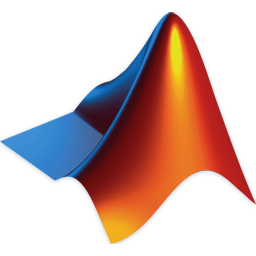
\includegraphics[width=3cm]{figuras/MatlabIcon.png}
	\caption{Icono de MATLAB}
	\label{fig:MatlabIcon}
\end{figure}
Se utiliza MATLAB para el análisis de los resultados obtenidos de las simulaciones de transmisión de calor por conducción y radiación, para realizar gráficas, para realizar cálculos y para desarrollar la aplicación de la calculadora de campo cercano. El principal motivo de usar MATLAB es porque el código principal de cálculo de transferencia de calor por radiación de campo cercano proporcionado está desarrollado en MATLAB.

\subsection{Calculadora de campo cercano}
Para las simulaciones de transmisión de calor por radiación de campo cercano entre dos placas paralelas de área infinita utilizando un código proporcionado que está escrito en MATLAB que cumple con las ecuaciones de campo cercano de \cite{nfTPV_equations} para dos placas planas gruesas y a partir de dicho código se desarrolla una aplicación en el App Designer de MATLAB para facilitar el proceso de calcular cualquier combinación de materiales para el emisor y la célula para ciertas distancias de separación.\\\\
Los motivos que impulsaron para desarrollar la aplicación son el simplificar el proceso de simular la radiación por campo cercano para diferentes combinaciones de materiales y distancia de separación, y la obtención de la potencia total para el rango de longitudes de onda deseadas para todas las combinaciones.\\

La aplicación se divide en tres pestañas \textit{Potencia Radiada}, \textit{Potencia} y \textit{Materiales}. En cuanto se abre la aplicación se presenta abierta la pestaña de \textit{Potencia Radiada}, donde se seleccionan los materiales del emisor y el receptor, las distancias de separación de los cuerpos y la temperatura del emisor, ya que la del receptor es fija a 300K y no influye en los cálculos. También muestra la gráfica de los resultados obtenidos de la simulación para cualquier combinación excepto cuando se eligen varios materiales y un rango de distancias.\\ 

\begin{figure}[H]
	\centering
		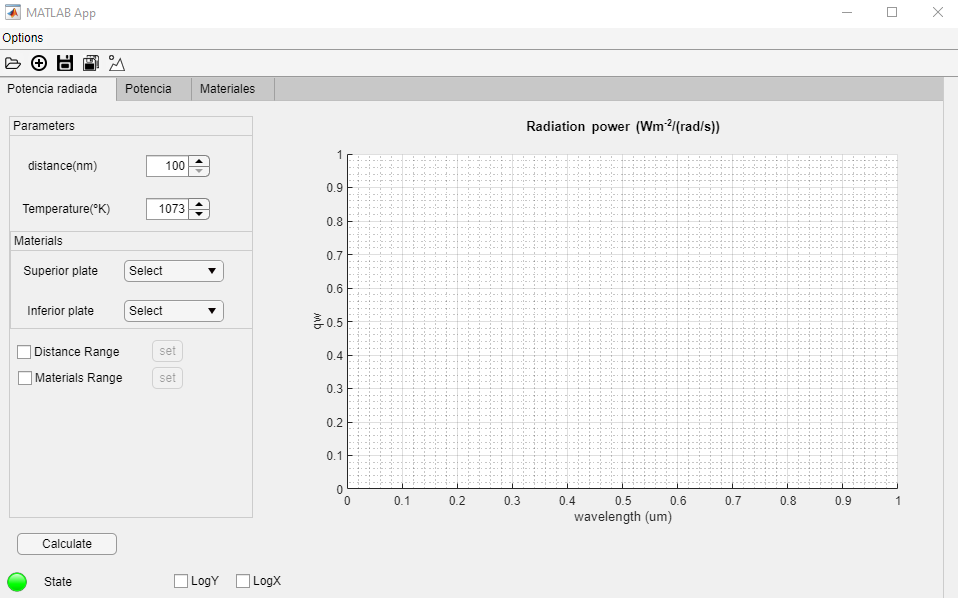
\includegraphics[width=0.80\textwidth]{figuras/pestana_PotenciaRadiada.png}
	\caption{Pestaña \textit{Potencia Radiada} de la calculadora de campo cercano}
	\label{fig:pestana_PotenciaRadiada}
\end{figure}

\begin{figure}[H]%
\centering
\begin{subfigure}[b]{0.48\textwidth}
\centering
	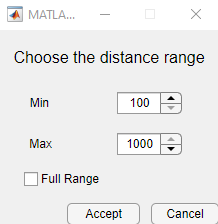
\includegraphics[width=0.8\textwidth]{figuras/pestana_Distancias.png}
	\caption{Ventana de selección de rango de distancias}%
	\label{fig:ventana_dist}%
\end{subfigure}
\hfill
\begin{subfigure}[b]{0.48\textwidth}
\centering
	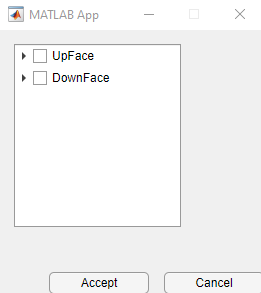
\includegraphics[width=0.8\textwidth]{figuras/pestana_Elegirmateriales.png}
	\caption{Ventana de selección de materiales}%
	\label{fig:ventana_mat}%
\end{subfigure}
\caption{(\subref{fig:ventana_dist}) Ventana para la selección del rango de las distancias de separación entre el emisor y el receptor. (\subref{fig:ventana_mat}) Ventana para la selección de los materiales para el emisor y el receptor.}%
\label{fig:ventanas_d_mat}%
\end{figure}
Cabe destacar que la aplicación sigue en fase de desarrollo, todavía no se ha terminado de agregar todas las funcionalidades y arreglar los bugs.

\chapter{Métodos}\label{chapter:Metodos}
En este capítulo se detallan los criterios seguidos para la elección de la geometría de los espaciadores y su escala, los cálculos realizados para adaptar las propiedades de los materiales a las limitaciones de escala de los programas de simulación, los procedimientos seguidos para realizar las simulaciones y el procedimiento seguido para la extracción de los datos de la simulación de CFD.
\section{Criterios de geometría y escala}
Los criterios de geometría y escala se basan principalmente en el proceso de fabricación de los nano-espaciadores por fotolitografía, que es la técnica que se utilizará en el desarrollo de los primeros experimentos que intentarán corroborar los resultados obtenidos en este trabajo de simulación, esto en una siguiente etapa de la investigación.\\\\
La base del nano-espaciador es cuadrada por ser la geometría más sencilla de fabricar mediante procesos fotolitográficos y para realizar cálculos, por ser sus ecuaciones de área y volumen las más sencilla de los polígonos regulares cerrados. El lado de la base del nano-espaciador son de 3 $\mu m$ por ser el límite de resolución de la mayoría de equipos de fotolitografía, es decir, es la mínima distancia que se puede definir mediante fotolitografía.\\\\
Se utiliza 100 nm como la distancia mínima para definir la altura mínima de los nano-espaciadores, correspondiente a 1 mm de la escala del modelo 3D en Inventor. Por lo tanto, el factor de escala que se aplica a las unidades de longitud es $10^4$, que se toma en cuenta a la hora de definir las propiedades térmicas que involucren unidades de longitud, como es la conductividad térmica ($W/m2$).
%%% CALCULOS DE LAS PROPIEDADES DE LOS MATERIALES
\section{Cálculos de las propiedades de los materiales para las simulaciones}
Para obtener los nuevos parámetros de distancias, áreas y volúmenes del modelo 3D del nano-espaciador se procede a obtener las relaciones de escala entre el modelo y la realidad. También se obtienen las relaciones de las propiedades más significativas de los materiales de la realidad y las simulaciones de transmisión de calor por conducción, siendo la principal propiedad la conductividad térmica. Otras propiedades que se toman en cuenta son la densidad y el calor específico, teniendo que destacar la resistencia de contacto por unidad de área entre el nano-espaciador y el emisor.\\\\
Para diferenciar las dimensiones reales de las dimensiones utilizadas en el modelo 3D se utilizará el apostrofe después de la variable correspondiente, por ejemplo, para la longitud real se usa $L$ y para la longitud en el modelo 3D se usa $L'$.\\\\
La relación de longitudes entre el modelo 3D y la realidad es:
\begin{equation}
{L'}/{L}={1mm}/{100nm}=10^4
\label{eq:relacion_longitud}
\end{equation}
%%%  AREA
\subsection{Área}
La sección de los nano-espaciadores es un cuadrado cuya fórmula de área es $A=L^2$, donde $A$ es el área y $L$ el lado del cuadrado, siendo la relación de las áreas la siguiente:
\begin{equation}
	\dfrac{A'}{A}=\left(\dfrac{L'}{L}\right)^2=10^8
	\label{eq:relacion_areas}
\end{equation}
%%% VOLUMEN
\subsection{Volumen}
El volumen de un prisma de base cuadrada se expresa como $V=A\cdot L$, donde $L$ es la altura del prisma.
\begin{equation}
	\dfrac{V'}{V}=\dfrac{A'\cdot L'}{A\cdot L} = 
	\dfrac{A'}{A}\cdot \dfrac{L'}{L} \ \Longrightarrow \ \dfrac{V'}{V} =10^{12}
	\label{eq:relacion_volumen}
\end{equation}
El volumen de cada nano-espaciador en el modelo será $10^{12}$ veces el volumen original.
%%% DENSIDAD
\subsection{Densidad}
La masa de cada elemento es igual entre el modelo($M'$) y la realidad($M$), por lo tanto la densidad varía.
\begin{equation}
\dfrac{\rho '}{\rho}=\dfrac{M'/V'}{M/V}=\dfrac{M'}{M}\cdot \dfrac{V}{V'} \ \Longrightarrow \ 
\dfrac{\rho '}{\rho}=10^{-12}
\label{eq:relacion_densidad}
\end{equation}
La densidad de cada elemento en el modelo será $10^{-12}$ veces la densidad de la realidad.
%%% CONDUCTIVIDAD TERMICA
\subsection{Conductividad Térmica}
La resistencia térmica de los materiales del modelo de simulación se mantiene igual a la de la realidad, por lo tanto, la conductividad térmica de los materiales en el modelo son distintas a la realidad. Sabiendo que la fórmula de la resistencia térmica de conducción es $R=1/k \cdot L/A$, donde $k$ es la conductividad térmica, $L$ la longitud y $A$ es la sección, se puede obtener la relación de las conductividades térmicas del modelo de simulación respecto a la realidad.
\[ \dfrac{R}{R'}= \dfrac{1/k}{1/k'}\cdot \dfrac{L/A}{L'/A'}= \dfrac{k'}{k}\cdot \dfrac{L}{L'}\cdot \dfrac{A'}{A}=1\]
\begin{equation}
\dfrac{k'}{k}=\dfrac{L'}{L}\cdot \dfrac{A}{A'}=\dfrac{10^4}{10^8} \ \Longrightarrow \ \dfrac{k'}{k}=10^{-4}
\label{eq:relacion_conductividadTermica}
\end{equation}
Para el caso del nano-espaciador de $SiO_2$ que puede presentar diferentes porosidades para el material, se multiplica la conductividad térmica por la conductividad térmica normalizada para dicha porosidad \cite{ThermalConductivity_SiO2_2018}.
%%% CALOR ESPECIFICO
\subsection{Calor Específico}
El calor específico de los materiales del modelo de simulación es el mismo que el de la realidad porque el calor específico se define como la cantidad de calor necesaria que hay que suministrar a una unidad de masa para elevar su temperatura en una unidad, como la masa del modelo de simulación es igual a la de la realidad, la cantidad de energía necesaria para elevar una unidad de temperatura va a ser igual al del modelo de simulación respecto a la realidad, por lo tanto, el calor específico se mantiene igual al de la realidad.
%%% RESISTENCIA DE CONTACTO
\subsection{Resistencia de contacto}\label{sec:metodos_Rc}
La resistencia de contacto ($R_c$) es difícil de modelar matemáticamente en una ecuación ya que depende de muchas variables, como la temperatura, presión, entre otros. La resistencia de térmica producida por la resistencia de contacto es $R_{th}=R_{c}/A$, donde A es la superficie de contacto, por lo tanto se ve afectado por la diferencia de escala entre el modelo de simulación y la realidad.
\[ \dfrac{R_{th}'}{R_{th}}=\dfrac{R_c'}{R_c}\cdot \dfrac{A}{A'}=1 \]
\begin{equation}
	\dfrac{R_{th}'}{R_{th}}=\dfrac{R_c'}{R_c}\cdot \dfrac{A}{A'}=1 \ \Longrightarrow \  \dfrac{R_c'}{R_c}=\dfrac{A'}{A}=10^8
	\label{eq:relacion_Rc}
\end{equation}
%%% YOVANOVICH
De la literatura, solo se encontró en \cite{experimental_Rc_SS} expresiones analíticas para calcular la conductancia de contacto (\gls{hc}) entre dos superficies, las cuales han sido validadas para el caso concreto de dos superficies de SS. Pudiéndose obtener la $R_c'$ aplicando la inversa a la $h_c$ del modelo ($h_c'$).\\\\
Estas expresiones analíticas solo se aplicarán al modelo de simulación de la nTPV de emisor de SS, es decir, nTPV de $SS-SiO_2-Ge$, que para la obtención de la $h_c'$, y por ende la $R_c'$, se relacionan la $h_c'$ con la $h_c$ del caso concreto de SS \cite{experimental_Rc_SS}. Para obtener esta relación, simplificamos las ecuaciones suponiendo que el nano-espaciador de $SiO_2$ es liso, por ende, su pendiente media de la rugosidad ($m_i$) y su rugosidad ($\sigma_i$) son nulas.\\\\
La \gls{hc} se obtiene según un modelo matemático presentado en \cite{experimental_Rc_SS} y según la ecuación de Cooper reducida por Yovanovich (ecuación \eqref{eq:ecuacionesRcYovanovich}).\\
\begin{equation}
\dfrac{h_c\sigma}{k_sm}=1.25\left(\dfrac{P}{H_c}\right)^{0.95}
\label{eq:ecuacionesRcYovanovich}
\end{equation}
Donde $\sigma$ es la combinación RMS de la rugosidad de ambas superficies de los materiales, que está definida en la ecuación \eqref{eq:sigmaRMS}, $m$ es la combinación RMS de la media absoluta de la pendiente de la rugosidad, definida en la ecuación \eqref{eq:mRMS}, $k_s$ es la media armónica de la conductividad térmica, cuya ecuación está definida en la ecuación \eqref{eq:condArmonica}, $H_c$ es la micro-dureza Vickers del material más duro y \gls{p} es la presión aplicada.\\
\begin{subequations}
\begin{minipage}{0.298\textwidth}
\begin{equation}
m=\sqrt{m_1^2+m_2^2}
\label{eq:mRMS}
\end{equation}
\end{minipage}
\hfill
\begin{minipage}{0.28\textwidth}
\begin{equation}
\sigma=\sqrt{\sigma_1^2+\sigma_2^2}
\label{eq:sigmaRMS}
\end{equation}
\end{minipage}
\hfill
\begin{minipage}{0.28\textwidth}
\begin{equation}
k_s=2\cdot \frac{k_1\cdot k_2}{k_1+k_2}
\label{eq:condArmonica}
\end{equation}
\end{minipage}
\label{eqs:RMS}
\end{subequations}


La presión de contacto adimensional, es decir, la relación entre la \gls{p} y la $H_c$ de la ecuación \eqref{eq:ecuacionesRcYovanovich}, se obtiene a partir del modelo propuesto por Song y Yovanovich, recopilados en \cite{experimental_Rc_SS}, según la ecuación \eqref{eq:modeloYovanovich} donde $c_1$ es 10.6 GPa y $c_2$ es -0.40.
\begin{equation}
\dfrac{P}{H_c}=\left[ \dfrac{P}{c_1\left(1.62\sigma/m\right)^{c_2}} \right]^{\frac{1}{2+0.071c_2}}
\label{eq:modeloYovanovich}
\end{equation}

%% Valores de las constantes
Como se puede observar en las ecuaciones \ref{eq:ecuacionesRcYovanovich} y \ref{eq:modeloYovanovich}, el valor de $\sigma$ y $m$ se presentan siempre relacionados como $\sigma / m$, y se cumple que $\sigma /m =\sigma ' / m'$ porque al suponer que el caso de dos aceros tienen idénticas $m_i$ y $\sigma_i$, la relación $\sigma / m$ queda como $\sigma_i / m_i$, que resulta ser la misma relación para el caso de SS-$SiO_2$.\\\\
\[ \frac{\sigma}{m}=\frac{\sqrt{\sigma_{SS}^2+\sigma_{SS}^2}}{\sqrt{m_{SS}^2+m_{SS}^2}}=\frac{\sigma_{SS}\sqrt{2}}{m_{SS}\sqrt{2}} =\frac{\sigma_{SS}}{m_{SS}}\]
\[ \frac{\sigma'}{m'}=\frac{\sqrt{\sigma_{SS}^2+0^2}}{\sqrt{m_{SS}^2+0^2}}=\frac{\sigma_{SS}}{m_{SS}} \]
%%%%%%
Por lo tanto, considerando que $c_1$ y $c_2$ no varían con el cambio de material, la relación de $h_c'$ respecto a \gls{hc} se obtiene relacionando la ecuación \eqref{eq:ecuacionesRcYovanovich} del modelo a simular con la realidad.
%%%%
\[Cte=1.25\frac{m}{\sigma}\cdot \left(\dfrac{P}{H_c}\right)^{0.95} \qquad \Longrightarrow \qquad h_c=k_s\cdot Cte\]
%%
Donde $Cte$ es una constante que es igual para el caso de los aceros, como para el caso SS-$SiO_2$. El valor de $k_s$ para el caso de de los aceros es $k_{SS}$, siendo $k_{SS}$ la conductividad térmica del \acrshort{ss}. 
%%
\[ \frac{h_c'}{h_c}=\frac{k_s'}{k_s}\cdot \frac{Cte}{Cte}=\frac{2 \cdot \frac{k_{SS}\cdot k_{SiO_2}}{k_{SS}+k_{SiO_2}}}{k_{SS}}\]
\begin{equation}
\frac{h_c'}{h_c}=2\cdot \frac{k_{SiO_2}}{k_{SS}+k_{SiO_2}}
\label{eq:relacion_conductividadesTermicas}
\end{equation}
Para este trabajo los datos utilizados de las conductividades térmicas de los materiales para la relación de las conductancias de contacto son a temperatura ambiente, el valor de $k_{SiO_2}$ es $1.5 \ W/\left( m^2 K\right)$ y el valor de $k_{SS}$ es de $15 \ W/\left( m^2 K\right)$, quedando la relación de conductancias de contacto como ${h_c'}/{h_c}=0.1818$.
\vfill
%%%%%%%%     PROCEDIMIENTOS DE LAS SIMULACIONES Y EXTRACCION DE RESULTADOS
\section{Procedimientos de las simulaciones y extracción de resultados}
A continuación se describen los procedimientos seguidos en este trabajo para la realización de la simulación de la transmisión de calor por radiación de campo cercano, la simulación de la transmisión de calor por conducción y la extracción de los datos de las simulaciones.\\
\subsection{Para la radiación de campo cercano}
%Aquí tendrías que meter las simulaciones de campo cercano y hablar del método (está descrito en un paper que te pasé
Las simulaciones de transmisión de calor por radiación de campo cercano se realizan para una combinación de varios materiales de emisor y célula en un rango de distancias de 100 nm a 1000 nm. Para la realización de las simulaciones y la obtención de la potencia se siguen los pasos detallados en el apéndice \ref{ch:procedimientosSimRad}. A continuación se expone un procedimiento simplificado para la realización de una simulación.
\begin{enumerate}
	\item Abrir la aplicación de la Calculadora de campo cercano.
	\item Seleccionar los materiales para el emisor y el receptor que se desean simular. 
	\item Seleccionar el rango de distancias de separación deseado.
	\item Asegurar que la temperatura del emisor sea la deseada.
	\item Ejecutar la simulación y esperar a que termine.
	\item Seleccionar el rango espectral de integración de las potencias frente a la longitud de onda.
	\item Integrar y graficar los resultados de la integración.
	\item Guardar los resultados de la potencia integrada.
\end{enumerate}
%%%%%%%%%%%%%%%%%%%%%%%%%%%%%%%%%%%%%%%%%
%%%%%%%%%%%%     Conducción térmica
%%%%%%%%%%%%%%%%%
\subsection{Para la conducción térmica}
Las simulaciones de transmisión de calor por conducción se realizaron todas en CFD, existiendo unos 10 casos para cada combinación de materiales y resistencias de contacto, para cada uno de ellos se sigue un mismo conjunto de pasos. \\\\
Primero hay que crear el modelo 3D de cada componente del sistema TPV a simular, siendo cada uno de ellos es un prisma de sección cuadrada. El nano-espaciador tiene de base un cuadrado de lado 3 $\mu m$ y de altura variable $h$, el emisor y la célula tiene el mismo modelo 3D, con base cuadrada de 1 mm de lado con 0.2 mm de altura. Para el cálculo de las longitudes del modelo 3D se utiliza la ecuación \eqref{eq:relacion_longitud}.
%%%%%%%%%%%%%%%%%%%%%%%%%%
%%% MODELADO 3D
\subsubsection{Procedimiento modelado 3D}
El procedimiento seguido para la obtención de los modelos 3D en Inventor y la creación del modelo de simulación inicial para cada altura del nano-espaciador está detallado paso a paso en el apéndice \ref{ch:procedimientosModelado3D}. A continuación se expone un procedimiento genérico para la creación de los modelos 3D.
\begin{enumerate}
	\item Crear las bases cuadradas con la longitud de lado respectiva, 10 m para emisor o célula y 3 cm para el nano-espaciador en la escala del modelo 3D en Inventor. 
	\item Extrudir el prisma la longitud correspondiente, 2 m para los emisor/célula y 1 mm para el nano-espaciador.
	\item Crear un ensamblaje de emisor-espaciador-célula, estando la base del nano-espaciador en el centro de las bases de los otros dos componentes, como se observa en las figuras \ref{fig:modelado3D1} \subref{fig:modelado3D_cerca1} y \subref{fig:modelado3D_centro_cerca1}.
\begin{figure}[H]
	\centering
	\begin{subfigure}[b]{0.4\textwidth}
		\centering
			
\includegraphics[width=1.00\textwidth]{figuras/Procedimiento_Simulaciones/Conduccion/modelado3D_cerca.png}
		\caption{Vista cerca TPV}
		\label{fig:modelado3D_cerca1}
	\end{subfigure}
	\hfill
	\begin{subfigure}[b]{0.4\textwidth}
		\centering
			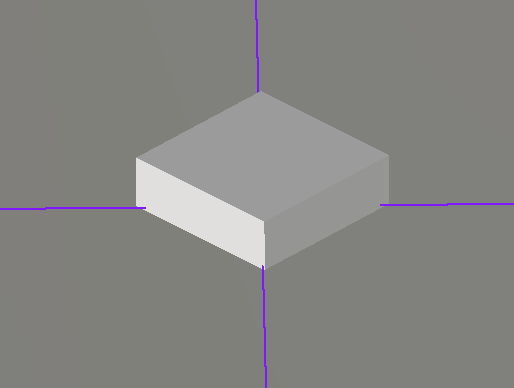
\includegraphics[width=1.00\textwidth]{figuras/Procedimiento_Simulaciones/Conduccion/modelado3D_centro_cerca.png}
		\caption{Vista cerca nano-espaciador}
		\label{fig:modelado3D_centro_cerca1}
	\end{subfigure}
	\caption{Vistas del sistema TPV. (\subref{fig:modelado3D_cerca}) Vista del sistema TPV de cerca desde un borde. (\subref{fig:modelado3D_centro_cerca}) Vista del nano-espaciador colocado sobre el centro de una cara de la célula.}
	\label{fig:modelado3D1}
\end{figure}
	\item Usar la herramienta \textbf{Active Model Assessment Tool}, que se encuentra en la pestaña de simulaciones, para generar el modelo de simulación de CFD\label{itm:pasoIniIterativo_Modelado3D1}.
	\item Guardar el modelo de CFD y volver al ensamblado de Inventor.
	\item Incrementar la altura del modelo del nano-espaciador un milímetro dentro del ensamblaje en Inventor, sin sobrepasar el máximo de 10 mm.
	\item Repetir todo 10 veces desde el paso \ref{itm:pasoIniIterativo_Modelado3D1}, teniendo como última iteración el modelo de la TPV con nano-espaciador de 10 mm, equivalente a 1 $\mu m$ de la realidad.
\end{enumerate} 

%%%%%%%%%%%%%%%%%%%%%%%%%%%%%%%%%%%%%%%%%%%
%   Procedimiento simulación CFD
\subsubsection{Procedimiento simulación CFD}
%%%  PROCEDIMIENTO CFD
El procedimiento a seguir para cada modelo de la simulación de transmisión de calor por conducción en CFD está detallado en el apéndice  \ref{ch:procedimientosSimCond}. A continuación se expone un procedimiento sencillo sobre la realización de las simulaciones en CFD.
\begin{enumerate}
	\item Abrir el modelo o estudio correspondiente de simulación en CFD.
	\item Aplicar los materiales adecuados para cada componente con la propiedad de entorno puesta en \textit{variable}.
	\item Aplicar en caso que aplique la resistencia de contacto sobre la superficie superior del nano-espaciador.
	\item Aplicar las condiciones de contorno a los componentes del sistema, es decir, las temperaturas al emisor y a la célula.
	\item Aplicar un mallado apropiado para cada componente del sistema, teniendo el nano-espaciador una gran cantidad de nodos.
	\item Simular la transmisión de calor en el modo estacionario hasta llegar al régimen estacionario.
	\item Extraer o guardar los resultados de las potencias de conducción en un CSV.
	\item Repetir estos pasos para cada modelo con distintas alturas de nano-espaciadores.
\end{enumerate}

%\chapter{Cómo escribir en Latex}

\section{Citas}

%las referencias a artículos se ponen con \cite, 
%las referencias a imágenes \ref, 
%y las referencias a ecuaciones \eqref

Esto es un ejemplo de cita de un artículo %\cite{Brunete:2013}.


\section{Listas}

%itemize es una lista. Cada término lleva delante un \item
Ejemplo de lista de puntos:
\begin{itemize}
\item Ejemplo1.
\item Ejemplo2.
\end{itemize} 

Y lista numerada:
\begin{enumerate}
\item Elemento 1
\item Elemento 2
\end{enumerate}

\section{Tablas}

Ejemplo de tabla. Como se aprecia en la tabla \ref{tab:table_example}...
\begin{table}[tb]
\caption{Ejemplo de tabla}
\label{tab:table_example}
\begin{center}
\begin{tabular}{|c||c|c|}
\hline
One & Two & Three\\
\hline
F1A & F1B & F1C\\
F2A & F2B & F2C\\
\hline
\end{tabular}
\end{center}
\end{table}

\section{Referencia a una sección}
\label{sec:refsec}

Ejemplo de referencia a la sección \ref{sec:refsec}

\section{Texto}

Testo en \textbf{negrita} y \textit{cursiva}.

\section{Figuras}

Ejemplo de referencia a figura (figura \ref{fig:logo_upm}). Es importante que todas las figuras que aparezcan estén referenciadas, así como las tablas. En general las figuras se colocarán al principio o al final de cada página ([tb] en latex), a no ser que por alguna necesidad se deban colocar en una posición exacta ([h]).

%caption es el pie de foto, y label es el nombre que se da a la imagen para referenciarla después. label no puede llevar acentos y no se muestra de cara al documento final (es sólo interno).
\begin{figure}[tb]
\centering

\includegraphics[width=0.45\textwidth]{figuras/Logo_UPM.jpg}   
\caption{Logotipo de la UPM}
\label{fig:logo_upm}
\end{figure}

\chapter{Resultados y discusión}
En este capítulo se presentan las relaciones entre la cantidad de potencia transmitida por radiación (que es una potencia aprovechable para generar electricidad) y la cantidad de potencia transmitida por conducción (la cual no se puede aprovechar) para diferentes combinaciones de materiales de emisor y célula.\\\\
Para determinar estas relaciones se simula la transmisión de calor por conducción a través de un nano-espaciador, para luego extrapolar la cantidad de calor por conducción que se obtendría para un dispositivo de 1 $cm^2$ con distintas distribuciones de nano-espaciadores ($n^{\underline{\circ}}\ espaciadores/cm^2$, y se simula la transmisión de calor por radiación de campo cercano en un dispositivo de 1 $cm^2$. Las simulaciones se realizan con el emisor a una temperatura constante de 800\textdegree C y la célula a 25\textdegree C.
\begin{itemize}
	\item Primero se valida la simulación de CFD.
	\item Se presentan los resultados de las simulaciones de transmisión de calor por conducción y por radiación de campo cercano para diferentes combinaciones de materiales de emisor y célula, y la relación entre ambas simulaciones.
	\item Se estudia el número mínimo de espaciadores necesarios para soportar la carga de los emisores.
	\item Por último, se presentan los resultados de usar un nano-espaciador de $Si$ en vez de $SiO_2$ para emisores de $Si$ y $SS$.
\end{itemize}
%%%%%%%%%%%%%%%%%%%%%%%%%%%%%%%%%%%%%%%%%%%%%%%%%%%%%%%%%%%%%%%%%%%%%%%
%% COMPROBACIÓN DEL PROCEDIMIENTO DE EXTRACCIÓN DE RESULTADOS DE CFD
%%%%%%%%%%%%%%%%%%%%%%%%%%%%%%%%%%%%%%%%%%%%%%%%%%%%%%%%%%%%%%%%%%%%%%%
\section{Validación de las simulaciones de CFD} \label{sec:val_CFD}
Las simulaciones de CFD son validas al comprobarse que con ellas se obtienen los mismos resultados que el modelo analítico (ecuación \eqref{eq:conduccion}) cuando se imponen las mismas simplificaciones de dicho modelo, es decir, cuando se impone una conductividad térmica constante y altura del nano-espaciador de 1000 nm.
\begin{equation}
Q=k\cdot \Delta T
\label{eq:conduccion}
\end{equation}
Para simplificar suponemos que la conductividad térmica ($k$) de los materiales es constante con la variación de la temperatura y usamos su valor para una temperatura de 25 \textdegree C, la $k$ del $Si$ es 182.98 W/m\textdegree C y la del $SiO_2$ es 1.30 W/m\textdegree C. De la simulación se extrae el flujo de calor del sistema y la temperatura media máxima y mínima de las superficies de contacto del nano-espaciador con los otros componentes del sistema.\\\\
La temperatura media máxima del nano-espaciador es 792.601\textdegree C, la temperatura media mínima del nano-espaciador es 32.39\textdegree C y el flujo de calor es 8897.93 $\mu W$. Con los resultados de las temperaturas medias del nano-espaciador se obtiene un flujo de calor teórico de 8899.05 $\mu W$ (obtenido mediante la ecuación \eqref{eq:conduccion}, siendo $k$ la conductancia térmica $k=\sigma \cdot A/L$), obteniéndose un error relativo aproximado del $12.6\cdot 10^{-3}$\%, por lo tanto el procedimiento es apropiado para la obtención de los resultados de las simulaciones de transmisión de calor por conducción.
%%%%%%%%%%%%%%%%%%%%%%%%%%%%%%%%%%%%%%%%%%%%%%%%%%%%%%%%%%%%%%%%%%%%%%%%%%
%%% SIMULACIONES DE TRANSMISIÓN DE CALOR POR CONDUCCIÓN EN CFD   Si-SiO2-Si
%%%%%%%%%%%%%%%%%%%%%%%%%%%%%%%%%%%%%%%%%%%%%%%%%%%%%%%%%%%%%%%%%%%%%%%%%%%
\section{Resultados de las simulaciones para una nTPV de Si-SiO2-Si}\label{sec:res_SiSiO2Si}
A continuación se estudian los efectos de la resistencia de contacto y la porosidad sobre un sistema sencillo compuesto por un emisor de $Si$ de 1 $mm$ lado y 0.2 $mm$ de altura con la cara superior a 800 \textdegree C, un nano-espaciador de 3 $\mu m$ de lado y una célula de $Si$ de las mismas dimensiones que el emisor con la cara inferior a 25\textdegree C. El emisor y la célula son de 1 $mm$ de lado porque para 10 $mm$ de lado el factor de escala hace que sea más difícil de realizar el proceso de modelado 3D y el de simulación de transmisión de calor por conducción.
%%%%%%%%%%%%%%%%%%%%%%%%%%%%%%%%%%%%%%%%
%               RC
\subsection{Efectos de la resistencia de contacto sobre la conducción}
La resistencia de contacto ($R_c$) usada es de unos $4\cdot 10^{-6} \ m^2 K/W$ \cite{nf_TPV_Pillars_SiO2} que es aplicada a la superficie superior del nano-espaciador que entra en contacto con la superficie inferior del emisor, solo se considera en dicha superficie porque el nano-espaciador será depositado sobre la superficie de la célula en la fase de fabricación, con lo cual la interfaz de con la célula se considera perfecta.
\begin{figure}[H]
	\centering
		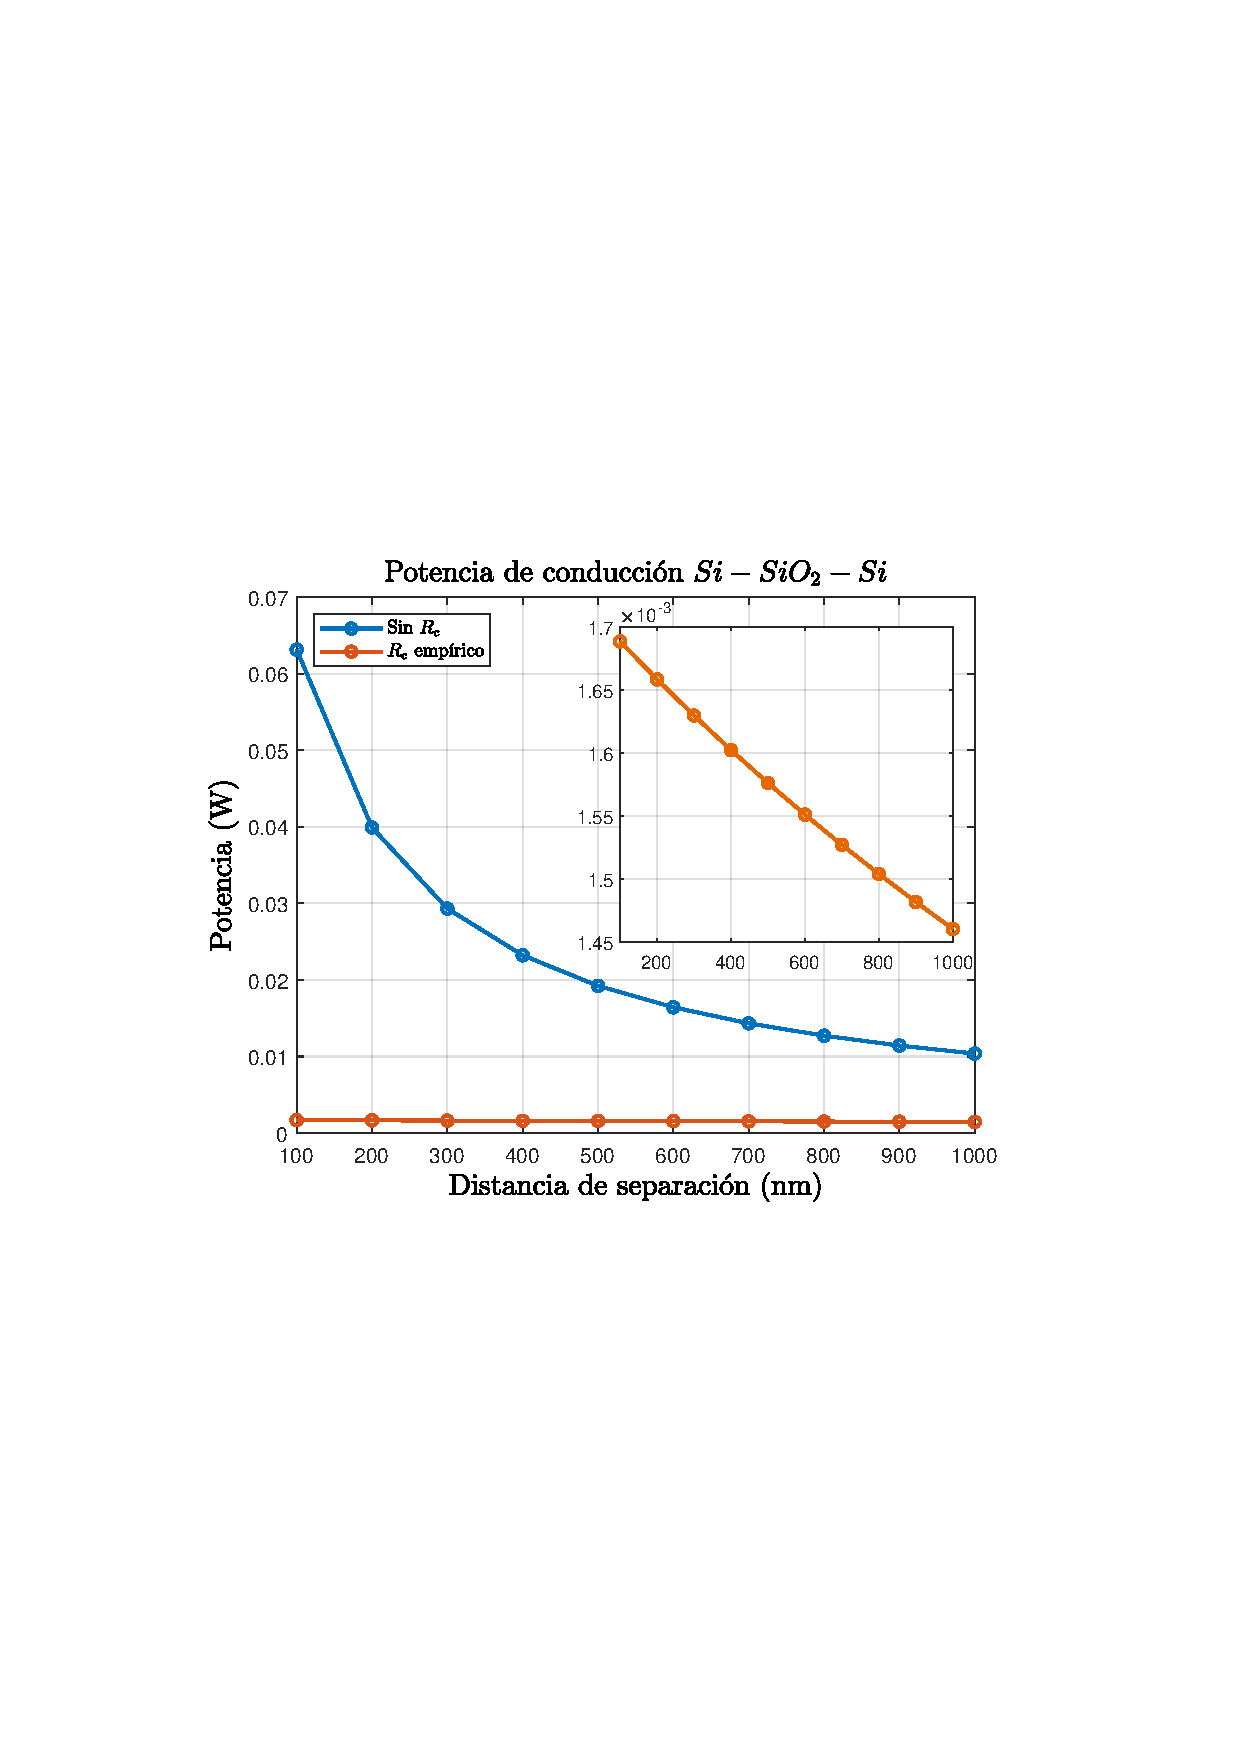
\includegraphics[width=.55\textwidth]{figuras/Resultados/conduccion/pdf/PrcComb2PDF_SiSiO2Si}
	\caption[Efectos de la resistencia de contacto sobre el flujo de calor por conducción]{Representación gráfica del flujo de calor por conducción frente a las diferentes alturas del nano-espaciador con y sin $R_c$. Comparación de la potencia conducida de un nano-espaciador sin $R_c$ y con $R_c$ sobre un mismo eje. Y en el recuadro la potencia conducida de un nano-espaciador con $R_c$.}
	\label{fig:PcondRc_SiSiO2Si}
\end{figure}
Para un área de 9$\mu m^2$ la resistencia de contacto total es aproximadamente de $444.44\cdot 10^3 \ K/W$ comparada con los $85.43\cdot 10^3 \ K/W$ de la mayor resistencia que presenta el nano-espaciador con 1000nm de altura a 25\textdegree C es al menos 5 veces más grande, por lo cual, como se observa en la figura \ref{fig:PcondRc_SiSiO2Si} la resistencia de contacto constante domina sobre la resistencia del nano-espaciador dando así la forma aproximada de una recta (recuadro de la figura \ref{fig:PcondRc_SiSiO2Si}) porque la mayor caída de temperatura se dá en la superficie de contacto, evitando que aumente la temperatura del nano-espaciador variando menos su resistencia térmica (figuras \ref{fig:Pcond_SiSiO2Si_CFD} y \ref{fig:Pcond_SiSiO2Si_Rc_CFD}).
\graphicspath{ {./figuras/Resultados/conduccion/} }
\begin{figure}[H]
	\centering 		% cond sin Rc
	\begin{subfigure}[b]{0.49\textwidth}
	\centering
		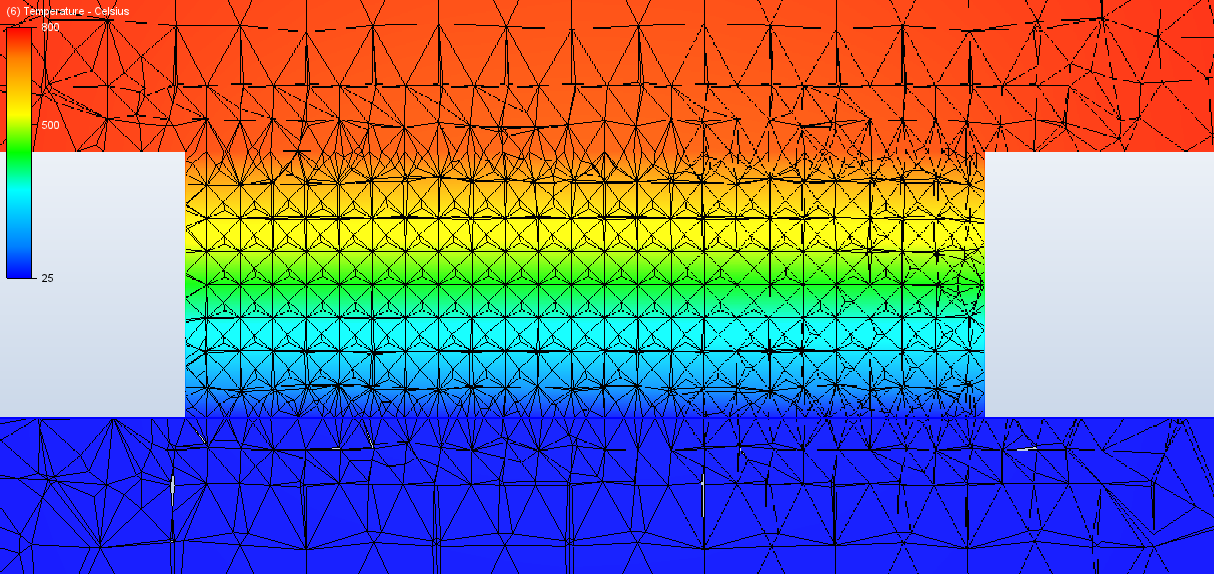
\includegraphics[width=1.00\textwidth]{SiSiO2Si_1000nm_Plane2.png}
		\caption{ }
	\label{fig:Pcond_SiSiO2Si_CFD}
\end{subfigure}
\hfill 					% cond con Rc
\begin{subfigure}[b]{0.49\textwidth}
	\centering
		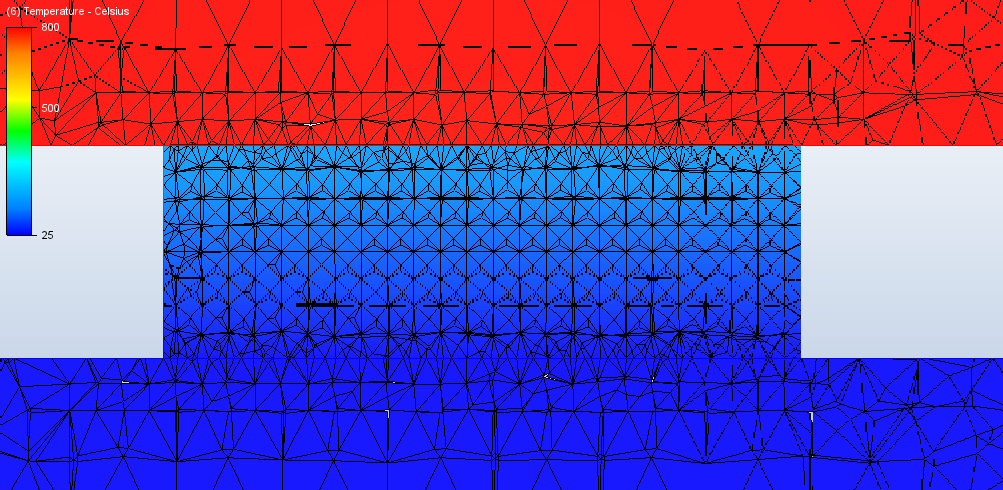
\includegraphics[width=1.00\textwidth]{SiSiO2Si_1000nm_Plane_Rc.png}
		\caption{ }
	\label{fig:Pcond_SiSiO2Si_Rc_CFD}
\end{subfigure}
\caption{Resultados gráficos de la simulación de CFD de la transmisión de calor por conducción a través de un nano-espaciador de 1000nm de altura sin $R_c$ (\subref{fig:Pcond_SiSiO2Si_CFD}) y con $R_c$ (\subref{fig:Pcond_SiSiO2Si_Rc_CFD}).}
	\label{fig:Pconds_SiSiO2Si_CFD}
\end{figure}
La disminución de flujo de calor por conducción es significativa para todos los casos, siendo la potencia de conducción con $R_c$ variando aproximadamente entre un 3\% y un 14\% de la potencia sin $R_c$, lo que implica una disminución de conducción de unos 97\% y 85\%.\\\\
Hay que tomar en cuenta que la resistencia de contacto en la realidad no es constante con la temperatura a diferencia de las simulaciones en CFD donde la $R_c$ es constante, pero sirve para tener una primera idea de su importancia en la eliminación de la transferencia de calor por conducción.
%%%%%%%%%%%%%%%%%%%%%%%%%%%%%%%%%%%%%%%%%%%%%%%%%%%%%%%%
%             POROSIDAD
\subsection{Efecto de la porosidad sobre la conducción}
%% Ahora a comentar sobre las porosidades
Para diferentes porosidades la conductividad térmica varía, disminuyendo con el aumento del grado de porosidad \cite{ThermalConductivity_SiO2_2018}, por este motivo la potencia de conducción disminuye para todas las alturas de nano-espaciador. La relación o conductividad térmica normalizada para una porosidad del 25\% y 50\% son respectivamente 0.64 y 0.25 veces la conductividad térmica del material según la referencia \cite{ThermalConductivity_SiO2_2018}.\\\\
Como se puede observar en la figura \ref{fig:relPpor_SiSiO2Si} las relaciones de potencia no se cumplen completamente porque la temperatura en todo el nano-espaciador no es la misma lo que produce que la conductividad térmica a lo largo del espaciador sea distinta. Por tal motivo, al disminuir la altura del nano-espaciador aumenta la relación porque aumenta el gradiente de temperatura.
\begin{figure}[H]
\centering
	\begin{subfigure}[b]{0.49\textwidth}
		\centering
		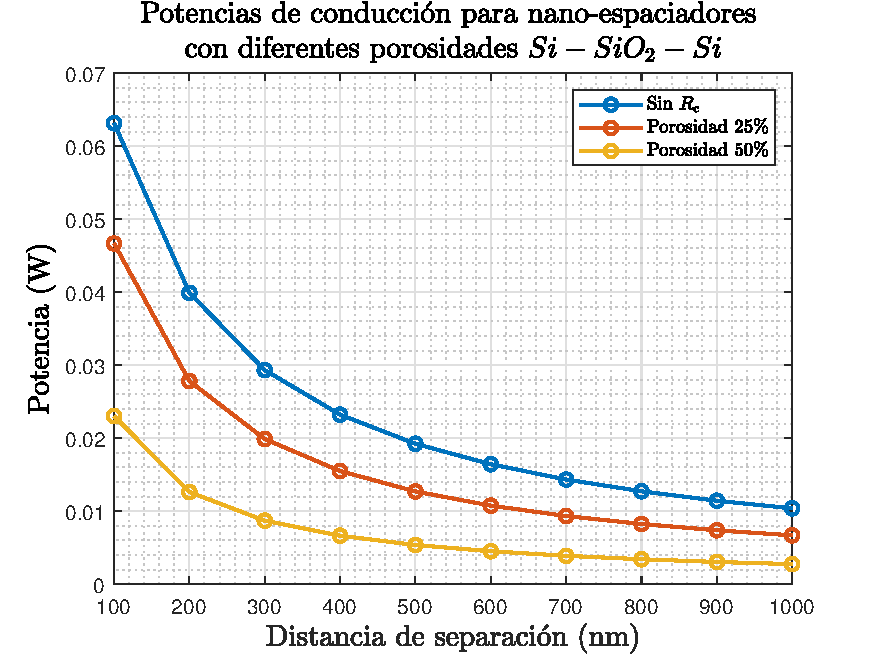
\includegraphics[width=1.0\textwidth]{figuras/Resultados/conduccion/pdf/Ppor_SiSiO2Si.pdf}
		\caption{ }
		\label{fig:Ppor_SiSiO2Si}
	\end{subfigure}
	\hfill
	\begin{subfigure}[b]{0.49\textwidth}
		\centering
		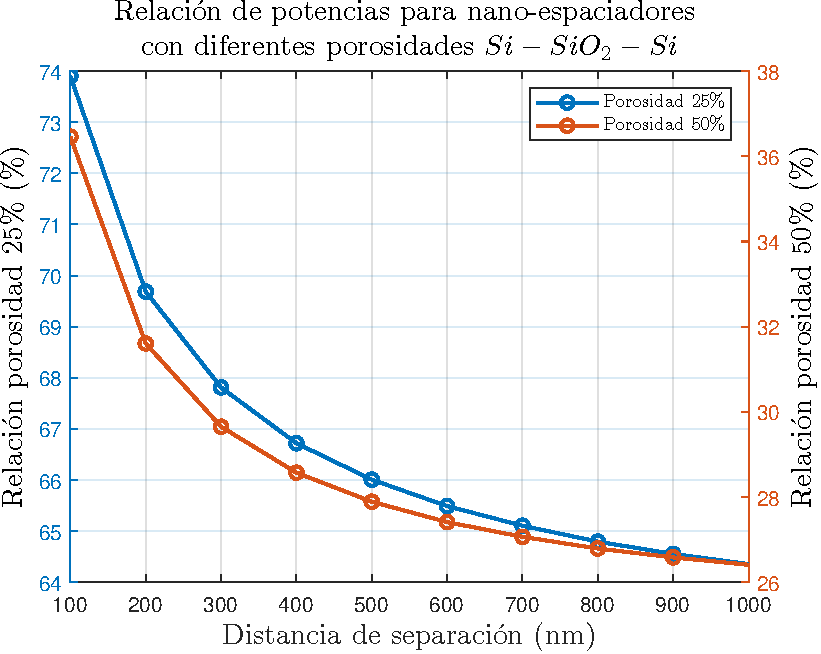
\includegraphics[width=1.0\textwidth]{figuras/Resultados/conduccion/pdf/relPpor_SiSiO2Si.pdf}
		\caption{ }
		\label{fig:relPpor_SiSiO2Si}
	\end{subfigure}
	\caption[Efectos de la porosidad del nano-espaciador sobre el flujo de calor por conducción]{(\subref{fig:Ppor_SiSiO2Si}) Representación gráfica de las potencias de calor transmitidas por conducción  a través de un nano-espaciador frente a la variación de la altura del nano-espaciador para diferentes grados de porosidad del 0\%, 25\% y 50\% del $SiO_2$ y su modelo analítico (ec. \eqref{eq:Pcond_d_p}). (\subref{fig:relPpor_SiSiO2Si}) Representación gráfica de las relaciones de las potencias por conducción para porosidades del $SiO_2$ de 25\% y 50\% respecto a la potencia de 0\% de porosidad frente a la variación de la altura del nano-espaciador.}
	\label{fig:PcondPor_SiSiO2Si}
\end{figure}
Utilizando la aplicación \textbf{Curve Fitting} de MATLAB se obtiene un modelo matemático que relaciona la potencia de conducción respecto a la altura del nano-espaciador ($d$) y la porosidad del material del nano-espaciador ($\rho$), como se muestra en la ecuación \eqref{eq:Pcond_d_p} donde $d$ es en nanómetros.
\begin{equation}
P(d,\rho)=- \frac{  16.47\cdot \rho-11.03 }{d-106.80\cdot \rho +74.68}
\label{eq:Pcond_d_p}
\end{equation}\vspace{2cm}
%%%%%%%%%%%%%%%%%%%%%
%% RAD Si-SiO2-Si
\subsection{Radiación de campo cercano}
Para la radiación por campo cercano se utiliza la aplicación descrita en la sección \ref{sec:calc_campo_cercano} para dos placas gruesas de $Si$ para varias separaciones entre ellas. La potencia radiativa (figura \ref{fig:rad_SiSi_ds}) aumenta con la disminución de la distancia de separación como lo indica el componente exponencial en la ecuación \eqref{eq:flujoEvasNF} de \cite{nfTPV_equations}.
\begin{figure}[H]
	\centering
		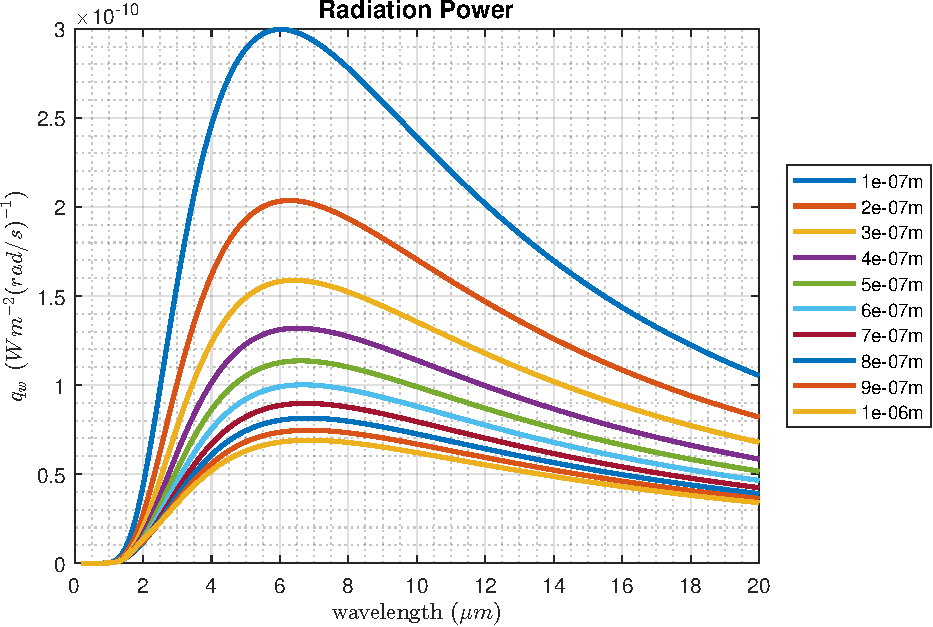
\includegraphics[width=0.65\textwidth]{figuras/Resultados/radiacion/SiSi_ds.pdf}
	\caption{Potencia radiada espectral ($q_w$) para dos placas gruesas planas de $Si$ en todo el rango espectral frente a diferentes distancias de separación de las placas ($d$) en metros.\sourceSpectralRadiation}
	\label{fig:rad_SiSi_ds}
\end{figure}
Integrando la potencia en el rango espectral de longitudes de onda con energías mayores a 1.1 eV, BG del $Si$, se obtiene en promedio potencias del orden de $60 \ W/m^2$ (figura \ref{fig:prad_Eg11_SiSi}) a diferencia de integrar en todo el rango espectral, hasta las $\sim$20 $\mu m$, cuyo orden es de $10^4 \ W/m^2$ (figura \ref{fig:prad_full_SiSi}), Lo cual indica que se desaprovecha una gran cantidad de energía.
\begin{figure}[H]
	\centering
		\begin{subfigure}[b]{0.49\textwidth}
	\centering
		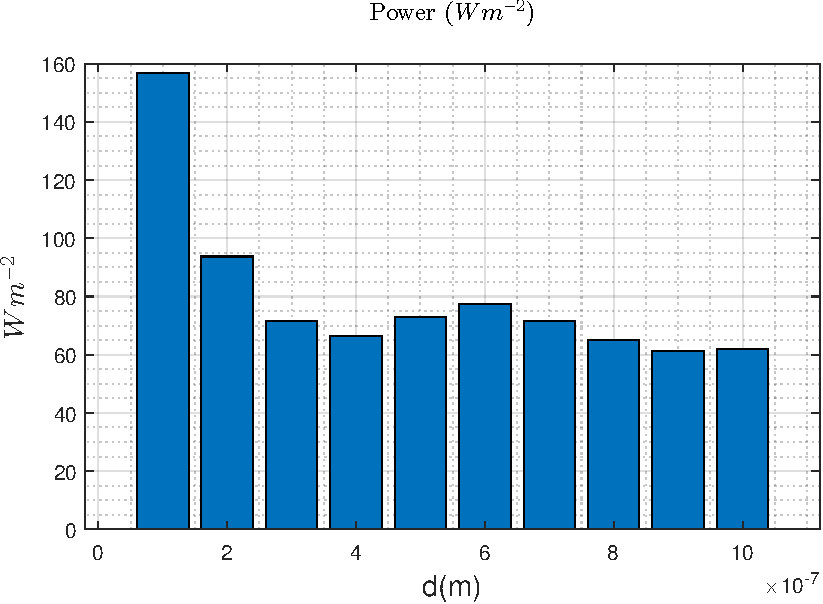
\includegraphics[width=1.00\textwidth]{figuras/Resultados/radiacion/p_11_SiSi.pdf}
	\caption{ }
	\label{fig:prad_Eg11_SiSi}
\end{subfigure}
\hfill
\begin{subfigure}[b]{0.49\textwidth}
	\centering
		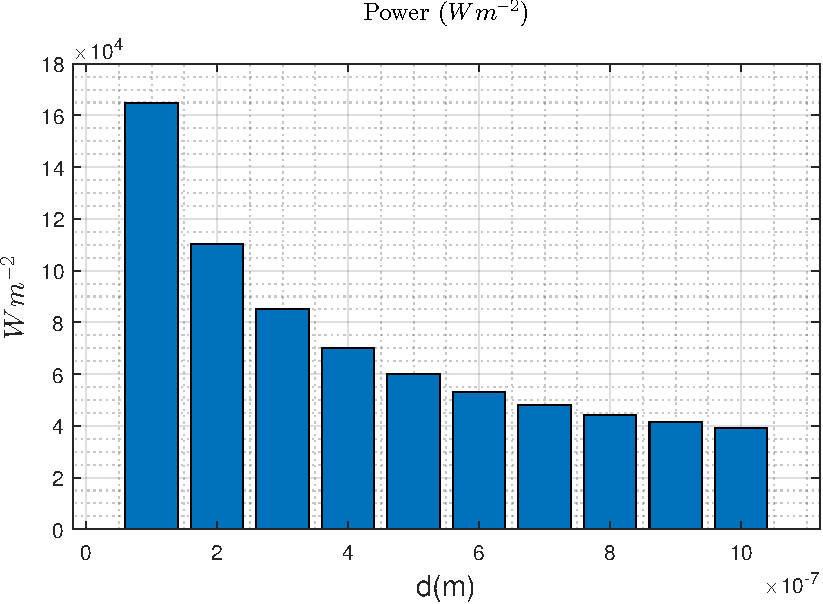
\includegraphics[width=1.00\textwidth]{figuras/Resultados/radiacion/p_full_SiSi.pdf}
	\caption{ }
	\label{fig:prad_full_SiSi}
\end{subfigure}
	\caption{Potencias por unidad de área transmitida por radiación por efecto de campo cercano para el rango espectral de energía mayor a 1.1 eV (\subref{fig:prad_Eg11_SiSi}) y para todo el rango espectral (\subref{fig:prad_full_SiSi}) frente a las diferentes distancias de separación.}
	\label{fig:prad_SiSi}
\end{figure}
Las potencias radiadas frente a las alturas de los nano-espaciadores obtenidas para el rango de longitudes de onda mayor a la BG del $Si$ son muy pequeñas, como se observa en la figura \ref{fig:prad_Eg11_SiSi}, produciendo que no sea viable este sistema porque las pérdidas por conducción son demasiado grandes. Esto se puede visualizar en la figura \ref{fig:rel_SiSi11_Rc}, donde ni siquiera asumiendo la presencia de un único nano-espaciador con Rc se consigue que la potencia radiada sea al menos un orden de magnitud más alta que la potencia transferida por conducción (no se alcanza un factor 10).
\begin{figure}[H]
	\centering
\begin{subfigure}[b]{0.49\textwidth}
	\centering
		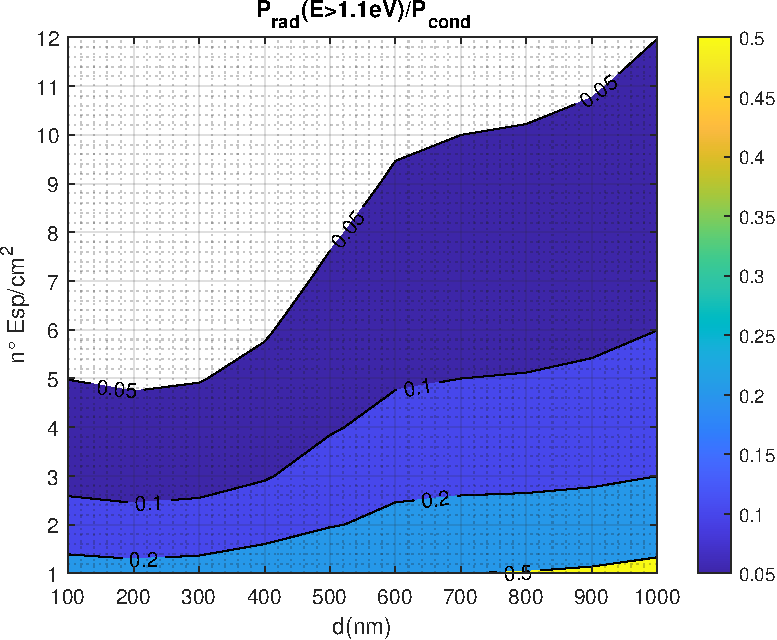
\includegraphics[width=1.00\textwidth]{figuras/Resultados/RelacionCondRad/rel_SiSi11.pdf}
	\caption{ }
	\label{fig:rel_SiSi11}
\end{subfigure}
\hfill
\begin{subfigure}[b]{0.49\textwidth}
	\centering
		\includegraphics[width=1.00\textwidth]{figuras/Resultados/RelacionCondRad/rel_SiSi11_Rc.pdf}
	\caption{ }
	\label{fig:rel_SiSi11_Rc}
\end{subfigure}
\caption{\small  Relación entre la potencia radiada para energías mayores e igual a 1.1 eV y la potencia transmitida por conducción para distintas densidades de nano-espaciadores (eje y) y distintas alturas de los mismos (eje x), con (\subref{fig:rel_SiSi11_Rc}) y sin (\subref{fig:rel_SiSi11}) $R_c$ térmica para una célula de 1 $cm^2$ de $Si$ y emisor de $Si$. La barra de colores lateral representa los colores asociados a cada uno de los valores de las relaciones de potencias, con los contornos de las relaciones más significativas representadas en las gráficas.
%Densidad de los nano-espaciadores para diferentes relaciones de las potencias de radiación en el rango espectral de energía mayor a 1.1 eV respecto a las de conducción para cada densidad de nano-espaciadores de un sistema nTPV de 1$cm^2$ y célula de $Si$ sin $R_c$ (\subref{fig:rel_SiSi11}) y con $R_c$ (\subref{fig:rel_SiSi11_Rc}) frente a las diferentes alturas de los nano-espaciadores. La barra de colores al lateral de cada gráfica representa todas las relaciones entre ambas potencias para diferentes densidades de nano-espaciadores en el rango que se muestra en los extremos de cada barra. También se muestran los contornos con su valor para destacar las distintas relaciones existentes de una manera sencilla.
}
	\label{fig:rels_SiSi11}
\end{figure}
%% RELACION ENTRE COND Y RAD
Para tener una primera mejor idea de los valores numéricos de los resultados obtenidos de las simulaciones de transmisión de calor por conducción y radiación de campo cercano se recopilan en la tabla \ref{tab:condTerSiSiO2Si}, estando en notación científica y con los decimales necesarios para una clara diferenciación de los resultados con el cambio de la distancia de separación entre emisor y célula.
\begin{table}[H]
	\centering
		\caption[Tabla de resultados de las simulaciones de conducción y radiación de campo cercano para diferentes alturas del nano-espaciador. Flujos de calor del nTPV $Si-SiO_2-Si$ para diferentes alturas del nano-espaciador, para los casos sin $R_c$ y con $R_c$ igual a $4 \cdot 10^{-6} \ m^2 K/W$, y sin $R_c$ pero con las proporciones de las porosidades de unos 25\% y un 50\%.]{Tabla de resultados de las simulaciones de conducción y radiación de campo cercano para diferentes alturas del nano-espaciador. Flujos de calor del nTPV $Si-SiO_2-Si$ para diferentes alturas del nano-espaciador, para los casos sin $R_c$ y con $R_c$ igual a $4 \cdot 10^{-6} \ m^2 K/W$ \cite{nf_TPV_Pillars_SiO2}, y sin $R_c$ pero con las proporciones de las porosidades de \cite{ThermalConductivity_SiO2_2018} para un 25\% y un 50\%.}	
		\begin{tabular}{|c||c|c|c|c||c|c|}
		\hline
			\multirow{2}{*}{ }& \multicolumn{6}{c|}{\textbf{\large Potencias según como se transmite el calor}}\\ \cline{2-7}
		  & \multicolumn{4}{c||}{Conducción (W/nº nano-espaciadores)}& \multicolumn{2}{c|}{Radiación $(W/m^2)$}\\ \hline
			Dist. (nm)&$P_{Normal}$&$P_{R_c-Empirico}$&$P_{Porosidad25}$&$P_{Porosidad50}$&$P_{Eg>1.1eV}$&$P_{full}$\\ \hline \hline
			100&6,31E-02&1,69E-03&4,67E-02&2,30E-02&156.89&1,65E+05\\ \hline
			200&3,99E-02&1,66E-03&2,78E-02&1,26E-02&93.75&1,10E+05\\ \hline
			300&2,93E-02&1,63E-03&1,99E-02&8,69E-03&71.75&8,51E+04\\ \hline
			400&2,32E-02&1,60E-03&1,55E-02&6,63E-03&66.39&7,01E+04\\ \hline
			500&1,92E-02&1,58E-03&1,27E-02&5,36E-03&73.00&6,02E+04\\ \hline
			600&1,64E-02&1,55E-03&1,08E-02&4,50E-03&77.52&5,32E+04\\ \hline
			700&1,43E-02&1,53E-03&9,33E-03&3,88E-03&71.63&4,80E+04\\ \hline
			800&1,27E-02&1,50E-03&8,24E-03&3,41E-03&64.90&4,43E+04\\ \hline
			900&1,14E-02&1,48E-03&7,38E-03&3,04E-03&61.42&4,14E+04\\ \hline
		 1000&1,04E-02&1,46E-03&6,68E-03&2,74E-03&62.09&3,93E+04\\ \hline
		\end{tabular}
	\label{tab:condTerSiSiO2Si}
\end{table}
Cabe destacar que la potencia de conducción depende del número de nano-espaciadores y la potencia de radiación depende del área. Por lo tanto, para compararlas hay que multiplicar el número de nano-espaciadores por la potenia de conducción y el área en metros cuadrados a la potencia de radiación integrada.
\vfill \newpage
%%% AHORA EL CASO DE Si SiO2 y Ge
\section{Resultados de las simulaciones para una nTPV de Si-SiO2-Ge}\label{sec:res_SiSiO2Ge}
A continuación se procede a estudiar un caso más realista del sistema nTPV descrito en la sección anterior con una célula de $Ge$ en vez de una de $Si$, cuya BG es de 0.7 eV respecto a los 1.1 eV del $Si$.
\subsection{Simulaciones de CFD}
Se realizan las simulaciones de transmisión de calor por conducción en CFD, obteniéndose una reducción considerable de la potencia de la nTPV con $R_c$ (figura \ref{fig:Prc_SiSiO2Ge}) respecto a sin $R_c$ (figura \ref{fig:Pn_SiSiO2Ge}), como en el caso de la célula de $Si$ (figura \ref{fig:PcondRc_SiSiO2Si}).
\graphicspath{ {./figuras/Resultados/conduccion/pdf/} }
\begin{figure}[H]
	\centering
	%% Si-SiO2-Si Eg
	\begin{subfigure}[b]{0.49\textwidth}
		\centering
		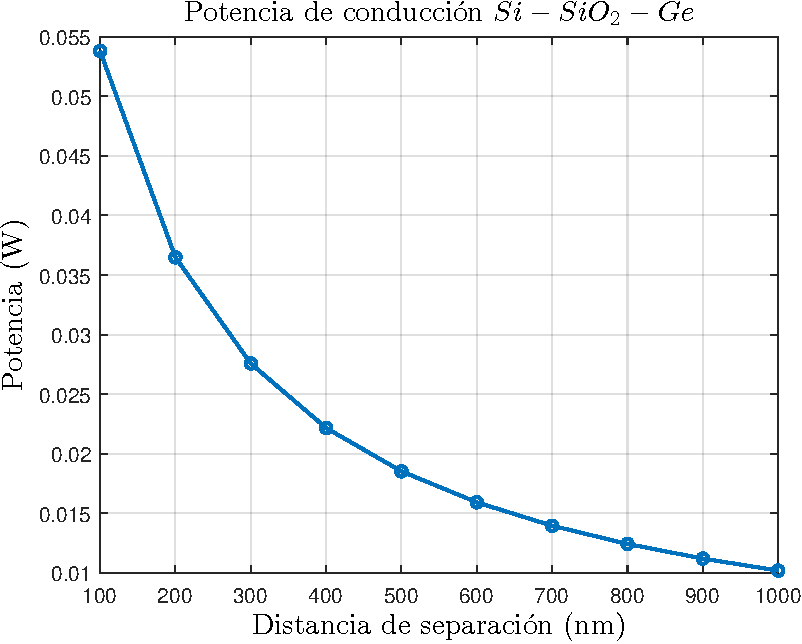
\includegraphics[width=1\textwidth]{Pn_SiSiO2Ge.pdf}
		\caption{ }
		\label{fig:Pn_SiSiO2Ge}
	\end{subfigure}
	\hfill
	\begin{subfigure}[b]{0.49\textwidth}
		\centering
		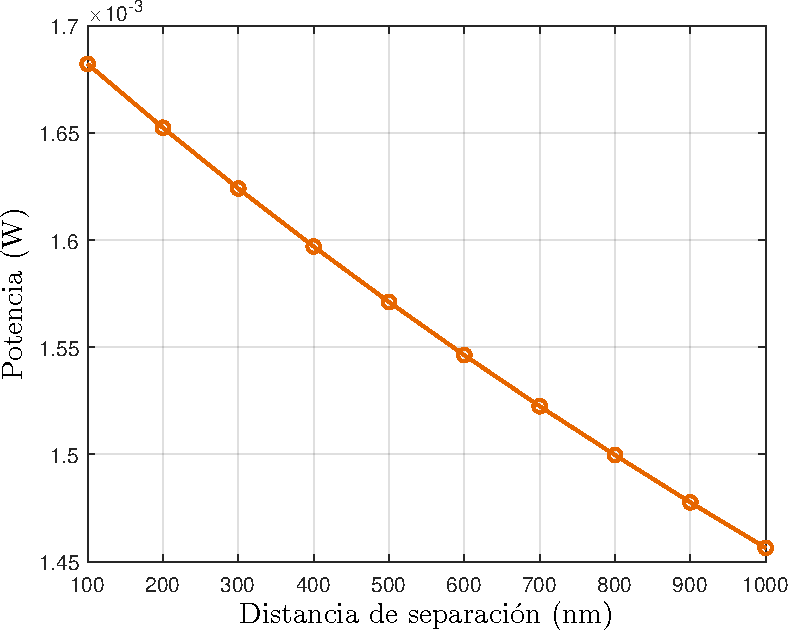
\includegraphics[width=1.00\textwidth]{Prc2_SiSiO2Ge.pdf}
		\caption{ }
		\label{fig:Prc_SiSiO2Ge}
	\end{subfigure}
	\caption{Potencias transmitidas por conducción para un sistema nTPV de $Si-SiO_2-Ge$ de un nano-espaciador con emisor a 800\textdegree C y célula a 25\textdegree C sin $R_c$ (\subref{fig:Pn_SiSiO2Ge}) y con $R_c$ (\subref{fig:Prc_SiSiO2Ge}) frente a las diferentes alturas de nano-espaciador.}
	\label{fig:Pcond_SiSiO2Ge}
\end{figure}
La potencia de conducción disminuye de unos 53.80 $mW$ sin $R_c$ a unos 1.68 $mW$ con $R_c$ para una altura de nano-espaciador de 100nm, que representa una reducción del 96.87\%. Para unos 1000 nm de altura de nano-espaciador la potencia disminuye de unos 10.20 $mW$ sin $R_c$ a unos 1.46 $mW$ con $R_c$, que representa una reducción del 85.69 \%.\\\\
Comparando los resultados obtenidos de la simulación de transmisión de calor por conducción de la nTPV de célula de $Ge$ respecto a la de $Si$, se observa una variación casi nula para cuando hay $R_c$. Siendo aproximadamente las potencias de conducción de la nTPV con célula de $Ge$ un 99\% de las potencias de la nTPV con célula de $Si$ para todas las alturas del nano-espaciador, dando a entender que la diferencia de la conductividad térmica de los materiales no produce un efecto significativo sobre la conducción cuando existe $R_c$. Para el caso de que la nTPV no tenga $R_c$, las potencias para la célula de $Ge$ son entre un $\sim$85\% y un $\sim$98\% respecto a la de la célula de $Si$.
\vfill
\subsection{Radiación de campo cercano}
De las simulaciones de radiación de campo cercano se obtienen también resultados muy parecidos a los obtenidos en el caso de la célula de $Si$ (figura \ref{fig:SiSi_vs_SiGe}), solo mostrándose hasta los $\sim$14$\mu m$ de longitud de onda, donde se observa como al disminuir la distancia de separación aumenta la potencia radiativa (figura \ref{fig:rad_SiGe}).
\begin{figure}[H]
\centering
\begin{subfigure}[b]{0.49\textwidth}
	\centering
		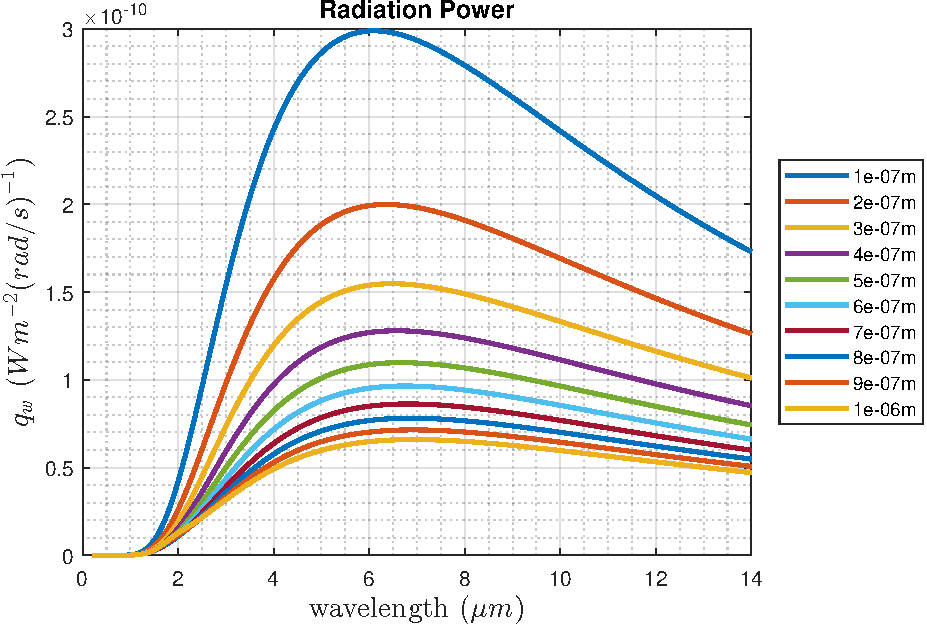
\includegraphics[width=1.00\textwidth]{figuras/Resultados/radiacion/SiGe.pdf}
	\caption{ }
	\label{fig:rad_SiGe}
\end{subfigure}
\hfill
\begin{subfigure}[b]{0.49\textwidth}
	\centering
		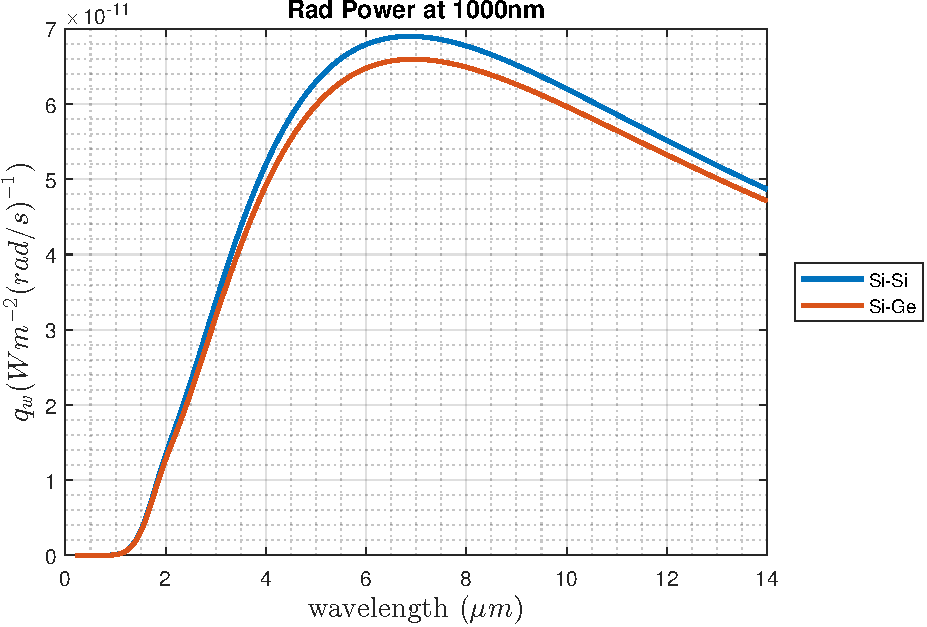
\includegraphics[width=1.00\textwidth]{figuras/Resultados/radiacion/SiSi_vs_SiGe.pdf}
	\caption{ }
	\label{fig:SiSi_vs_SiGe}
\end{subfigure}
\caption{Potencia radiada espectral ($q_w$) por campo cercano para un sistema nTPV $Si-SiO_2-Ge$ frente a las longitudes de onda para varias distancias de separación entre placas(\subref{fig:rad_SiGe}) y para dos materiales de célula, $Si$ y $Ge$ (\subref{fig:SiSi_vs_SiGe}).}
\label{fig:rads_SiGe}
\end{figure}
Para la obtención de las potencias de radiación se procede a realizar la integral en el rango espectral de energía mayor a los 0.7 eV, obteniéndose potencias alrededor de los $10^3 \ W/m^2$ (figura \ref{fig:p_Eg_SiGe}), y para todo el rango espectral de longitudes de onda se obtiene potencias alrededor de los $10^4 \ W/m^2$ con un máximo de $\sim$1.5$10^5 \ W/m^2$ (figura \ref{fig:p_full_SiGe} y tabla \ref{tab:SiSiO2Ge}). 
%% POTENCIAS INTEGRADAS
\begin{figure}[H]
\centering
\begin{subfigure}[b]{0.49\textwidth}
	\centering
		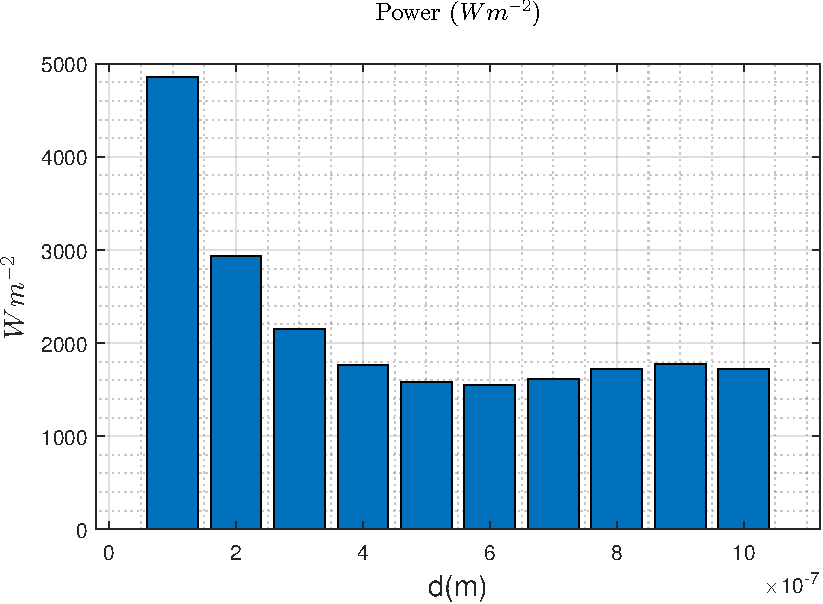
\includegraphics[width=1.00\textwidth]{figuras/Resultados/radiacion/p_Eg_SiGe.pdf}
	\caption{P }
	\label{fig:p_Eg_SiGe}
\end{subfigure}
\hfill
\begin{subfigure}[b]{0.49\textwidth}
	\centering
		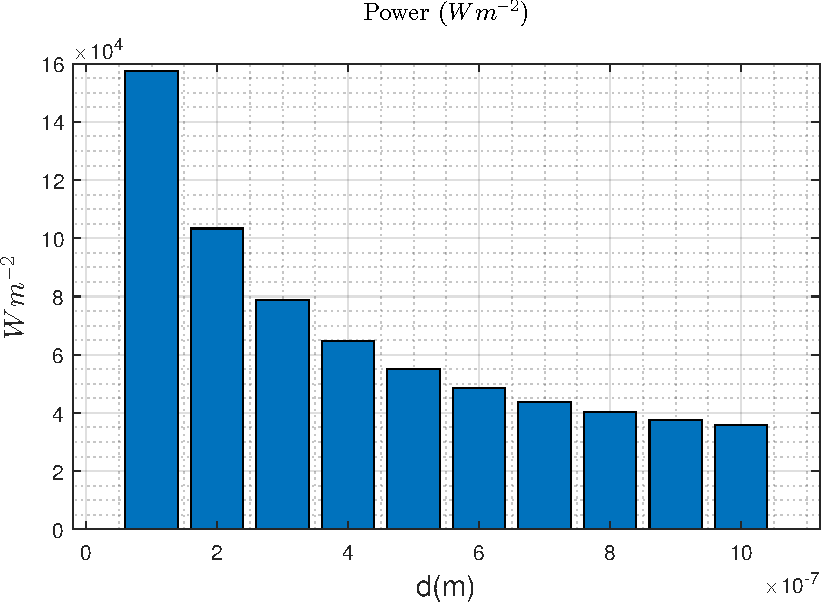
\includegraphics[width=1.00\textwidth]{figuras/Resultados/radiacion/p_full_SiGe.pdf}
	\caption{ }
	\label{fig:p_full_SiGe}
\end{subfigure}
	\caption[Potencias por unidad de área para la radiación de campo cercano para el sistema $Si-SiO_2-Ge$ frente a las diferentes alturas del nano-espaciador]{Potencias por unidad de área para la radiación de campo cercano para el sistema $Si-SiO_2-Ge$ frente a las diferentes alturas del nano-espaciador. (\subref{fig:p_Eg_SiGe}) Potencias en el rango espectral de todas las longitudes de onda de energía mayor a 0.7 eV. (\subref{fig:p_full_SiGe}) Potencias en todo el rango espectral, hasta las $\sim$14$\mu m$.}
	\label{fig:p_SiGe}
\end{figure}
Como para el caso de la nTPV de $Si-SiO_2-Si$ la diferencia de la potencia entre integrar hasta los 0.7 eV del rango espectral e integrar en todo el rango espectral es significativa. Al cambiar la célula de $Si$ por una de menor BG de $Ge$ se aumenta la cantidad de potencia que se puede convertir en electricidad. También se observa una disminución de las potencias alrededor de los 600 nm (figura \ref{fig:p_Eg_SiGe}), a diferencia de la célula de $Si$ que aumenta debido al efecto Fabry-Perot (\ref{fig:prad_Eg11_SiSi}).
%%%   DENSIDAD DE NANO-ESPACIADORES
\subsection{Densidad de nano-espaciadores}
Para tener una mejor percepción de las ventajas que presenta el usar una célula de $Ge$ frente a una de $Si$ se calcula la densidad de nano-espaciadores frente a las alturas del nano-espaciador para las relaciones de la potencia de radiación respecto a la de conducción, observando que para las mismas alturas de nano-espaciador y densidades similares, se obtienen valores mucho mayores.\\\\
Hay que tener en cuenta que para un centímetro cuadrado de superficie de radiación la transmisión de calor por radiación se ve multiplicado por $10^{-4}$, por lo tanto, la potencia de radiación con $E_g>0.7eV$ en un centímetro cuadrado es $\sim$10 veces mayor que la potencia conducida sin resistencia de contacto para un nano-espaciador (figura \ref{fig:rel_SiSiO2Ge}), pero $\sim$100 veces mayor que la potencia conducida con resistencia de contacto (figura \ref{fig:rel_SiSiO2Ge_Rc}).
\begin{figure}[H]
	\centering
	%% Si-SiO2-Si Eg
	\begin{subfigure}[b]{0.49\textwidth}
		\centering
		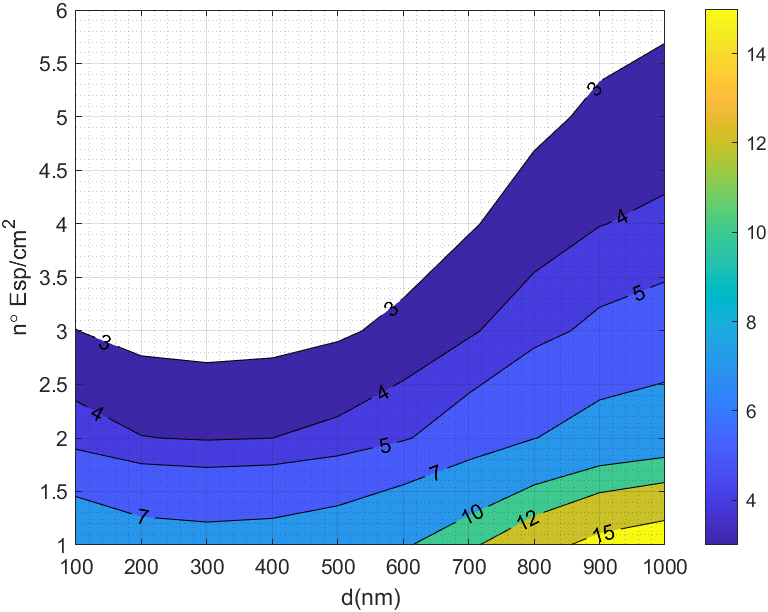
\includegraphics[width=1.00\textwidth]{figuras/Resultados/RelacionCondRad/SiGe.png}
		\caption{ }
		\label{fig:rel_SiSiO2Ge}
	\end{subfigure}
	\hfill
	\begin{subfigure}[b]{0.49\textwidth}
			\centering
			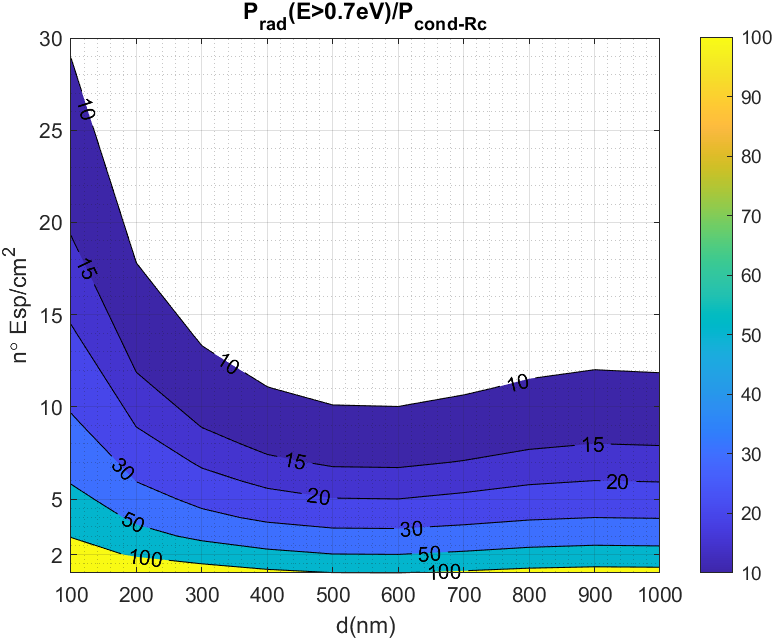
\includegraphics[width=1.00\textwidth]{figuras/Resultados/RelacionCondRad/SiGe_Rc.png}
			\caption{ }
			\label{fig:rel_SiSiO2Ge_Rc}
		\end{subfigure}
	\caption{\small Relación entre la potencia radiada para energías mayores e igual a 0.7 eV y la potencia transmitida por conducción para distintas densidades de nano-espaciadores (eje y) y distintas alturas de los mismos (eje x), con (\subref{fig:rel_SiSiO2Ge_Rc}) y sin (\subref{fig:rel_SiSiO2Ge}) $R_c$ térmica para una célula de 1 $cm^2$ de $Ge$ y emisor de $Si$. La barra de colores lateral representa los colores asociados a cada uno de los valores de las relaciones de potencias, con los contornos de las relaciones más significativas representadas en las gráficas.
	%Densidad de los nano-espaciadores para diferentes relaciones de las potencias de radiación en el rango espectral de energía mayor a 0.7 eV respecto a las de conducción para cada densidad de nano-espaciadores de un sistema nTPV de 1$cm^2$ y célula de $Ge$ sin $R_c$ (\subref{fig:rel_SiSiO2Ge}) y con $R_c$ (\subref{fig:rel_SiSiO2Ge_Rc}) frente a las diferentes alturas de los nano-espaciadores. La barra de colores al lateral de cada gráfica representa todas las relaciones entre ambas potencias para diferentes densidades de nano-espaciadores en el rango que se muestra en los extremos de cada barra. También se muestran los contornos con su valor para destacar las distintas relaciones existentes de una manera sencilla.
	}
	\label{fig:relation_SiSiO2Ge}
\end{figure}
Como se observa en las figuras \ref{fig:relation_SiSiO2Ge} \subref{fig:rel_SiSiO2Ge} y \subref{fig:rel_SiSiO2Ge_Rc}, la forma de la curva cambia su tendencia según se incluya o no la $R_c$ porque sin $R_c$ la tendencia de la curva de crecer con el aumento de la altura de los nano-espaciadores está marcada por la potencia de conducción (inversamente proporcional), y para el caso con $R_c$ la  tendencia de la curva de aumentar con la disminución de la altura de los nano-espaciadores está marcada por la potencia de radiación de campo cercano.\\\\
Los valores de las relaciones de la potencia de útil respecto a la pérdidas, es decir, la potencia de radiación divido por la potencia de conducción, son bajos para todas las densidades de nano-espaciadores del caso de la nTPV sin $R_c$, apenás consiguiendo una relación de al menos un orden de magnitud solo para una densidad de un 1 nº$esp/cm^2$ con altura mínima de 600 nm, como se puede observar en la figura \ref{fig:rel_SiSiO2Ge}. Para el caso con $R_c$ se consigue como mínimo una relación de dos ordenes de magnitud para todas las alturas de un nano-espaciador, como se puede observar en la figura \ref{fig:rel_SiSiO2Ge_Rc}.\\\\
Estas relaciones disminuyen con el aumento de la densidad de los nano-espaciadores porque aumenta la potencia de conducción, por este motivo solo serán viables aquellas configuraciones que como mínimo tengan una relación de potencias de un orden de magnitud y una configuración mínima de cuatro nano-espaciadores, brindando apoyo y una mayor estabilidad que para un mínimo de tres nano-espaciadores.\\\\
La densidad de nano-espaciadores para una relación de potencias de un orden de magnitud es como mínimo 7 veces mayor para una nTPV con $R_c$ (\ref{fig:rel_SiSiO2Ge_Rc}) respecto a sin $R_c$ (\ref{fig:rel_SiSiO2Ge}), que para dicha relación de potencias su densidad de nano-espaciadores es menor a 4 nº$esp/cm^2$. Para la nTPV con $R_c$, la densidad de nano-espaciadores es mayor que 4 para un relación de potencias de 10.\\\\
Por lo tanto, entre ambos casos el que puede ser viable es el sistema nTPV con $R_c$ porque presenta una mayor densidad de nano-espaciadores para una misma relación de potencias, lo que permite que se distribuya la carga sobre los nano-espaciadores y sea más fácil mantener la separación entre el emisor y la célula constante sobre toda la superficie.
\begin{figure}[H]
		\begin{subfigure}[b]{0.49\textwidth}
		\centering
		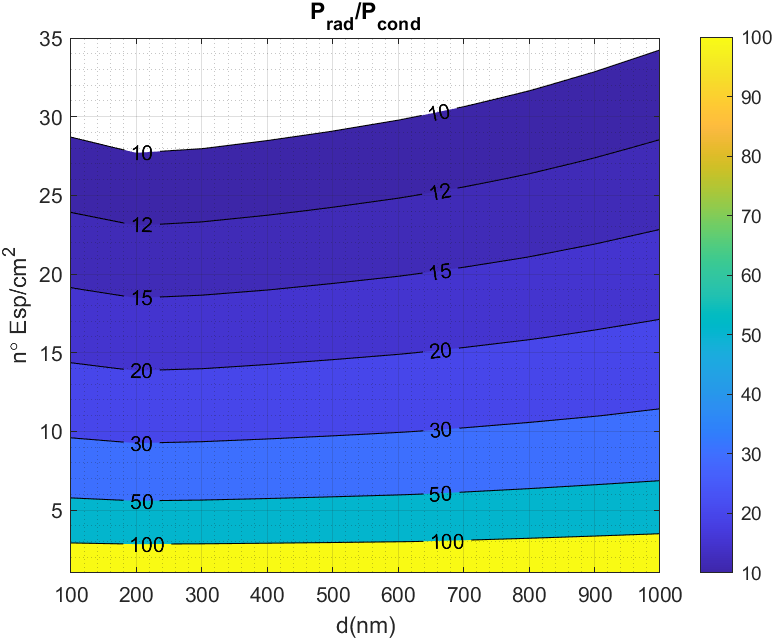
\includegraphics[width=1.00\textwidth]{figuras/Resultados/RelacionCondRad/SiGe_full.png}
		\caption{ }
		\label{fig:rel_SiSiO2Ge_full}
	\end{subfigure}
		\hfill
		\begin{subfigure}[b]{0.49\textwidth}
			\centering
			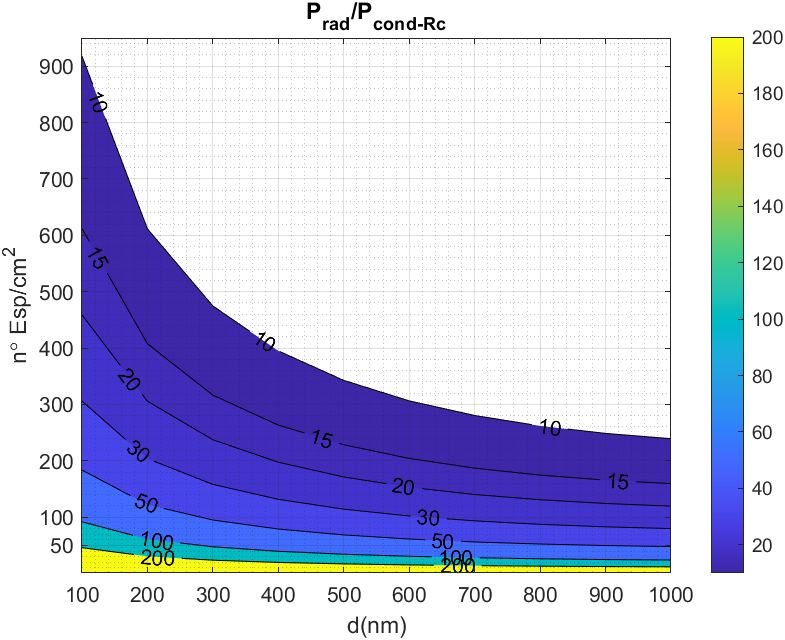
\includegraphics[width=1.00\textwidth]{figuras/Resultados/RelacionCondRad/SiGe_Rc_full_10.png}
			\caption{ }
			\label{fig:rel_SiSiO2Ge_Rc_full}
		\end{subfigure}
	\caption{\small  Relación entre la potencia radiada total y la potencia transmitida por conducción para distintas densidades de nano-espaciadores (eje y) y distintas alturas de los mismos (eje x), con (\subref{fig:SiGe_Rc_full_10}) y sin (\subref{fig:SiGe_full}) $R_c$ térmica para una célula de 1 $cm^2$ de $Ge$ y emisor de $Si$. La barra de colores lateral representa los colores asociados a cada uno de los valores de las relaciones de potencias, con los contornos de las relaciones más significativas representadas en las gráficas.
	%Densidad de los nano-espaciadores para diferentes relaciones de las potencias de radiación en todo el rango espectral respecto a las de conducción para cada densidad de nano-espaciadores de un sistema nTPV de 1$cm^2$ y célula de $Ge$ sin $R_c$ (\subref{fig:rel_SiSiO2Ge_full}) y con $R_c$ (\subref{fig:rel_SiSiO2Ge_Rc_full}) frente a las diferentes alturas de los nano-espaciadores. La barra de colores al lateral de cada gráfica representa todas las relaciones entre ambas potencias para diferentes densidades de nano-espaciadores en el rango que se muestra en los extremos de cada barra. También se muestran los contornos con su valor para destacar las distintas relaciones existentes de una manera sencilla.
	}%
	\label{fig:rels_SiSiO2Ge_full}%
\end{figure}
Por último, se representan el caso de la densidad de nano-espaciadores frente a las alturas de los nano-espaciadores para varias relaciones de las potencias de radiación en todo el rango espectral y las potencias de conducción sin y con $R_c$ (figuras \ref{fig:rels_SiSiO2Ge_full}  \subref{fig:rel_SiSiO2Ge_full} y \subref{fig:rel_SiSiO2Ge_Rc_full}, respectivamente), observándose las mismas tendencias que para el rango espectral de energías mayores e iguales a 0.7 eV pero con mayor densidad de nano-espaciadores por el aumento de la potencia radiada de campo cercano, por lo tanto, el aumento del rango espectral de radiación útil es bastante importante para el aumento de la potencia a convertir en electricidad.\\\\
Para facilitar la revisión de los resultados obtenidos de las simulaciones y de los cálculos realizados se recopilan en la tabla \ref{tab:SiSiO2Ge}, donde se presentan en notación científica para facilitar la observación de los ordenes de magnitud de los resultados.
\begin{table}[H]
	\centering
	\caption{Tabla de las potencias de resultado de las simulaciones de transmisión de calor por radiación de campo cercano y conducción para el sistema nTPV $Si-SiO_2-Ge$.}	
		\begin{tabular}{|c||c|c||c|c|}
		\hline
\multirow{2}{*}{ }& \multicolumn{4}{c|}{\textbf{\large Potencias según transmisión del calor}}\\ \cline{2-5}
& \multicolumn{2}{c||}{Conducción (W/nº esp.)}& \multicolumn{2}{c|}{Radiación $(W/m^2)$}\\ \hline
Dist. (nm)&$P_{Normal}$&$P_{R_c-Empirico}$&$P_{Eg>0.7eV}$&$P_{full}$\\ \hline \hline
100&5,38E-02&1,68E-03&4,87E+03&1,54E+05\\ \hline 
200&3,65E-02&1,65E-03&2,94E+03&1,01E+05\\ \hline 
300&2,76E-02&1,62E-03&2,16E+03&7,71E+04\\ \hline 
400&2,22E-02&1,60E-03&1,77E+03&6,31E+04\\ \hline 
500&1,85E-02&1,57E-03&1,59E+03&5,38E+04\\ \hline 
600&1,59E-02&1,55E-03&1,55E+03&4,74E+04\\ \hline 
700&1,39E-02&1,52E-03&1,62E+03&4,27E+04\\ \hline 
800&1,24E-02&1,50E-03&1,73E+03&3,93E+04\\ \hline 
900&1,12E-02&1,48E-03&1,78E+03&3,67E+04\\ \hline 
1000&1,02E-02&1,46E-03&1,73E+03&3,49E+04\\ \hline 
		\end{tabular}
	\label{tab:SiSiO2Ge}
\end{table}
\vfill
%%% RESULTADOS DE SS
\newpage
%%%%%%%%%%%%%%%%%%%%%%%%%%%%%%%%%%%%%%%%%%%%%%%%%%%%%%%%%%%%%%%%%%%%%%%%%
%               EMISOR DE  STAINLESS STEEL
%%%%%%%%%%%%%%%%%%%%%%%%%%%%%%%%%%%%%%%%%%%%%%%%%%%%%%%%%%%%%%%%%%%%%%%%%
\section{Resultados de las simulaciones para una nTPV de SS-SiO2-Ge}\label{sec:res_SsSiO2Ge}
Una de las razones más importantes del estudio de las nTPV es la recuperación de calor residual, por lo cual se simula la transmisión por conducción y radiación para una nTPV de emisor de acero inoxidable ($SS$) porque es un material altamente utilizado en todos los sectores, principalmente en la industria, ya sea en calderas, tuberías u otros componentes o máquinas se encuentran a altas temperaturas.
%%%%%%%%%%%%%%%%%%%%%%%%%%%%%%%%%%%%
%           CFD
\subsection{Simulaciones de CFD}
Para las simulaciones de transmisión de calor por conducción se estudian los efectos de resistencias de contacto aún mayores a la empírica estudiada hasta ahora. Las nuevas resistencias de contacto se obtienen aplicando la inversa a la \gls{hc} ($R_c=1/h_c$), la cual se obtiene mediante la relación de las $h_c$ según la ecuación \eqref{eq:relacion_conductividadesTermicas} para un emisor de $SS$ y un nano-espaciador liso de $SiO_2$. La $h_c$ utilizada es 1000 $W/(m^2 K)$, que corresponde a la $h_c$ para dos aceros inoxidables a una presión de $\sim$1 GPa para los experimentos realizados en \cite{experimental_Rc_SS}, porque a dicha presión el error respecto al modelo matemático es pequeño.\\\\
A partir de dicha $h_c$ y aplicando la ecuación \eqref{eq:relacion_conductividadesTermicas} se obtiene una $R_c$ de $5.5\cdot 10^{-3} \ m^2 K/W$ para una superficie de SS en contacto con una superficie lisa de $SiO_2$. Se toma un valor intermedio entre dicha $R_c$ y la $R_c$ empírica de $4\cdot 10^{-6} \ m^2 K/W$ \cite{nf_TPV_Pillars_SiO2} para obtener el efecto de la variación de la $R_c$ sobre la transmisión de conducción y la viabilidad del sistema, siendo el valor de dicha $R_c$ intermedia unos $2.75\cdot 10^{-3} \ m^2 K/W$.\\\\
Primero se simula la transmisión de calor por conducción para el caso sin $R_c$ (figura \ref{fig:Pn_SsSiO2Ge}) y con $R_c$ empírica de $4\cdot 10^{-6} \ m^2 K/W$ (figura \ref{fig:Prc_SsSiO2Ge_Emp}), para luego estudiar con $R_c$ calculada de $5.5\cdot 10^{-3} \ m^2 K/W$ (figura \ref{fig:Prc_SsSiO2Ge_Inter}) y con $R_c$ calculada intermedia de $2.75\cdot 10^{-3} \ m^2 K/W$ (figura \ref{fig:Prc_SsSiO2Ge_Max}).
\graphicspath{ {./figuras/Resultados/conduccion/pdf/} }
\begin{figure}[H]
	\centering
	\begin{subfigure}[b]{0.49\textwidth}
		\centering
			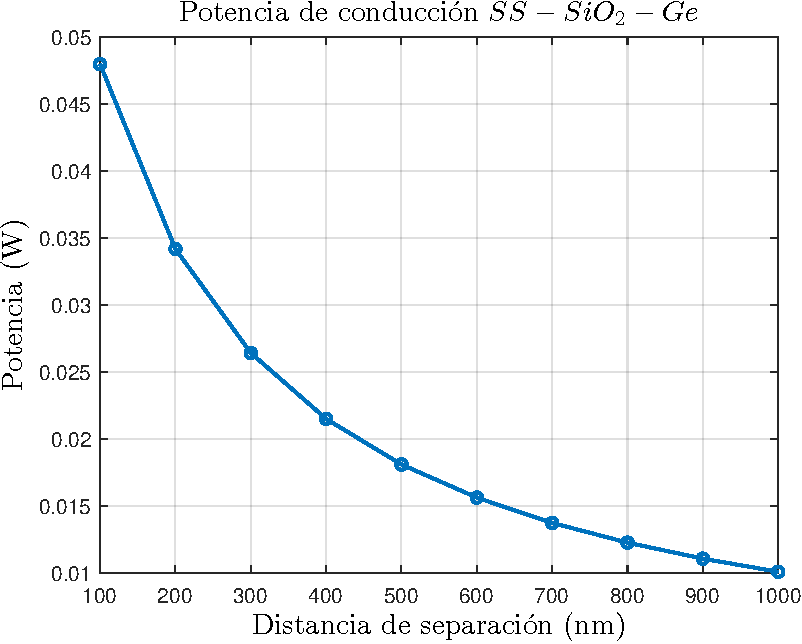
\includegraphics[width=1.00\textwidth]{Pn_SsSiO2Ge.pdf}
		\caption{ }
		\label{fig:Pn_SsSiO2Ge}
	\end{subfigure}
	\hfill
	\begin{subfigure}[b]{0.49\textwidth}
		\centering
			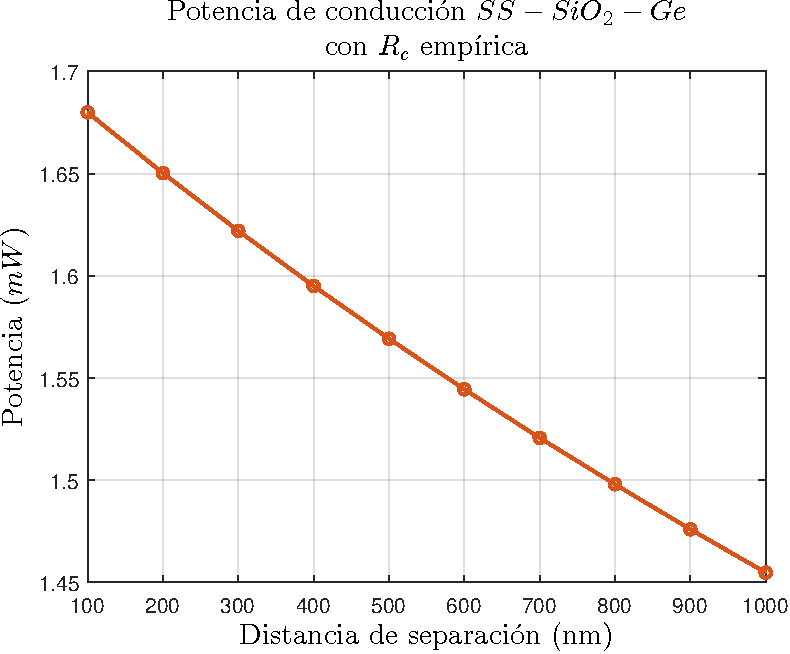
\includegraphics[width=1.00\textwidth]{Prc_SsSiO2Ge_Emp.pdf}
		\caption{ }
		\label{fig:Prc_SsSiO2Ge_Emp}
	\end{subfigure}
	\caption{Potencias transmitidas por conducción para una nTPV $SS-SiO_2-Ge$ sin $R_c$ (\subref{fig:Pn_SsSiO2Ge}) y con $R_c$ empírica de $4\cdot 10^{-6} \ m^2 K/W$ (\subref{fig:Prc_SsSiO2Ge_Emp}) frente a las diferentes alturas de nano-espaciador.}
	\label{fig:Pcond1_SsSiO2Ge}
\end{figure}
La potencia máxima sin $R_c$ es menor que 0.05W (figura \ref{fig:Pn_SsSiO2Ge}) a diferencia de la nTPV de $Si-SiO_2-Ge$ que la potencia máxima es menor a unos 0.055W (figura \ref{fig:Pn_SiSiO2Ge}). Para la nTPV con $R_c$ empírica la potencia conducida se encuentra en el rango de 1.45 $mW$ a 1.7 $mW$ (figura \ref{fig:Prc_SsSiO2Ge_Emp}), igual que para el caso de la nTPV de $Si-SiO_2-Ge$, por lo tanto, el material del emisor no es significativo cuando existe una resistencia de contacto de por lo menos $4\cdot 10^{-6} \ m^2 K/W$.\\\\
Las potencias transmitidas por conducción para los casos con $R_c$ calculadas (figuras \ref{fig:Prc_SsSiO2Ge_Max} \subref{fig:Prc_SsSiO2Ge_Inter} y \subref{fig:Prc_SsSiO2Ge_Max}) son tres ordenes de magnitud menor que para las potencias del caso con $R_c$ empírica (figura \ref{fig:Prc_SsSiO2Ge_Emp}), esta reducción corresponde a que ambas $R_c$ calculadas son tres ordenes de magnitud superior a la $R_c$ empírica. Por ende, la $R_c$ es la resistencia de mayor relevancia del sistema nTPV para cualquiera de estos tres valores.
\begin{figure}[H]
	\centering
	\begin{subfigure}[b]{0.49\textwidth}
		\centering
			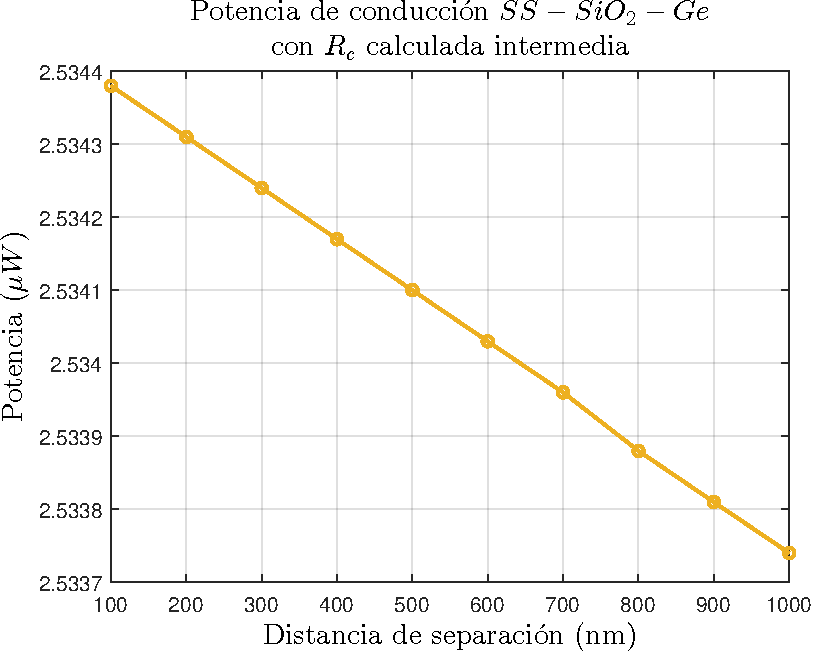
\includegraphics[width=1.00\textwidth]{Prc_SsSiO2Ge_Inter.pdf}
		\caption{ }
		\label{fig:Prc_SsSiO2Ge_Inter}
	\end{subfigure}
	\hfill
	\begin{subfigure}[b]{0.49\textwidth}
		\centering
			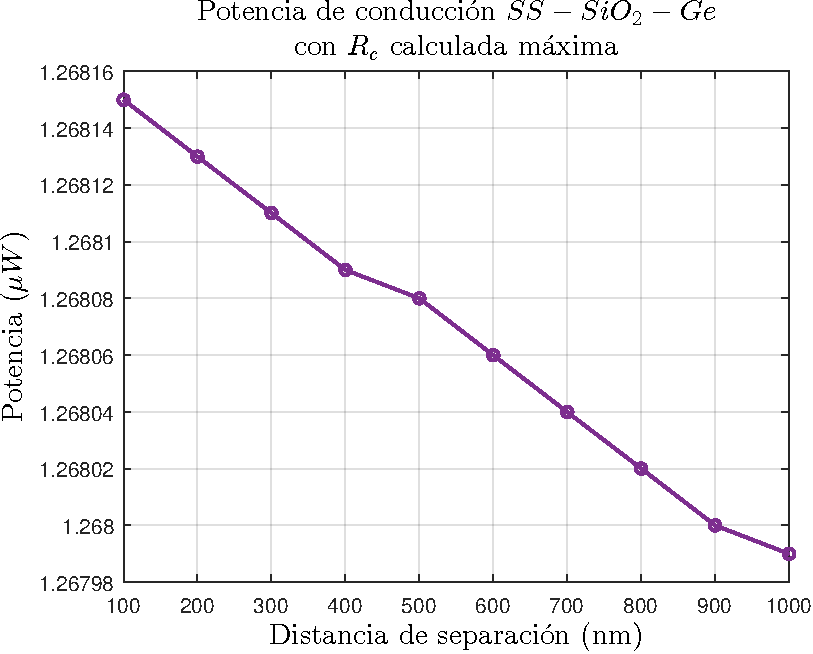
\includegraphics[width=1.00\textwidth]{Prc_SsSiO2Ge_Max.pdf}
		\caption{ }
		\label{fig:Prc_SsSiO2Ge_Max}
	\end{subfigure}
	\caption[Potencias trasmitidas por conducción para una nTPV $SS-SiO_2-Ge$ con $R_c$ calculadas, con una $R_c$ máxima de  $5.5\cdot 10^{-3} \ m^2 K/W$ (\subref{fig:Prc_SsSiO2Ge_Max}) y una $R_c$ intermedia $2.75\cdot 10^{-3} \ m^2 K/W$ (\subref{fig:Prc_SsSiO2Ge_Inter}) frente a las diferentes alturas de un nano-espaciadores.]{Potencias transmitidas por conducción para una nTPV $SS-SiO_2-Ge$ con $R_c$ calculadas a partir de las conductancias térmicas \cite{experimental_Rc_SS}, para una $R_c$ máxima de  $5.5\cdot 10^{-3} \ m^2 K/W$ (\subref{fig:Prc_SsSiO2Ge_Max}) y una $R_c$ intermedia $2.75\cdot 10^{-3} \ m^2 K/W$ (\subref{fig:Prc_SsSiO2Ge_Inter}) frente a las diferentes alturas de nano-espaciador.}
	\label{fig:Pcond2_SsSiO2Ge}
\end{figure}
Las potencias para las nTPV con $R_c$ calculadas son del orden de los mil $n W$, y como se pueden observar en las figuras \ref{fig:Pcond2_SsSiO2Ge} (\subref{fig:Prc_SsSiO2Ge_Inter}) y (\subref{fig:Prc_SsSiO2Ge_Max}) las potencias son aproximadamente rectas con muy poca variación entre cada altura consecutiva de nano-espaciador, pudiéndose considerarse constantes para unos valores de $\sim 2.534 \mu W$ para la nTPV de $R_c$ calculada intermedia y $\sim 1.268 \mu W$ para la nTPV de $R_c$ calculada máxima.\\\\
Se calcula la relación de cada una de las potencias de conducción de las nTPV con $R_c$ respecto a la potencia conducida sin resistencia de contacto, obteniéndose una reducción media muy grande de un 99.98\% para las nTPVs con $R_c$ calculadas porque la resistencia total es mucho mayor que para la $R_c$ empírica, reducción máxima de un 96.50\%.\\\\
Dado que la resistencia de contacto en las simulaciones es constante, no se procede a calcular un modelo analítico que relacione las potencias de conducción con las alturas de los nano-espaciadores y con la resistencia de contacto, y por la alta complejidad de la resistencia de contacto en la realidad, es decir, su alta dependencia en varios parámetros como la presión, temperatura, conductividades de los materiales, entre otros.
%%%%%%%%%%%%%%%%%%%%%%%%%%%%%%%%
%%%   CAMPO CERCANO    SS
\subsection{Radiación de campo cercano}
Para la simulación de radiación de campo cercano solo se consideran los resultados en el rango espectral de energía mayor a 0.7eV o longitudes de onda menores a $\sim$1.8 $\mu m$. Los datos disponibles del índice de refracción $n$ y coeficiente de extinción $k$ del acero inoxidable llegan hasta los 1.2 $\mu m$ de longitud de onda \cite{ss_optical_2017}, se realiza una extrapolación lineal hasta los 1.8$\mu m$ para poder obtener las potencias de radiación para diferentes distancias de separación.\\\\
Se comparan las potencias de radiación integradas en el rango espectral de energía mayor a 0.7eV para un emisor de Hierro ($Fe$), cuyos valores de $n$ y $k$ son conocidos para este rango energético, y de $SS$ para verificar que no existan grandes diferencias entre las potencias para un emisor de $SS$ respecto a las del $Fe$ como consecuencia de la extrapolación de los valores de $n$ y $k$ hasta los 1.8$\mu m$. Se compara respecto al $Fe$ porque es el elemento principal que componen a los aceros.
\begin{figure}[H]
	\centering
		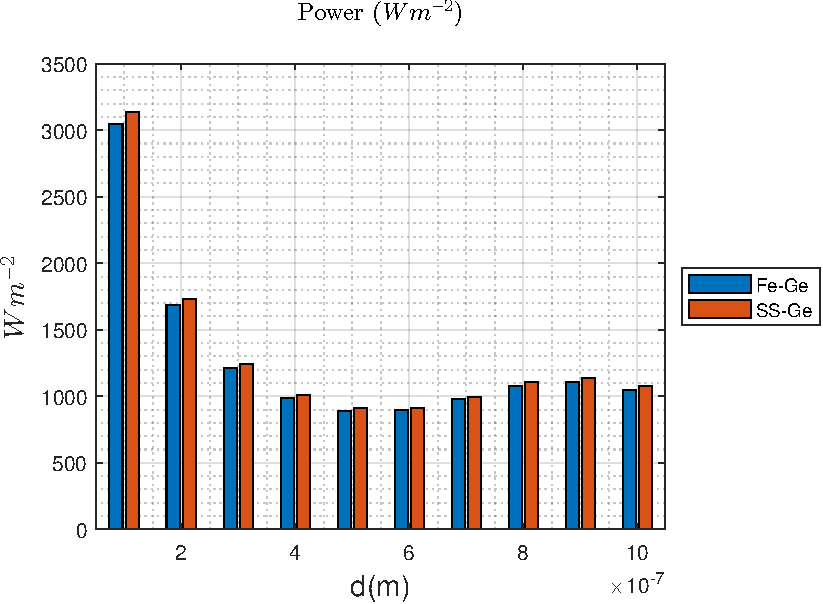
\includegraphics[width=0.65\textwidth]{figuras/rad_mat/FevsSs.pdf}
	\caption{Potencias por radiación integradas en el rango espectral de energía mayor a 0.7eV para un emisor de $Fe$ y un emisor de $SS$ con receptor de $Ge$ frente a las diferentes distancias de separación de las placas.}
	\label{fig:FevsSs}
\end{figure}
Se obtienen valores similares para todo el rango de distancias de separación estudiadas (figura \ref{fig:FevsSs}), de 100nm a 1000nm. Por lo tanto, se utiliza para las simulaciones de radiación de campo cercano el emisor de $SS$ con $n$ y $k$ extrapolados linealmente.\\\\
Se procede a simular la radiación por campo cercano para solo un emisor de $SS$ (figura \ref{fig:SsGe}), obteniéndose la potencia radiada espectral de la figura \ref{fig:rad_SiGe}. Se puede observar como esta potencia es menor que para el emisor de $Si$ (figura \ref{fig:rad_SiGe}) y también las potencias integradas en el rango espectral de energía superior a 0.7eV del emisor $SS$ (figura \ref{fig:p_Eg_SsGe}) son menores que para las del emisor de $Si$ (figura \ref{fig:p_Eg_SiGe}) para todas las distancias de separación.
\begin{figure}[H]
	\centering
	\begin{subfigure}[b]{0.49\textwidth}
	\centering
		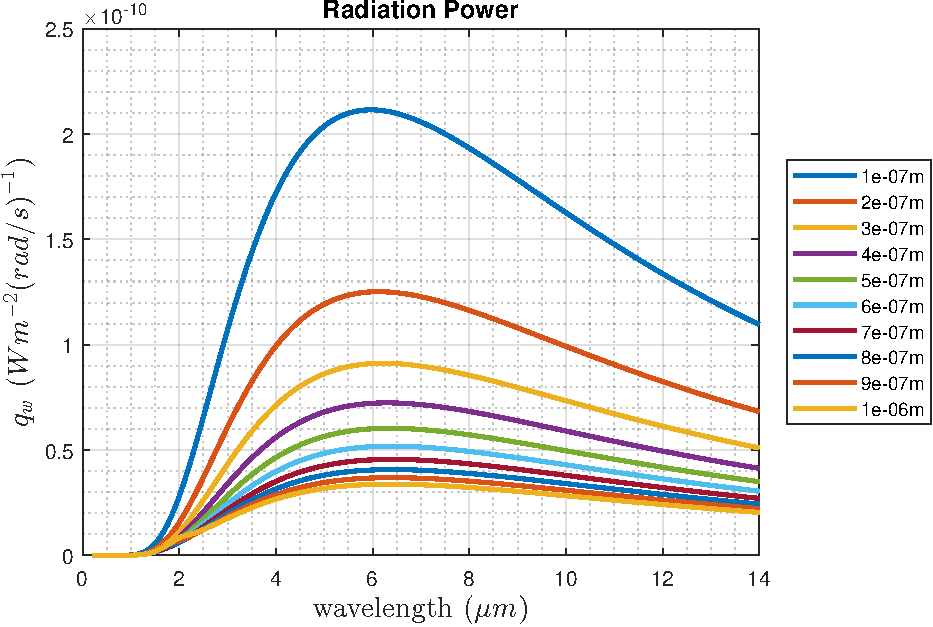
\includegraphics[width=1.00\textwidth]{figuras/Resultados/radiacion/SsGe.pdf}
	\caption{ }
	\label{fig:SsGe}
\end{subfigure}
\begin{subfigure}[b]{0.49\textwidth}
	\centering
		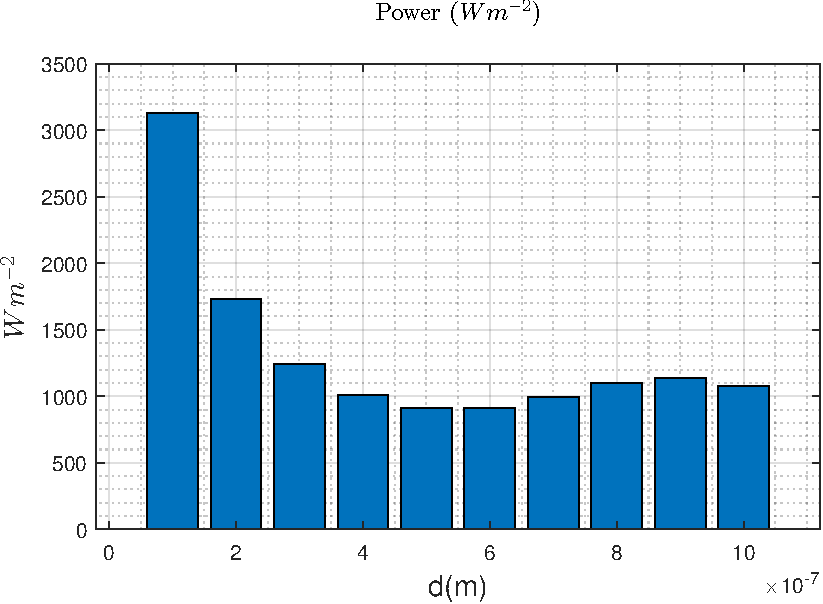
\includegraphics[width=1.00\textwidth]{figuras/Resultados/radiacion/p_Eg_SsGe.pdf}
	\caption{ }
	\label{fig:p_Eg_SsGe}
\end{subfigure}
\caption{(\subref{fig:SsGe}) Potencia radiada espectral ($q_w$) por campo cercano para un emisor de $SS$ y una célula de $Ge$. (\subref{fig:p_Eg_SsGe}) Potencia radiada para un rango de longitudes de onda cuya energía es mayor a los 0.7eV ($\sim 1.8 \ \mu m$).}
	\label{fig:rad_SsGe}
\end{figure}
Las potencias integradas no son todas mayores de 1000 $Wm^{-2}$ para las distancias de separación de 500nm, 600nm y 700nm, pero en promedio se pueden considerar que las potencias se encuentran en el rango de los miles de $Wm^{-2}$ desde los 300nm a los 1000nm, creciendo en mayor proporción a partir de los 200nm hasta los 100nm.
%%%   DENSIDAD DE NANO-ESPACIADORES
\subsection{Densidad de nano-espaciadores}
Se realizan los cálculos de las densidades de nano-espaciadores para las relaciones de las potencias de radiación respecto a las de conducción. Para el caso de la nTPV con $R_c$se gráfica solo para potencias de radiación 3 veces superior a las potencias de conducción. Para el caso con $R_c$ se gráfica para potencias de readiación de un orden de magnitud superior a las de conducción.
\begin{figure}[H]
	\centering
	\begin{subfigure}[b]{0.49\textwidth}
		\centering
			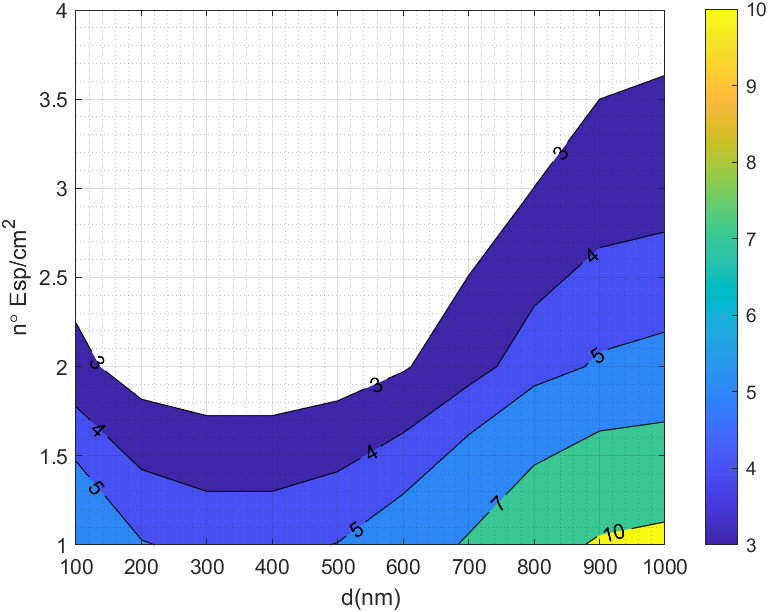
\includegraphics[width=1.00\textwidth]{figuras/Resultados/RelacionCondRad/SS.png}
		\caption{ }
		\label{fig:rel_SsSiO2Ge}
	\end{subfigure}
	\hfill
	\begin{subfigure}[b]{0.49\textwidth}
		\centering
			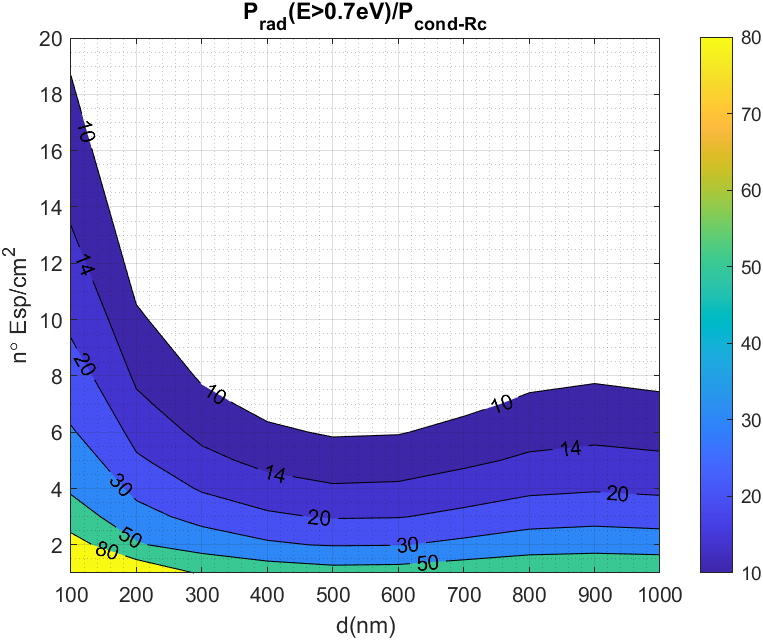
\includegraphics[width=1.00\textwidth]{figuras/Resultados/RelacionCondRad/SS_Rc_empirico.png}
		\caption{ }
		\label{fig:rel_SsSiO2Ge_Rc_emp}
	\end{subfigure}
	\caption{\small Relación entre la potencia radiada para energías mayores e igual a 0.7 eV y la potencia transmitida por conducción para distintas densidades de nano-espaciadores (eje y) y distintas alturas de los mismos (eje x), con (\subref{fig:rel_SsSiO2Ge_Rc_emp}) y sin (\subref{fig:rel_SsSiO2Ge}) $R_c$ térmica para una célula de 1 $cm^2$ y emisor de $SS$. La barra de colores lateral representa los colores asociados a cada uno de los valores de las relaciones de potencias, con los contornos de las relaciones más significativas representadas en las gráficas.
%	Densidades de nano-espaciadores para todas las relaciones de las potencias de radiación respecto a las conducción para un emisor de $SS$ frente a las altura de los nano-espaciadores para un emisor y una célula de 1 $cm^2$ sin $R_c$ (\subref{fig:rel_SsSiO2Ge}) y con $R_c$ empírica (\subref{fig:rel_SsSiO2Ge_Rc_emp}). El espectro de colores para cada relación entre las potencias de cada gráfica está indicado en las barra de colores lateral en el rango de valores que se encuentran en los extremos de cada barra.
	}
	\label{fig:rels_SsSiO2Ge_PnvsRc}
\end{figure}
Las densidades de nano-espaciadores obtenidas son menores que para la nTPV de $Si-SiO_2-Ge$ para todas las relaciones de potencias, siendo para el caso sin $R_c$ entre 1 a 2 nano-espaciadores menos por $cm^2$. Para las densidades de las nTPVs con $R_c$ para una altura de nano-espaciadores de 100nm la densidad disminuye de unos $\sim$30 $n^{\circ} esp/cm^2$ (figura \ref{fig:rel_SiSiO2Ge_Rc}) para la nTPV con emisor de $Si$ a unos $\sim$19 $n^{\circ} esp/cm^2$ (figura \ref{fig:rel_SsSiO2Ge_Rc_emp}) para la nTPV con emisor de $SS$ porque la potencia radiada es menor para el emisor de $SS$ que para el emisor de $Si$.
\begin{figure}[H]
	\centering
	\begin{subfigure}[b]{0.49\textwidth}
		\centering
			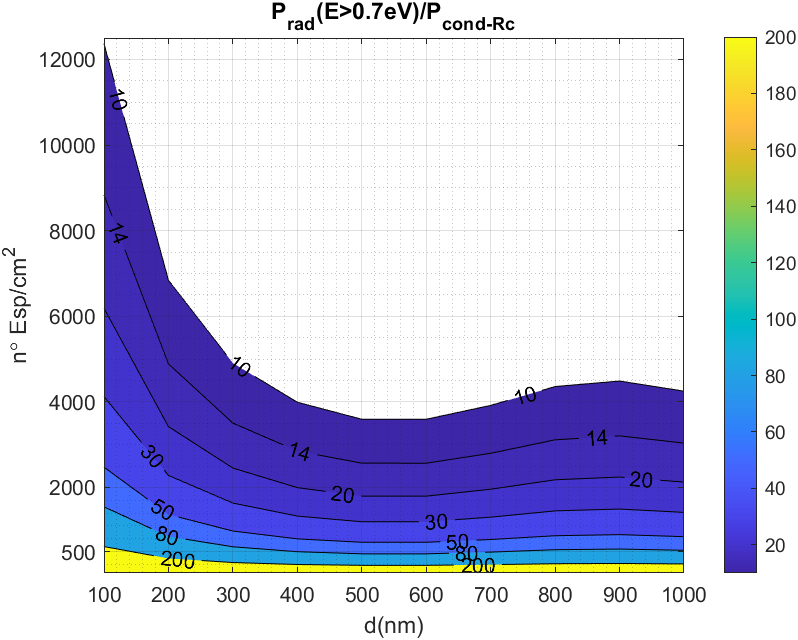
\includegraphics[width=1.00\textwidth]{figuras/Resultados/RelacionCondRad/SS_Rc_Intermedio.png}
		\caption{ }
		\label{fig:rel_SsSiO2Ge_Rc_inter}
	\end{subfigure}
	\hfill	
	\begin{subfigure}[b]{0.49\textwidth}
		\centering
			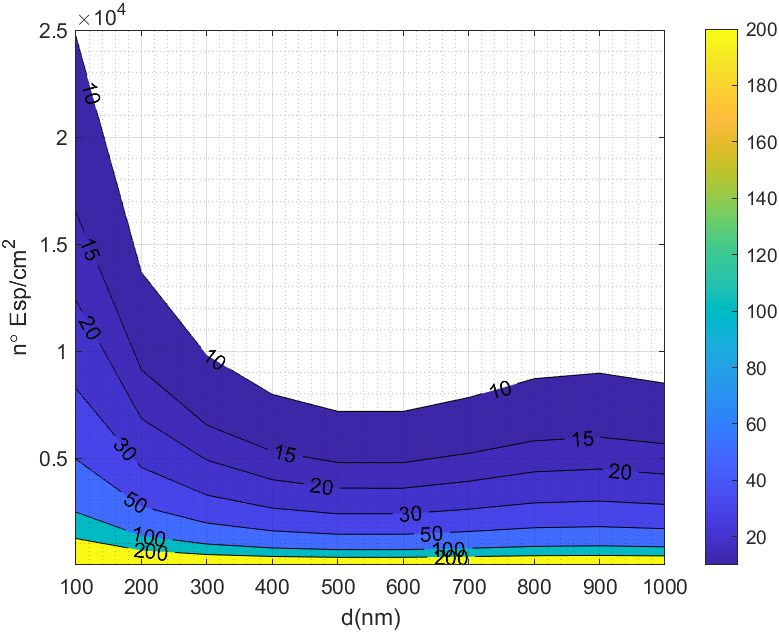
\includegraphics[width=1.00\textwidth]{figuras/Resultados/RelacionCondRad/SS_Rc.png}
		\caption{ }
		\label{fig:rel_SsSiO2Ge_Rc_max}
	\end{subfigure}
	\caption{\small Relación entre la potencia radiada para energías mayores e igual a 0.7 eV y la potencia transmitida por conducción para distintas densidades de nano-espaciadores (eje y) y distintas alturas de los mismos (eje x), con $R_c$ calculada intermedia (\subref{fig:rel_SsSiO2Ge_Rc_inter}) y con $R_c$ calculada máxima (\subref{fig:rel_SsSiO2Ge_Rc_max}) $R_c$ térmica para una célula de 1 $cm^2$ y un emisor de $SS$. La barra de colores lateral representa los colores asociados a cada uno de los valores de las relaciones de potencias, con los contornos de las relaciones más significativas representadas en las gráficas.
%Densidades de nano-espaciadores para todas las relaciones de las potencias de radiación respecto a las conducción para un emisor de $SS$ frente a las altura de los nano-espaciadores para un emisor y una célula de 1 $cm^2$ con $R_c$ calculada intermedia (\subref{fig:rel_SsSiO2Ge_Rc_inter}) y con $R_c$ calculada máxima (\subref{fig:rel_SsSiO2Ge_Rc_max}). El espectro de colores para cada relación entre las potencias de cada gráfica está indicado en las barra de colores lateral en el rango de valores que se encuentran en los extremos de cada barra.
}
	\label{fig:rels_SsSiO2Ge_Prc1vsPrc2}
\end{figure}
Para los casos con $R_c$ calculadas, las densidades de nano-espaciadores para una relación mínima de potencias de un orden de magnitud son del orden de $10^4 \ n^{\circ}esp/cm^2$ y disminuyendo al orden de los miles de $n^{\circ}esp/cm^2$ para relaciones de potencias de dos ordenes de magnitud. Para las relaciones de las potencias de dos ordenes de magnitud las densidades de nano-espaciadores a una altura de nano-espaciadores de 100nm son $\sim$ 2500 $n^{\circ} esp/cm^2$ para la nTPV con $R_c$ intermedia y $\sim$ 1000 $n^{\circ} esp/cm^2$ para la nTPV con $R_c$ máxima (figuras \ref{fig:rels_SsSiO2Ge_Prc1vsPrc2} \subref{fig:rel_SsSiO2Ge_Rc_inter} y \subref{fig:rel_SsSiO2Ge_Rc_max}).\\\\
Se observa que la relación entre las densidades de nano-espaciadores para ambos casos de $R_c$ calculada es aproximadamente igual a la relación entre ambas resistencias de contacto porque son constantes y solo afectan a la conducción en las simulaciones. El conocer estas relaciones es de utilidad para poder determinar en una primera instancia que valor de resistencia de contacto sería necesario como mínimo para tener la relación de potencias deseada con una cierta cantidad de nano-espaciadores de cierta altura.\\\\
También es importante tener en cuenta la variación de la densidad de nano-espaciadores o de la potencia de radiación entre su valor máximo y mínimo para una relación de potencias de un orden de magnitud porque las superficies tanto del emisor como de la célula presentan curvaturas que provocan un aumento o disminución de las distancias de separación entre ambos componentes, por ende, un aumento o disminución de las potencias de radiación útiles para su conversión en electricidad.\\\\
Para estudiar dicha variación, se calcula la reducción máxima de la densidad de nano-espaciadores para una relación de potencias de un orden de magnitud, suponiendo que todos los nano-espaciadores son de 100 nm de altura. Para el mejor caso se considera que la distancia de separación entre el emisor y la célula es igual a la altura de los nano-espaciadores, 100 nm, y para el peor caso es de 600 nm, por presentar la mayor y menor potencia de radiación, respectivamente.
Se obtiene que para todos los casos con $R_c$, la reducción de las densidades entre el mejor y peor caso supuestos es de un 70.95\%. Las nTPV con $R_c$ calculadas no se ven significativamente afectas por la reducción de la densidad de nano-espaciadores, a diferencia de la $R_c$ empírica, porque aún así la densidad es lo suficientemente alta para poder mantener una separación más estable entre le emisor y la célula, y mantener una relación de potencias más estable.\\\\
Por último, se recopilan los resultados obtenidos de las simulaciones en la tabla \ref{tab:SsSiO2Ge} para tener una mejor idea de los valores numéricos y de la magnitud de los resultados.
\begin{table}[H]
	\centering
	\caption{Tabla de recopilación de los resultados de las simulaciones de transmisión de calor por conducción y radiación de campo cercano para una nTPV de emisor de $SS$.}
		\begin{tabular}{|c||c|c|c|c||c|}
		\hline
		\multirow{2}{*}{ }& \multicolumn{5}{c|}{\textbf{\large Potencias según transmisión del calor}}\\ \cline{2-6}
& \multicolumn{4}{c||}{Conducción (W/nº esp.)}& Radiación $(W/m^2)$\\ \hline
Dist. (nm)&$P_{Normal}$&$P_{R_c-Cal.Max}$&$P_{R_c-Cal.Inter}$&$P_{R_c-Empirico}$&$P_{Eg>0.7eV}$\\ \hline \hline
100&4,80E-02&1,26815E-06&2,53438E-06&1,68E-03&3,13E+03\\ \hline 
200&3,42E-02&1,26813E-06&2,53431E-06&1,65E-03&1,73E+03\\ \hline 
300&2,64E-02&1,26811E-06&2,53424E-06&1,62E-03&1,24E+03\\ \hline 
400&2,15E-02&1,26809E-06&2,53417E-06&1,60E-03&1,01E+03\\ \hline 
500&1,81E-02&1,26808E-06&2,53410E-06&1,57E-03&9,11E+02\\ \hline 
600&1,56E-02&1,26806E-06&2,53403E-06&1,54E-03&9,10E+02\\ \hline 
700&1,37E-02&1,26804E-06&2,53396E-06&1,52E-03&9,93E+02\\ \hline 
800&1,22E-02&1,26802E-06&2,53388E-06&1,50E-03&1,10E+03\\ \hline 
900&1,11E-02&1,26800E-06&2,53381E-06&1,48E-03&1,14E+03\\ \hline 
1000&1,01E-02&1,26799E-06&2,53374E-06&1,45E-03&1,08E+03\\ \hline 
		\end{tabular}
	\label{tab:SsSiO2Ge}
\end{table}
\vfill \newpage
%%%%%%%%%%%%%%%%%%%%%%%%%%%%%%%%%%%
%%%%%%%%%%%    SiC-SiO2-Ge
\section{Resultados de las simulaciones para una nTPV de SiC-SiO2-Ge}\label{sec:res_SiCSiO2Ge}
Se procede a estudiar el caso de una nTPV con un emisor de Carburo de Silicio ($SiC$) por ser una material con mayor conductividad térmica que el $Si$ y el $SS$ a 800\textdegree C, que rondan unos 60 $W/(m^2 K)$ para el emisor de $SiC$, 26 $W/(m^2 K)$ para el $Si$ y 30 $W/(m^2 K)$ para el $SS$. Además el $SiC$ tiene un punto de fusión mayor que el $Si$ y el $SS$, siendo una característica del material de gran utilidad para su uso en baterías para almacenar la energía en forma de calor.\\\\
Otra razón de estudiar la nTPV con emisor de $SiC$ es por su utilización en \cite{doi:Near_field_ThinFilm} en una capa fina depositada sobre el emisor de una nTPV para aumentar el flujo de calor por radiación de campo cercano simulado entre el emisor y el receptor de $SiC$ grueso.
%%%%%    CFD
\subsection{Simulaciones de CFD}
\graphicspath{ {./figuras/Resultados/conduccion/pdf/} }
\begin{figure}[H]
	\centering
	\begin{subfigure}[b]{0.49\textwidth}
		\centering
			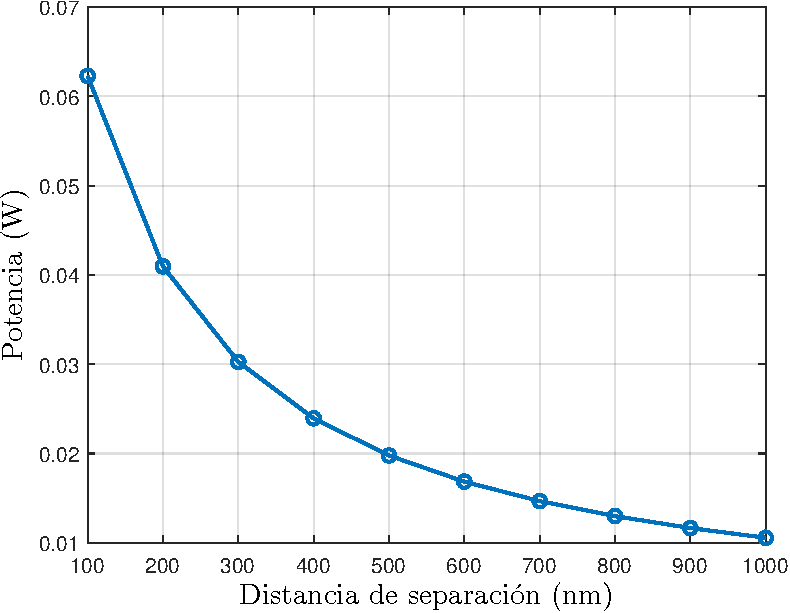
\includegraphics[width=1.00\textwidth]{Pn_SiCSiO2Ge.pdf}
		\caption{ }
		\label{fig:Prc_SiCSiO2Ge}
	\end{subfigure}
	\hfill
	\begin{subfigure}[b]{0.49\textwidth}
		\centering
			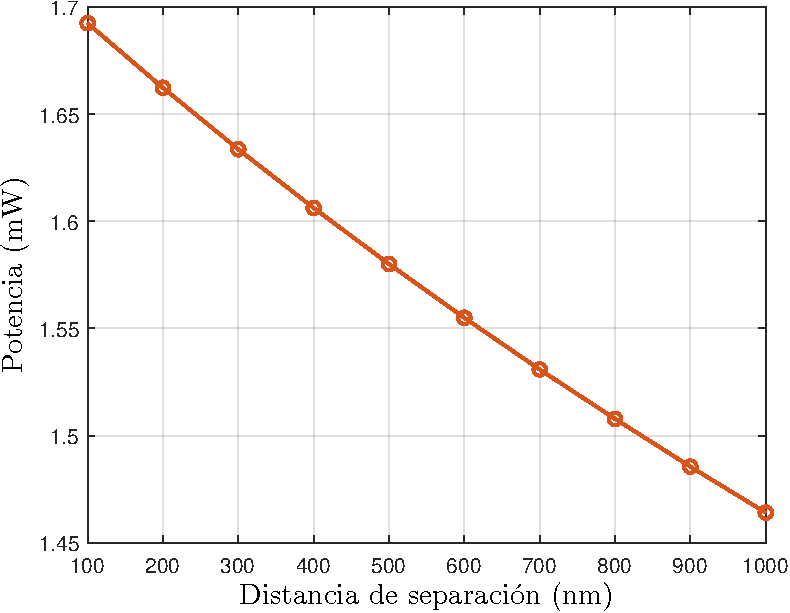
\includegraphics[width=1.00\textwidth]{Prc_SiCSiO2Ge.pdf}
		\caption{ }
		\label{fig:relPrc_SiCSiO2Ge}
	\end{subfigure}
	\caption{Potencias transmitidas por conducción para una nTPV $SiC-SiO_2-Ge$ sin $R_c$ (\subref{fig:Prc_SiCSiO2Ge}) y con $R_c$ empírica de $4\cdot 10^{-6} \ m^2 K/W$ (\subref{fig:relPrc_SiCSiO2Ge}) frente a las diferentes alturas de nano-espaciador.}
	\label{fig:PrcCond_SiCSiO2Ge}
\end{figure}
Se realizan las simulaciones de transmisión de calor por conducción, obteniéndose resultados similares a los casos anteriores porque la mayor cantidad de caída de temperatura se produce en el nano-espaciador por tener una baja conductividad térmica respecto al emisor y la célula. Algo que si se nota es que la potencia máxima es un 15.75\% mayor que para el emisor de $Si$, pero la reducción de las potencias con $R_c$ respecto a sin $R_c$ es menor, no superando el 86.14\% a los 1000nm. Siendo esta mayor que para el caso de la nTPV de emisor de $Si$, con una reducción de 85.69\% a los 1000 nm.\\\\
\subsection{Radiación de campo cercano}
Se realizan las simulaciones de transmisión de calor por radiación de campo cercano para el emisor de $SiC$, obteniéndose una potencia radiada espectral similar al del emisor de $Si$ para longitudes de onda menores a 2$\mu m$ (figura \ref{fig:rad_SiCGe}) y también tiene valores similares de la potencia radiada integrada en el rango espectral de energía mayor a 0.7eV frente a las distancias de separación respecto al emisor de $Si$ (figura \ref{fig:Prad_SiCGe}).
%%%           GRAFICAS
\graphicspath{ {./figuras/Resultados/radiacion} }
\begin{figure}[H]
	\centering
	\begin{subfigure}[b]{0.49\textwidth}
		\centering
		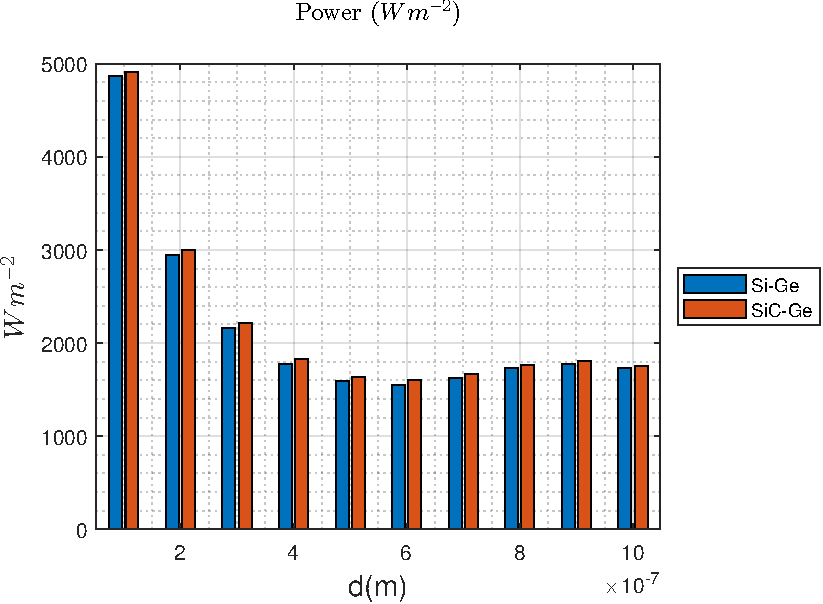
\includegraphics[width=1.00\textwidth]{SiCvsSi.pdf}
		\caption{ }
		\label{fig:Prad_SiCGe}
	\end{subfigure}
	\hfill
	\begin{subfigure}[b]{0.49\textwidth}
		\centering
		\includegraphics[width=1.00\textwidth]{SiCvsSi_rad.pdf}
		\caption{ }
		\label{fig:rad_SiCGe}
	\end{subfigure}
	\caption{(\subref{fig:Prad_SiCGe}) Potencias integradas en el rango espectral de energía mayor a 0.7eV para un emisor de $SiC$ y un emisor de $Si$ frente a las distancias de separación entre emisor y receptor. (\subref{fig:rad_SiCGe}) Potencia radiada espectral ($q_w$) para un emisor de $Si$ y $SiC$ con un receptor de $Ge$ para una distancia de separación de 100nm frente longitudes de onda.}
	\label{fig:rads_SiCGe}
\end{figure}
Aunque la potencia radiada espectral difiere al aumentar la longitud de onda ($\lambda$), no supone una gran diferencia entre ambos emisores porque en el rango energético de interés ($E>0.7eV$) las curvas son bastante similares, provocando que las potencias integradas en dicho rango energético sean similares también. Este rango se encuentra en la parte inferior izquierda de la figura \ref{fig:SiCSiC}, que va desde el origen hasta aproximadamente 1.8 $\mu m$.
\begin{figure}[H]
	\centering
		\includegraphics[width=0.65\textwidth]{figuras/Resultados/radiacion/SiCSiC.pdf}
	\caption{Potencias radiadas espectrales ($q_w$) frente a las longitudes de onda para un sistema de $SiC-SiC$ frente a diferentes distancias de separación entre placas.}
	\label{fig:SiCSiC}
\end{figure}
También se simula un sistema con receptor de $SiC$ y emisor de $SiC$ para observar los efectos de la \gls{wres} sobre las potencias de radiación frente a las longitudes de onda. Se observa en la figura \ref{fig:SiCSiC} que la \gls{wres} es aproximadamente $1.57\cdot 10^{14} \ rad/s$ ($\lambda = 12\mu m$) porque existe un pico de potencia espectral máxima que disminuye al aumentar la distancia de separación entre emisor y receptor, pudiéndose aprovechar dicha potencia para la conversión en electricidad si mediante una combinación de materiales se consigue que la frecuencia se encuentre dentro del rango espectral útil.
%%%    DENSIDAD
\subsection{Densidad de nano-espaciadores}
Se procede a calcular las densidades de nano-espaciadores por centímetro cuadrado para la nTPV con emisor de $SiC$ para los casos de sin $R_c$ y con $R_c$ de $4\cdot 10^{-6} \ m^2 K/W$ \cite{nf_TPV_Pillars_SiO2}. Obteniéndose unos resultados muy parecidos a los de la nTPV de emisor de $Si$ porque los resultados obtenidos de las simulaciones también son bastante cercanos.
\graphicspath{ {./figuras/Resultados/RelacionCondRad} }
\begin{figure}[H]
	\centering
	%% Si-SiO2-Si Eg
	\begin{subfigure}[b]{0.49\textwidth}
		\centering
		\includegraphics[width=1.00\textwidth]{SiC_Ge.png}
		\caption{ }
		\label{fig:rel_SiCSiO2Ge}
	\end{subfigure}
	\hfill
	\begin{subfigure}[b]{0.49\textwidth}
		\centering
		\includegraphics[width=1.00\textwidth]{SiC_Rc.png}
		\caption{ }
		\label{fig:rel_SiCSiO2Ge_Rc}
	\end{subfigure}
	\caption{\small
	Relación entre la potencia radiada para energías mayores e igual a 0.7 eV y la potencia transmitida por conducción para distintas densidades de nano-espaciadores (eje y) y distintas alturas de los mismos (eje x), con (\subref{fig:rel_SiCSiO2Ge_Rc}) y sin (\subref{fig:rel_SiCSiO2Ge}) $R_c$ térmica para una célula de 1 $cm^2$ y emisor de $SiC$. La barra de colores lateral representa todas las relaciones entre ambas potencias en el rango de los valores extremos que se muestran en la misma.
	%Densidades de nano-espaciadores ($n^{\circ}esp/cm^2$) frente a las alturas de los nano-espaciadores para todas las relaciones de la potencia de radiación en el rango espectral de energías mayores e igual a 0.7 eV respecto a las potencias de conducción (dependientes en la densidad de nano-espaciadores) mayores a 3 para el caso sin $R_c$ (\subref{fig:rel_SiCSiO2Ge}) y mayores a 10 para el caso con $R_c$ (\subref{fig:rel_SiCSiO2Ge_Rc}). Donde las barras de colores laterales de cada gráfica representan los colores asociados a cada uno de los valores de las relaciones de las potencias, con los contornos de las relaciones más significativas representadas en las gráficas.
	}
	\label{fig:relation_SiCSiO2Ge}
\end{figure}
La principal diferencia es en las densidades de nano-espaciadores para el caso de la nTPV sin $R_c$ (figura \ref{fig:rel_SiCSiO2Ge}), siendo esta menor que la del emisor de $Si$ para todo el rango de alturas de los nano-espaciadores porque la conductividad térmica del $SiC$ a 800\textdegree C es mayor que para el $Si$ por lo tanto la resistencia térmica del sistema disminuye, teniendo así unas menores densidades. Para el caso de la nTPV con $R_c$, las diferencias no son tan notables como en el caso sin $R_c$ porque la componente con mayor relevancia es la resistencia de contacto.\\\\
Por último, se recopilan los resultados obtenidos de las simulaciones de transferencia de calor por conducción y radiación de campo cercano en la tabla \ref{tab:SiCSiO2Ge}, los resultados se muestran en notación científica para simplificar el análisis de los mismos.
\begin{table}[h]
	\centering
	\caption{Tabla de recopilación de los resultados de las simulaciones de transmisión de calor por conducción y radiación de campo cercano para una nTPV de emisor de $SiC$.}
		\begin{tabular}{|c||c|c||c|c|}
		\hline
\multirow{2}{*}{ }& \multicolumn{4}{c|}{\textbf{\large Potencias según transmisión del calor}}\\ \cline{2-5}
& \multicolumn{2}{c||}{Conducción (W/nº esp.)}& \multicolumn{2}{c|}{Radiación $(W/m^2)$}\\ \hline
Dist. (nm)&$P_{Normal}$&$P_{R_c-Empirico}$&$P_{Eg>0.7eV}$&$P_{full}$\\ \hline \hline
100&6,23E-02&1,69E-03&4,90E+03&1,50E+05\\ \hline 
200&4,09E-02&1,66E-03&3,00E+03&1,01E+05\\ \hline 
300&3,03E-02&1,63E-03&2,21E+03&7,80E+04\\ \hline 
400&2,39E-02&1,61E-03&1,82E+03&6,43E+04\\ \hline 
500&1,98E-02&1,58E-03&1,64E+03&5,52E+04\\ \hline 
600&1,68E-02&1,55E-03&1,60E+03&4,87E+04\\ \hline 
700&1,47E-02&1,53E-03&1,67E+03&4,40E+04\\ \hline 
800&1,30E-02&1,51E-03&1,76E+03&4,06E+04\\ \hline 
900&1,17E-02&1,49E-03&1,81E+03&3,80E+04\\ \hline 
1000&1,06E-02&1,46E-03&1,75E+03&3,61E+04\\ \hline 
		\end{tabular}
	\label{tab:SiCSiO2Ge}
\end{table}

\vfill \newpage
%%%%%%%%%%%%%%%%%%%%%%%%%%%%%%%%%%%%%%%%%%%%
%%%     NUMERO DE NANO-ESPACIADORES
%%%%%%%%%%%%%%%%%%%%%%%%%%%%%%%%%%%%%%%%%%%%
\section{Densidad de nano-espaciadores para soportar la carga}\label{sec:densidad_carga}
Dado que los nano-espaciadores tendrán que soportar el peso del emisor o la célula se estudia la cantidad mínima de nano-espaciadores necesarios en un centímetro cuadrados para soportar la carga. También se estudia la densidad de nano-espaciadores para el caso de que se aplique una presión de una atmósfera a una de las caras para asegurar que las distancias de separación sean lo más uniformes posibles.\\\\
La resistencia a compresión del $SiO_2$ es de unos $1.16 \ GPa$\footnote{El valor se ha obtenido de la base de datos de \hyperref[sec:grantaEduPack]{Granta EduPack 2021 R2} para el $SiO_2$ de nombre \textbf{Silica (quartz fused)}, que presenta una pureza del 99.9\%} y la densidad mayor entre los materiales de emisor y células es el acero inoxidable 304, con una densidad aproximada de $8 \ g/cm^3$ o $8\cdot 10^3 kg/m^3$. Para un emisor $SS$ de área $1 \ cm^2$ y espesor de $0.5 \ cm$ la masa total es de unos 4 $gr$ o un peso de unos $\sim 0.04 \ N$, obteniéndose una densidad mínima de nano-espaciadores para solo soportar la carga del emisor de $4 \ n^{\circ}esp/cm^2$, un valor bastante pequeño para disminuir las curvaturas por flexión o imperfecciones del acabado de la superficie del emisor, pero teniendo una mayor relación entre las potencias de radiación respecto a las de conducción, es decir, mayor transferencia de potencia útil respecto a las pérdidas por conducción, disminuyendo así el aumento indeseado de la temperatura de la célula.\\\\
Al aplicarse una presión de una atmósfera sobre la superficie superior del emisor de la nTPV, la fuerza que soportan los nano-espaciadores aumenta hasta los $10.17 \ N$ generando que se necesiten una densidad mínima de nano-espaciadores de $975 \ n^{\circ}esp/cm^2$ para poder soportar la carga. Está densidad mínima es bastante alta respecto a las obtenidas en todos los casos de nTPVs de célula de germanio estudiados con resistencia de contacto empírica de $4\cdot 10^{-6} \ m^2 K/W$, pero no es tan elevada para el caso de la nTPV $SS-SiO_2-Ge$ con las $R_c$ calculadas para una relación de potencias mayor de un orden de magnitud (figuras \ref{fig:rels_SsSiO2Ge_Prc1vsPrc2} \subref{fig:rel_SsSiO2Ge_Rc_inter} y \subref{fig:rel_SsSiO2Ge_Rc_max}) porque sus valores de $R_c$ son mayores que la $R_c$ empírica y por ende, disminuyen las pérdidas que provoca un aumento de las densidades.
\vfill \newpage
%%%%%%%%%%%%%%%%%%%%%%%%%%%%%%%%%%%%%%%%%%%%%%%%%%%%%%%%%%%
%%    COMPARACION MATERIAL NANO-ESPACIADORES  Ctrl+Q to comment and Ctrl+W to uncomment
%%%%%%%%%%%%%%%%%%%%%%%%%%%%%%%%%%%%%%%%%%%%%%%%%%%%%%%%%%%%%
\section{Resultados de las simulaciones para unas nTPVs de nano-espaciadores de Si}\label{sec:res_XxSiGe}
\graphicspath{ {./figuras/Resultados/DiffMatEsp} }
Como último caso de simulación se simula la transmisión de calor en CFD por conducción para una nTPV de nano-espaciador de $Si$ y un emisor de $SiC$ con resistencias de contacto empíricas de $4\cdot 10^{-6} \ m^2 K/W$, por si durante el proceso de deposición del nano-espaciador no se llegara a conseguir depositar $SiO_2$ sino un material con características semejantes a las del $Si$, esto ya ha sucedido en unos ensayos para la fabricación de los nano-espaciadores en la IES. 
%Esto sucede porque durante unas pruebas de fabricación del $SiO_2$ en la IES, no siempre se consiguía $SiO_2$ de buena calidad y que en el peor de los casos el $SiO_2$ fabricado podría tener unas características más similares al $Si$ que al $SiO_2$ ideal.
% comparar el efecto de cambiar el material del nano-espaciador
\begin{table}[H]
	\centering
	\caption{Tabla de recopilación de los resultados de las simulaciones de transferencia de calor por conducción para las nTPVs con nano-espaciador de Si y emisores de $Si$, $SS$ y $SiC$ respecto a cada altura del nano-espaciador.}
		\begin{tabular}{|c||c|c|c|}
		\hline
		 \multicolumn{4}{|c|}{\textbf{Potencias de Conducción ($mW$)}}\\	\hline
		Dist. (nm)&$P_{R_c-Si}$&$P_{R_c-SS}$&$P_{R_cSiC}$\\ \hline \hline 
		100&$1.7136$&$1.7113$&$1.7261$\\ \hline 
		200&$1.7135$&$1.7112$&$1.7260$\\ \hline 
		300&$1.7134$&$1.7110$&$1.7258$\\ \hline 
		400&$1.7132$&$1.7109$&$1.7257$\\ \hline 
		500&$1.7130$&$1.7107$&$1.7255$\\ \hline 
		600&$1.7128$&$1.7105$&$1.7252$\\ \hline 
		700&$1.7126$&$1.7103$&$1.7250$\\ \hline 
		800&$1.7125$&$1.7102$&$1.7249$\\ \hline 
		900&$1.7122$&$1.7099$&$1.7246$\\ \hline 
		1000&$1.7121$&$1.7098$&$1.7244$\\ \hline
		\end{tabular}
	\label{tab:nanoEspaciadorDeSi}
\end{table}
En primer lugar, de los resultados de las simulaciones de CFD, recopiladas en la tabla \ref{tab:nanoEspaciadorDeSi}, se observa como las pérdidas de conducción son mayores para los nano-espaciadores de $Si$ (figura \ref{fig:prc_xxSi}) que para los nano-espaciador de $SiO_2$ (figura \ref{fig:prc_xxSiO2}) porque la conductividad del $Si$ es mayor que la del $SiO_2$. Por lo tanto, la resistencia térmica del nano-espaciador es menos significativa y la resistencia de contacto tiene una mayor importancia.
\begin{figure} [H]%
	\centering
	\begin{subfigure}[b]{0.48\textwidth}%
			\includegraphics[width=\columnwidth]{Prc_XxSiGe}%
			\caption{}%
			\label{fig:prc_xxSi}%
	\end{subfigure}
	\hfill
	\begin{subfigure}[b]{0.48\textwidth}%
			\includegraphics[width=\columnwidth]{Prc_XxSiO2Ge}%
			\caption{}%
			\label{fig:prc_xxSiO2}%
	\end{subfigure}
	\caption{Potencias transmitidas por conducción de unas nTPVs con emisores de $Si$, $SS$ y $SiC$ frente a las alturas de un solo nano-espaciador en nanometros para un nano-espaciador de $Si$ (\subref{fig:prc_xxSi}) y para un nano-espaciador de $SiO_2$ (\subref{fig:prc_xxSiO2}).}%
	\label{fig:prc_xxXX}%
\end{figure}
En segundo lugar, se observa como las curvas de las potencias de conducción no varían tanto entre su valor máximo y valor mínimo, siendo para el caso de las nTPVs con nano-espaciadores de $Si$ el que presenta la menor variación de los dos, siendo esta menor de $0.002 \ mW$ (figura \ref{fig:prc_xxSi}), a diferencia de los nano-espaciadores de $SiO_2$ cuya variación es menor a los $0.25 \ mW$ (figura \ref{fig:prc_xxSiO2}). También se observa con mayor detalle como la diferencias de las resistencias térmicas de los materiales afecta al flujo de calor, aumentando con la disminución de la resistencia térmica o aumento de la conductividad térmica, cuyos valores se mencionan en la sección \ref{sec:res_SiCSiO2Ge}.\\\\
En tercer lugar, las potencias de conducción son muy similares para ambos materiales de nano-espaciador con la altura de 100 nm porque la resistencia térmica de los nano-espaciadores disminuye considerablemente con la disminución de la distancia, por ser proporcional a ella. Esto produce que la $R_c$ sea la principal resistencia térmica del sistema, por tal motivo, los valores de las potencias de conducción se asemejan a dicha altura del nano-espaciador.\\\\
Por último, se calculan las densidades de nano-espaciadores frente a las alturas de los nano-espaciadores para la nTPV de emisor de $SiC$ y nano-espaciadores de $Si$ (figura \ref{fig:prc_SiCSi}), y se compara con las densidades de la nTPV de emisor de $SiC$ pero nano-espaciadores de $SiO_2$ (figura \ref{fig:prc_SiCSiO2}). Se observa que existe una disminución de las densidades para cada relación de potencias y todas las alturas de los nano-espaciadores, siendo la más notable a los 1000 nm de altura y relación de potencias de un orden de magnitud, pasando la densidad de ser $12 \ n^{\circ}esp/cm^2$ (figura \ref{fig:prc_SiCSiO2}) a ser $10 \ n^{\circ}esp/cm^2$ (figura \ref{fig:prc_SiCSi}). Esta poca variación para dos materiales distintos de nano-esapciadores se dá porque para ambos casos la nTPV tiene una $R_c$ que es la resistencia térmica más significativa del sistema.
\begin{figure} [h]%
	\centering
	\begin{subfigure}[b]{0.48\textwidth}%
			\includegraphics[width=\columnwidth]{rel_SiC}%
			\caption{}%
			\label{fig:prc_SiCSi}%
	\end{subfigure}
	\hfill
	\begin{subfigure}[b]{0.48\textwidth}%
			\includegraphics[width=\columnwidth]{SiC_Rc}%
			\caption{}%
			\label{fig:prc_SiCSiO2}%
	\end{subfigure}
	\caption{\small
	Relación entre la potencia radiada para energías mayores e igual a 0.7 eV y la potencia transmitida por conducción con $R_c$ para distintas densidades de nano-espaciadores (eje y) y distintas alturas de los mismos (eje x), para nTPV de 1 $cm^2$ con nano-espaciadores de $Si$ (\subref{fig:prc_SiCSi}) y de $SiO_2$ (\subref{fig:prc_SiCSiO2}). 
	La barra de colores lateral representa los colores asociados a cada uno de los valores de las relaciones de potencias, con los contornos de las relaciones más significativas representadas en las gráficas.
	%Densidades de nano-espaciadores ($n^{\circ}esp/cm^2$) frente a las alturas de los nano-espaciadores para todas las relaciones de la potencia de radiación en el rango espectral de energías mayores e igual a 0.7 eV respecto a las potencias de conducción con $R_c$ (dependientes en la densidad de nano-espaciadores) mayores a 10 para nTPVs de nano-espaciadores de $Si$ (\subref{fig:prc_SiCSi}) y $SiO_2$(\subref{fig:prc_SiCSiO2}) . Donde las barras de colores laterales de cada gráfica representan los colores asociados a cada uno de los valores de las relaciones de las potencias, con los contornos de las relaciones más significativas representadas en las gráficas.
	}%
	\label{fig:prc_SiCXX}%
\end{figure}

%%\chapter{Gestión del proyecto}

En este capítulo se describe la gestión del proyecto: ciclo de vida, planificación, presupuesto, etc.

\section{Ciclo de vida}

Explicación de las fases del proyecto: definición, análisis, diseño, construcción, pruebas, implementación, validación, documentación. Ejemplo: diagrama de Pert.

\section{Planificación}

Se puede indicar mediante un diagram de Gantt.

\subsection{Planificación inicial}

\subsection{Planificación final}


\section{Presupuesto}

\subsection{Personal}

\subsection{Material}

\subsection{Resumen de costes}

\chapter{Conclusiones}

Se presentan a continuación las conclusiones...

\section{Conclusión}

Una vez finalizado el proyecto...

\section{Desarrollos futuros}

Un posible desarrollo...

\appendix

\chapter[Procedimientos simulaciones radiación]{Procedimientos seguidos para la realización de las simulaciones de radiación de campo cercano}\label{ch:procedimientosSimRad}

En este apéndice se detallan los pasos genéricos seguidos para la realización de las simulaciones de radiación de campo cercano y la obtención de los resultados de las potencias integradas en un respectivo rango espectral utilizando la aplicación \textbf{calculadora de campo cercano}, descrita en la sección \ref{sec:calc_campo_cercano}.

\section{Procedimientos genéricos}
Existen solo cuatro posibles casos de simulaciones de transmisión de calor por radiación de campo cercano utilizando la aplicación, estos casos son los siguientes:
\begin{itemize}
	\item Una distancia de separación y un par de materiales, uno para el emisor y otro para el receptor.
	\item Rango de distancias de separación y un par de materiales.
	\item Una distancia de separación y varias combinaciones de materiales.
	\item Rango de distancias de separación y varias combinaciones de materiales.
\end{itemize}
Los procedimientos para la realización de las simulaciones de transmisión de calor por radiación de campo cercano siguen el mismo orden de ejecución genérico. Estos procedimientos son:
\begin{itemize}
	\item Selección de la temperatura del emisor, que para este trabajo se mantiene a 1073K (800\textdegree C).
	\item Selección de las combinaciones de materiales a simular.
	\item Selección del rango de distancias a simular.
	\item Hacer clic sobre el botón \textbf{Calculate}.
\end{itemize}
%%%%%%%%%%%%%%%%%%%%%%%%%%%%%%%%%%%%%%%%%%%%%%%%%%%%%%%%%%5
%%%%%%%%%%%%%%%%%%%%%%%%%%%%%%%%%%%%%%%%%%%%%%%%%%%%%%%%%%
\section{Distancia fija y un par de materiales}
Se siguen los siguientes pasos:
\begin{enumerate}
	\item Seleccionar el material de la placa superior en \textbf{Superior plate} (figura \ref{unParMat}). 
	\item Seleccionar el material de la placa inferior en \textbf{Inferior plate}.
	\item Seleccionar la distancia (figura \ref{unaDistancia}). 
%%%%%
\begin{figure}[H]
\centering
\begin{subfigure}[b]{.48\textwidth}
	\centering
		\includegraphics{figuras/unaDistancia.PNG}
	\caption{ }
	\label{unaDistancia}
\end{subfigure} \hfill
\begin{subfigure}[b]{.48\textwidth}
	\centering
		\includegraphics{figuras/unParMat.PNG}
		\caption{ }
	\label{unParMat}
\end{subfigure}
\caption{Seleccionador de una distancia de separación en nanometros (\subref{unaDistancia}) y seleccionar de los materiales de emisor (Superior plate) y receptor (Inferior plate) (\subref{unParMat}) de la calculadora de campo cercano.}
\label{fig:sencillo}
\end{figure}	
	\item Hacer click sobre el botón \textbf{Calculate}.
	\item Esperar que el indicador de estado pase de \textit{Running...}, color rojo del indicador (figura \ref{fig:indicador_Running2}), a \textit{StdBy}, color verde del indicador (figura \ref{fig:indicador_StdBy2}), es decir, esperar que termine la simulación.
	\end{enumerate}
		%% figuras de estados
	\begin{figure}[H]
	\centering
	%% Figura 1
	\begin{subfigure}[b]{0.3\textwidth}
	\centering
	\includegraphics[width=\textwidth]{figuras/Procedimiento_Simulaciones/Radiacion/estado_changed}%
	\caption{Changed}%
	\label{fig:indicador_Changed2}%
	\end{subfigure}
	\hfill
	%% Figura 2
	\begin{subfigure}[b]{0.3\textwidth}
	\centering
	\includegraphics[width=\textwidth]{figuras/Procedimiento_Simulaciones/Radiacion/estado_running}%
	\caption{Running}%
	\label{fig:indicador_Running2}%
	\end{subfigure}
	\hfill
	%% Figura 3
	\begin{subfigure}[b]{0.3\textwidth}
	\centering
	\includegraphics[width=0.9\textwidth]{figuras/Procedimiento_Simulaciones/Radiacion/estado_stdby}%
	\caption{StdBy}%
	\label{fig:indicador_StdBy2}%
	\end{subfigure}
	\hfill
	\caption{Indicadores del estado actual del sistema. (\subref{fig:indicador_Changed2}) Indicador del estado \textbf{Changed} o estado de cambio, se activa cuando se produce algún cambio en los datos seleccionados para simular. (\subref{fig:indicador_Running2}) Indicador del estado \textbf{Running} o corriendo, se activa cuando estando en el estado \textbf{Changed} se hace clic al botón \textbf{Calculate} y corre la simulación. (\subref{fig:indicador_StdBy2}) Indicador del estado \textbf{StdBy}, se activa cuando termina la simulación, avisando que está a la espera de algún cambio.}
	\label{fig:indicadorLED2}
	\end{figure}
	%%%%%%%%%%%%%%%%%%%%%%%%%%%%%%%%%%%%%%%%%%%%%%%%%%%%%%%%%%%%%
%%%%%%%%%%%%%%%%%%%%%%%%%%%%%%%%%%%%%%%%%%%%%%%%%%%%%%%%%%%%%%%
\section{Rango de distancias y un par de materiales}
\begin{enumerate}
	\item Seleccionar el material de la placa superior en \textbf{Superior plate} (figura \ref{unParMat}).
	\item Seleccionar el material de la placa inferior en \textbf{Inferior plate}.
	\item Hacer click sobre el checkbox \textbf{Distance Range} (figura \ref{fig:check_distances2}).
	\item Hacer click sobre el botón \textbf{set} del \textbf{Distance Range}, que produce que aparezca la ventana de la figura \ref{fig:set_distances2}.
	\item Seleccionar el rango de distancias deseado o el checkbox \textbf{Full Range}, según lo que se desee. Para este trabajo se selecciona el checkbox \textbf{Full Range}.
	\item Hacer click en \textbf{Accept} de la nueva ventana.
	\item Hacer click sobre el botón \textbf{Calculate} y esperar a que termine de ejecutarse la simulación.
\end{enumerate}
	\begin{figure}[H]%
	\begin{subfigure}[b]{0.48\textwidth}
		\centering
			\includegraphics[width=0.6\textwidth]{figuras/Procedimiento_Simulaciones/Radiacion/check_distances2.png}
		\caption{Checkbox de distancias}
		\label{fig:check_distances2}
	\end{subfigure}
	\hfill
	\begin{subfigure}[b]{0.48\textwidth}
		\centering
			\includegraphics[width=0.6\textwidth]{figuras/Procedimiento_Simulaciones/Radiacion/set_distances_fullrange.png}
		\caption{Set de distancias}
		\label{fig:set_distances2}
	\end{subfigure}
	\caption{(\subref{fig:check_distances2}) Casilla para la selección de la opción de simular un rango de distancias. (\subref{fig:set_distances2}) Ventana para la selección del rango de distancias a simular.}%
	\label{fig:checkboxes2}%
	\end{figure}
	%%%%%%%%%%%%%%%%%%%%%%%%%%%%%%%%%%%%%%%%%%%%%%%%%%%
	%%%%%%%%%%%%%%%%%%%%%%%%%%%%%%%%%%%%%%%%%%%%%%%%%%%
	\section{Distancia fija y varios materiales}
	\begin{enumerate}
			\item Hacer click sobre el checkbox \textbf{Materials Range} (figura \ref{fig:check_materials2}).
			\item Hacer click sobre el botón \textbf{set} del \textbf{Materials Range}, que produce que aparezca la ventana de la figura \ref{fig:set_materials2}.
			\item Seleccionar los materiales para la cara superior (UpFace) (figura \ref{fig:set_materials2}).
			\item Seleccionar los materiales para la cara inferior (DownFace).
			\item Hacer clic en \textbf{Accept} de la ventana emergente.
			\item Seleccionar la distancia (figura \ref{unaDistancia}). 
			\item Hacer click sobre el botón \textbf{Calculate} y esperar a que termine de ejecutarse la simulación.
	\end{enumerate}
	%%%%%%%%%%%%%%%%%
	\begin{figure}[H]%
	\begin{subfigure}[b]{0.48\textwidth}
		\centering
			\includegraphics[width=0.6\textwidth]{figuras/Procedimiento_Simulaciones/Radiacion/set_materilas2.png}
		\caption{Set de materiales}
		\label{fig:set_materials2}
	\end{subfigure}\hfill
		\begin{subfigure}[b]{0.48\textwidth}
		\centering
			\includegraphics[width=0.6\textwidth]{figuras/Procedimiento_Simulaciones/Radiacion/check_materials2.png}
		\caption{Checkbox de materiales}
		\label{fig:check_materials2}
	\end{subfigure}
	\caption{(\subref{fig:set_materials2}) Ventana para la selección de las combinaciones de materiales a simula, siendo \textbf{UpFace} el emisor y \textbf{DownFace} la célula.	(\subref{fig:check_materials2}) Casilla para la selección de la opción de simular una combinación de materiales.}%
	\label{fig:sets2}%
	\end{figure}	
	%%%%%%%%%%%%%%%%%%%%%%%%%%%%%%%%%%%%%%%%%%%%%%%%%%%%
	%%%%%%%%%%%%%%%%%%%%%%%%%%%%%%%%%%%%%%%%%%%%%%%%%%%%
\section{Rango de materiales y varios materiales}
\begin{enumerate}
			\item Hacer click sobre el checkbox \textbf{Materials Range} (figura \ref{fig:check_materials2}).
			\item Hacer click sobre el checkbox \textbf{Distance Range} (figura \ref{fig:check_distances2}).
			%% MATERIALS
			\item Hacer click sobre el botón \textbf{set} del \textbf{Materials Range}, que produce que aparezca la ventana de la figura \ref{fig:set_materials2}.
			\item Seleccionar los materiales para la cara superior (UpFace) (figura \ref{fig:set_materials2}).
			\item Seleccionar los materiales para la cara inferior (DownFace).
			\item Hacer clic en \textbf{Accept} de la ventana emergente.
			%%%% DISTANCE
			\item Hacer click sobre el botón \textbf{set} del \textbf{Distance Range}, que produce que aparezca la ventana de la figura \ref{fig:set_distances2}.
			\item Seleccionar el rango de distancias deseado o el checkbox \textbf{Full Range}, según lo que se desee. Para este trabajo se selecciona el checkbox \textbf{Full Range}.
			\item Hacer click en \textbf{Accept} de la nueva ventana.
			\item Hacer click sobre el botón \textbf{Calculate} y esperar a que termine de ejecutarse la simulación.
\end{enumerate}

\backmatter
%Glosario, lista de símbolos, notas, etc.

%estilo de bibliografía: plana, alfa...
\bibliographystyle{plain}

%genera doble hoja en blanco
\cleardoublepage

%apartado de bibliografía
\addcontentsline{toc}{chapter}{Bibliografia}

%se incluye la bibliografía. Archivo de tipo .bib (bibtex)
\bibliography{bibliografia/bibliografia}


% Se incluye los anexos
%\appendix

\chapter{Anexo: Documentación de la librería Travis}

{\Large Se muestra a continuación la documentación del código de la librería Travis, realizada con un generador de documentación automático. En nuestro caso, el documentador elegido es Doxygen.}


%fin del documento
\end{document}